%definira klasu dokumenta 
\documentclass[12pt]{report} 

%prostor izmedu naredbi \documentclass i \begin{document} se zove uvod. U njemu se nalaze naredbe koje se odnose na cijeli dokument

%osnovni LaTex ne može riješiti sve probleme, pa se koriste različiti paketi koji olakšavaju izradu željenog dokumenta
\usepackage[croatian]{babel} 
\usepackage{amssymb}
\usepackage{amsmath}
\usepackage{txfonts}
\usepackage{mathdots}
\usepackage{titlesec}
\usepackage{array}
\usepackage{lastpage}
\usepackage{etoolbox}
\usepackage{tabularray-2021}
\usepackage{color, colortbl}
\usepackage{adjustbox}
\usepackage{geometry}
\usepackage[classicReIm]{kpfonts}
\usepackage{hyperref}
\usepackage{fancyhdr}

\usepackage{float}
\usepackage{setspace}
\restylefloat{table}


\patchcmd{\chapter}{\thispagestyle{plain}}{\thispagestyle{fancy}}{}{} %redefiniranje stila stranice u paketu fancyhdr

%oblik naslova poglavlja
\titleformat{\chapter}{\normalfont\huge\bfseries}{\thechapter.}{20pt}{\Huge}
\titlespacing{\chapter}{0pt}{0pt}{40pt}


\linespread{1.3} %razmak između redaka

\geometry{a4paper, left=1in, top=1in,}  %oblik stranice

\hypersetup{ colorlinks, citecolor=black, filecolor=black, linkcolor=black,	urlcolor=black }   %izgled poveznice


%prored smanjen između redaka u nabrajanjima i popisima
\newenvironment{packed_enum}{
	\begin{enumerate}
		\setlength{\itemsep}{0pt}
		\setlength{\parskip}{0pt}
		\setlength{\parsep}{0pt}
	}{\end{enumerate}}

\newenvironment{packed_item}{
	\begin{itemize}
		\setlength{\itemsep}{0pt}
		\setlength{\parskip}{0pt}
		\setlength{\parsep}{0pt}
	}{\end{itemize}}




%boja za privatni i udaljeni kljuc u tablicama
\definecolor{LightBlue}{rgb}{0.9,0.9,1}
\definecolor{LightGreen}{rgb}{0.9,1,0.9}

%Promjena teksta za dugačke tablice
\DefTblrTemplate{contfoot-text}{normal}{Nastavljeno na idućoj stranici}
\SetTblrTemplate{contfoot-text}{normal}
\DefTblrTemplate{conthead-text}{normal}{(Nastavljeno)}
\SetTblrTemplate{conthead-text}{normal}
\DefTblrTemplate{middlehead,lasthead}{normal}{Nastavljeno od prethodne stranice}
\SetTblrTemplate{middlehead,lasthead}{normal}

%podesavanje zaglavlja i podnožja

\pagestyle{fancy}
\lhead{Programsko inženjerstvo}
\rhead{Svjetski putnik}
\lfoot{DJUNGELSKOG}
\cfoot{stranica \thepage/\pageref{LastPage}}
\rfoot{\today}
\renewcommand{\headrulewidth}{0.2pt}
\renewcommand{\footrulewidth}{0.2pt}


\begin{document} 
	
	
	
	\begin{titlepage}
		\begin{center}
			\vspace*{\stretch{1.0}} %u kombinaciji s ostalim \vspace naredbama definira razmak između redaka teksta
			\LARGE Programsko inženjerstvo\\
			\large Ak. god. 2022./2023.\\
			
			\vspace*{\stretch{3.0}}
			
			\huge Svjetski putnik\\
			\Large Dokumentacija, Rev. \textit{1}\\
			
			\vspace*{\stretch{12.0}}
			\normalsize
			Grupa: \textit{DJUNGELSKOG}\\
			Voditelj: \textit{Ian Golob}\\
			
			
			\vspace*{\stretch{1.0}}
			Datum predaje: \textit{18. 11. 2022.}\\
	
			\vspace*{\stretch{4.0}}
			
			Nastavnik: \textit{Hrvoje Nuić}\\
		
		\end{center}

	
	\end{titlepage}

	
	\tableofcontents


	\chapter{Dnevnik promjena dokumentacije}
		
				
		
		\begin{longtblr}[
				label=none
			]{
				width = \textwidth, 
				colspec={|X[2]|X[13]|X[3]|X[3]|}, 
				rowhead = 1
			}
			\hline
			\textbf{Rev.}	& \textbf{Opis promjene/dodatka} & \textbf{Autori} & \textbf{Datum}\\[3pt] \hline
			0.1 & Napisan opis projektnog zadatka, funkcionalni zahtjevi projekta & Ivan Kolar & 31.10.2022.		\\[3pt] \hline 
			0.4 & Dodani \textit{Use Case} dijagrami , i dio nefunkcionalnih zahtjeva & Ivan Kolar & 03.11.2022 \\[3pt] \hline 
			0.5 & Arhitektura i dizajn sustava, baza podataka & Ivan Kolar & 07.11.2022. \\[3pt] \hline 
			0.7 & Opisi obrazaca uporabe & Ivan Kolar & 08.11.2022 \\[3pt] \hline 
			0.9 & Sekvencijski dijagrami & Ivan Kolar & 09.11.2022 \\[3pt] \hline 
			0.10 & Opis sekvencijskih dijagrama i opis relacija baze & Ivan Kolar & 15.11.2022 \\[3pt] \hline
			0.12 & Započeo dijagrame razreda & Ivan Kolar & 17.11.2022. \\[3pt] \hline 
			0.14 & Dovršeni dijagrami razreda & Ian Golob & 17.11.2022. \\[3pt] \hline 
			\textbf{1.0} & Završena dokumentacija za 1. ciklus & DJUNGEL -SKOG tim & 18.11.2022 \\ [3pt] \hline
                1.2 & Dodani UML dijagrami 2. ciklusa & Ivan Kolar & 5.1.2023 \\ [3pt] \hline
                1.6 & Upute za puštanje u pogon & Matej Košćec & 11.1.2023 \\ [3pt] \hline
                1.8 & Ispitivanje programskog rješenja & Ian Golob &13.1.2023 \\ [3pt] \hline
                \textbf{2.0} & Završena dokumentacija i projekt & DJUNGEL -SKOG tim & 13.1.2023 \\ [3pt] \hline
		\end{longtblr}
	
	

	\chapter{Opis projektnog zadatka}
		
		Cilj ovog projekta je razviti programsku podršku za stvaranje aplikacije "\textit{Svjetski putnik"} koja se ponaša kao društvena mreža na kojoj korisnik osvaja bedževe svojim putovanjima po svijetu, osvajanje što više teritorija na karti te što više bedževa je glavni cilj korisniku.
		
		Primjer osvajanja bedža:
		\begin{packed_item}
		    \item{Bedž države - \textit{posjeti glavni grad i dvije lokacije van glavnog grada}}
		    \item{Bedž grada - \textit{posjeti minimalno 5 lokacija unutar grada}}
		\end{packed_item}
		
		Pokretanjem aplikacije prikazuje se ekran za prijavu, odnosno registraciju korisnika. Za kreiranje novog računa (registraciju korisnika) potrebni su podatci:
		\begin{packed_item}
			\item{korisničko ime}
			\item{ime korisnika}
			\item{prezime korisnika}
			\item{email adresa}
			\item{lozinka}
		\end{packed_item}
		
		Ovakvom registracijom korisnik dobiva prava regularnog korisnika no naknadno mu od strane administratora mogu biti dodijeljene korisničke uloge administratora i/ili kartografa. Prijavom u aplikaciju se dolazi na početnu stranicu (engl. Home page).
		
		Postoje 3 tipa korisničkih uloga:
		\begin{packed_item}
			\item{regularni korisnik}
			\item{administrator}
			\item{kartograf}
		\end{packed_item}
		
		\section{Korisničke uloge}
		\textbf{\textit{Regularni korisnik}} ima pregled svojih prošlih putovanja na karti tako da su države koje je obišao označene pinom te obojene a one koje još nije su sive boje. Korisnik može dodavati putovanja na wishlistu uz definiranje roka do kada mora obići mjesto. Regularni korisnik može pregledavati profil i osvojene bedževe drugih korisnika, te definirati prikazuje li javno svoja putovanja ili samo bedževe koje je osvojio. 
		
		
		Obilaskom lokacije korisnik treba unijeti kao dokaz sliku sebe na toj lokaciji, te ispuniti formu u kojoj se bilježi:
		\begin{packed_item}
		    \item{datum posjeta}
		    \item{vrsta prijevoza do mjesta}
		    \item{ocjena gužve}
		    \item{samostalno putovanje ili u društvu}
		    \item{recenzija putovanja od 1 do 5}
		    \item{komentar na putovanje}
		\end{packed_item}
		
		\textbf{\textit{Kartograf}} ima pravo definiranja pravila za osvajanje bedževa, ali ne i ovlast za uređivanje ili uklanjanje postojećih.
		
		\textbf{\textit{Administrator}} ima pravo unositi države, gradove i lokacije unutar grada (objekti poput muzeja, crkvi...), odobravati prijedloge korisnika za unos novih lokacija te brisanje korisnika iz sustava.
		
		\section{Korist, opseg te mogući skup korisnika projekta}
		\subsection{Korist projekta}
		Korist ovog projekta bi bila motivirati ljude zanimljivim bedževima da putuju više i posjete nove lokacije za koje možda nisu ni znali da postoje a saznali su preko bedževa, također promovira povezanost ljudi tako da omogućuje pregled i reagiranje na putovanja prijatelja.
		Skup mogućih korisnika su mladi ljudi koji često putuju i žele dijeliti svoja putovanja sa svojim prijateljima
		
		\subsection{Opseg projekta}
		Projekt obuhvaća ostvarenje karte po kojoj je moguće navigirati, stavljati pinove i predlagati nove lokacije, te ostvarenje društvenog aspekta aplikacije nalik društvene mreže u kojem je moguće dodavati prijatelje, pretraživati korisnike i reagirati na sadržaj (putovanja) prijatelja. U aplikaciji se osvajaju bedževi za ispunjavanje određenih zahtjeva (pravila) svakog bedža koje kreira kartograf. Osim bedževa koje je kartograf izradio, korisnik samostalno može dodavati određene lokacije na wishlist kako bi ih kasnije posjetio.
		
		
		\eject
		
	
	\chapter{Specifikacija programske potpore}
		
	\section{Funkcionalni zahtjevi}

			\noindent \textbf{Dionici:}
			
			\begin{packed_enum}
				\item Naručitelj
				\item Regularni korisnik		
				\item Kartograf
				\item Administrator
		        \item Razvojni tim
				
			\end{packed_enum}
			
			\noindent \textbf{Aktori i njihovi funkcionalni zahtjevi:}
			
			
			\begin{packed_enum}
				\item  \underbar{Neregistrirani/neprijavljeni korisnik (inicijator) može:}
				
				\begin{packed_enum}
					
					\item Registrirati se u sustav za što je potrebno unijeti email adresu, ime, prezime, korisničko ime i lozinku 
					\item Prijaviti se u sustav za što je potrebno unijeti samo korisničko ime i lozinku
					
				\end{packed_enum}
			
				\item  \underbar{Regularni korisnik (inicijator) može:}
				
				\begin{packed_enum}
					
					\item pregledavati osobne podatke
					\item mijenjati osobne podatke
					\item mijenjati postavke privatnosti vlastitog profila
					\item pretraživati druge korisničke profile
					\item objavljivati putovanja
					\item pregledavati vlastite bedževe
					\item dodavati putovanja na wishlistu
					\item objavljivati prijedloge novih lokacija
					\item osvajati bedževe na putovanjima
					
				\end{packed_enum}
				
				\item  \underbar{Kartograf (inicijator) može:}
				
				\begin{packed_enum}
					
					\item definirati nova pravila za bedževe
					
				\end{packed_enum}
				
				\item  \underbar{Administrator (inicijator) može:}
				
				\begin{packed_enum}
					
					\item uklanjati korisnike iz sustava
					\item odobriti ili odbiti prijedloge novih lokacija
					\item unositi nove lokacije, gradove i države
					
				\end{packed_enum}
				
				\item  \underbar{Baza podataka (sudionik):}
				
				\begin{packed_enum}
					
					\item pohranjuje sve podatke o korisnicima i njihovim ovlastima
					\item pohranjuje sve podatke o korisnikovim putovanjima, bedževima i prijateljima
					
				\end{packed_enum}
			\end{packed_enum}
			
			\eject 
			
			
				
			\subsection{Obrasci uporabe}
				
				
				\subsubsection{Opis obrazaca uporabe}

					\noindent \underbar{\textbf{UC1 - "Registracija}}
					\begin{packed_item}
	
						\item \textbf{Glavni sudionik: }Neregistrirani korisnik, regularni korisnik
						\item  \textbf{Cilj:} Stvoriti korisnički račun za pristup sustavu
						\item  \textbf{Sudionici:} Baza podataka
						\item  \textbf{Preduvjet:} -
						\item  \textbf{Opis osnovnog tijeka:}
						
						\item[] \begin{packed_enum}
	
							\item Korisnik odabire opciju za registraciju
							\item Korisnik unosi potrebne korisničke podatke
							\item Korisnik prima obavijest o uspješnoj registraciji
							\item Korisnik se preusmjerava na početnu stranicu

						\end{packed_enum}
						
						\item  \textbf{Opis mogućih odstupanja:}
						
						\item[] \begin{packed_item}
	
							\item[1.a] Odabir već zauzetog korisničkog imena ili email adrese ili unos korisničkog podatka u nedozvoljenom formatu
							\item[] \begin{packed_enum}
								
								\item Sustav obavještava korisnika o neuspjelom upisu i vraća ga na stranicu za registraciju
								\item Korisnik mijenja potrebne podatke te završava unos ili odustaje od registracije
								
							\end{packed_enum}
						\end{packed_item}
					\end{packed_item}
					
					\noindent \underbar{\textbf{UC2 - "Prijava u sustav}}
					\begin{packed_item}
	
						\item \textbf{Glavni sudionik: }Regularni korisnik
						\item  \textbf{Cilj:} Dobiti pristup korisničkom sučelju (početnoj stranici)
						\item  \textbf{Sudionici:} Baza podataka
						\item  \textbf{Preduvjet:} Registracija
						\item  \textbf{Opis osnovnog tijeka:}
						
						\item[] \begin{packed_enum}
	
							\item Korisnik unosi lozinku i korisničko ime
							\item Potvrda o ispravnosti unesenih podataka
							\item Korisnik se preusmjerava na početnu stranicu

						\end{packed_enum}
						
						\item  \textbf{Opis mogućih odstupanja:}
						
						\item[] \begin{packed_item}
	
							\item[2.a] Neispravno korisničko ime/lozinka
							\item[] \begin{packed_enum}
								
								\item Sustav obavještava korisnika o neuspjelom upisu i vraća ga na stranicu za prijavu
								
							\end{packed_enum}
						\end{packed_item}
					\end{packed_item}
				
				    \noindent \underbar{\textbf{UC3 - "Pregled osobnih podataka}}
					\begin{packed_item}
	
						\item \textbf{Glavni sudionik: }Regularni korisnik
						\item  \textbf{Cilj:} Pregledati osobne podatke
						\item  \textbf{Sudionici:} Baza podataka
						\item  \textbf{Preduvjet:} Korisnik je prijavljen
						\item  \textbf{Opis osnovnog tijeka:}
						
						\item[] \begin{packed_enum}
	
							\item Korisnik odabire opciju "Moj profil"
							\item Aplikacija prikazuje osobne podatke korisnika

						\end{packed_enum}
						
					\end{packed_item}
					
					\noindent \underbar{\textbf{UC4 - "Promjena osobnih podataka}}
					\begin{packed_item}
	
						\item \textbf{Glavni sudionik: }Regularni korisnik
						\item  \textbf{Cilj:} Izmijeniti osobne podatke
						\item  \textbf{Sudionici:} Baza podataka
						\item  \textbf{Preduvjet:} Korisnik je prijavljen i nalazi se na stranici "Moj profil"
						\item  \textbf{Opis osnovnog tijeka:}
						
						\item[] \begin{packed_enum}
	    
	                        \item Korisnik odabire "Uredi profil"
							\item Korisnik mijenja svoje osobne podatke
							\item Korisnik sprema ili odbacuje promjene
							\item Baza podataka se ažurira u slučaju spremanja

						\end{packed_enum}
					\end{packed_item}
					
					\noindent \underbar{\textbf{UC5 - "Pregled osvojenih bedževa}}
					\begin{packed_item}
	
						\item \textbf{Glavni sudionik: }Regularni korisnik
						\item  \textbf{Cilj:} Pregledati osvojeni bedževe
						\item  \textbf{Sudionici:} Baza podataka
						\item  \textbf{Preduvjet:} Korisnik je prijavljen
						\item  \textbf{Opis osnovnog tijeka:}
						
						\item[] \begin{packed_enum}
	
							\item Korisnik odabire opciju "Moji bedževi"
							\item Aplikacija prikazuje osvojene bedževe korisnika

						\end{packed_enum}
						
					\end{packed_item}
					
					\noindent \underbar{\textbf{UC6 - "Pregled vlastite wishliste}}
					\begin{packed_item}
	
						\item \textbf{Glavni sudionik: }Regularni korisnik
						\item  \textbf{Cilj:} Pregledati wishlistu
						\item  \textbf{Sudionici:} Baza podataka
						\item  \textbf{Preduvjet:} Korisnik je prijavljen
						\item  \textbf{Opis osnovnog tijeka:}
						
						\item[] \begin{packed_enum}
	
							\item Korisnik odabire opciju "Lista želja"
							\item Aplikacija prikazuje listu želja

						\end{packed_enum}
						
					\end{packed_item}
					
				    \noindent \underbar{\textbf{UC7 - "Pregled vlastitih putovanja}}
					\begin{packed_item}
	
						\item \textbf{Glavni sudionik: }Regularni korisnik
						\item  \textbf{Cilj:} Pregledati vlastita putovanja
						\item  \textbf{Sudionici:} Baza podataka
						\item  \textbf{Preduvjet:} Korisnik je prijavljen
						\item  \textbf{Opis osnovnog tijeka:}
						
						\item[] \begin{packed_enum}
	
							\item Korisnik odabire opciju "Moja putovanja"
							\item Aplikacija prikazuje putovanja korisnika u obliku objava

						\end{packed_enum}
						
					\end{packed_item}
					
					\noindent \underbar{\textbf{UC8 - "Pregled profila drugih korisnika}}
					\begin{packed_item}
	
						\item \textbf{Glavni sudionik: }Regularni korisnik
						\item  \textbf{Cilj:} Pregledati objave drugih korisnika
						\item  \textbf{Sudionici:} Baza podataka
						\item  \textbf{Preduvjet:} Korisnik je prijavljen
						\item  \textbf{Opis osnovnog tijeka:}
						
						\item[] \begin{packed_enum}
	
							\item Korisnik odabire opciju "Društvo"
							\item Korisnik pretražuje korisnika čije profil želi pogledati

						\end{packed_enum}
						
					\end{packed_item}
					
					\noindent \underbar{\textbf{UC9 - "Označavanje putovanja drugog korisnika sa "Sviđa mi se"}}
					\begin{packed_item}
	
						\item \textbf{Glavni sudionik: }Regularni korisnik
						\item  \textbf{Cilj:} Označiti putovanje drugog korisnika sa "Sviđa mi se"
						\item  \textbf{Sudionici:} Baza podataka
						\item  \textbf{Preduvjet:} Korisnik je prijavljen i pregledava račun korisnika čije postavke privatnosti su postavljene na "javno"
						\item  \textbf{Opis osnovnog tijeka:}
						
						\item[] \begin{packed_enum}
	
							\item Korisnik reagira na putovanje
							\item U bazi podataka se ažurira broj oznaka sa "Sviđa mi se"

						\end{packed_enum}
						
					\end{packed_item}
					
					\noindent \underbar{\textbf{UC10 - "Dodavanje stavki na wishlistu"}}
					\begin{packed_item}
	
						\item \textbf{Glavni sudionik: }Regularni korisnik
						\item  \textbf{Cilj:} Dodati željenu stavku (npr. lokaciju) na wishlistu
						\item  \textbf{Sudionici:} Baza podataka
						\item  \textbf{Preduvjet:} Korisnik je prijavljen i nalazi se na "Lista želja" lokaciji u aplikaciji
						\item  \textbf{Opis osnovnog tijeka:}
						
						\item[] \begin{packed_enum}
	
							\item Korisnik odabire opciju "Nova želja"
							\item Korisnik ispunjava formu za dodavanje novih želja
							\item U bazi podataka se ažurira lista želja korisnika s novom željom

						\end{packed_enum}
						
					\end{packed_item}
					
					\noindent \underbar{\textbf{UC11 - "Pregled karte, osvojenih država i pinova"}}
					\begin{packed_item}
	
						\item \textbf{Glavni sudionik: }Regularni korisnik
						\item  \textbf{Cilj:} Prikazati naslovnicu (početnu stranicu) na kojoj se nalazi karta s obojenim državama i pinovima
						\item  \textbf{Sudionici:} Baza podataka
						\item  \textbf{Preduvjet:} Korisnik je prijavljen
						\item  \textbf{Opis osnovnog tijeka:}
						
						\item[] \begin{packed_enum}
	
							\item Korisnik odabire opciju "Naslovnica"
							\item Prikazuje se stranica "Naslovnica" s kartom i pinovima

						\end{packed_enum}
						
					\end{packed_item}
					
					
					\noindent \underbar{\textbf{UC12 - "Izmjena postavki privatnosti"}}
					\begin{packed_item}
	
						\item \textbf{Glavni sudionik: }Regularni korisnik
						\item  \textbf{Cilj:} Promijeniti postavke privatnosti, specifično prikazuju li se i putovanja ili samo bedževi
						\item  \textbf{Sudionici:} Baza podataka
						\item  \textbf{Preduvjet:} Korisnik je prijavljen i nalazi se na stranici "Moj profil"
						\item  \textbf{Opis osnovnog tijeka:}
						
						\item[] \begin{packed_enum}
	
	                        \item Korisnik odabire "Uredi profil"
							\item Korisnik izmjenjuje postavke privatnosti
							\item U bazi podataka se ažuriraju postavke privatnosti korisnika

						\end{packed_enum}
						
					\end{packed_item}
					
					
					\noindent \underbar{\textbf{UC13 - "Objavljivanje putovanja"}}
					\begin{packed_item}
	
						\item \textbf{Glavni sudionik: }Regularni korisnik
						\item  \textbf{Cilj:} Podijeliti putovanje na profilu
						\item  \textbf{Sudionici:} Baza podataka
						\item  \textbf{Preduvjet:} Korisnik je prijavljen i nalazi se na stranici "Moja putovanja"
						\item  \textbf{Opis osnovnog tijeka:}
						
						\item[] \begin{packed_enum}
	                        \item Korisnik odabire opciju "Nova objava"
							\item Korisnik ispunjava formu za dodavanje novog putovanja
							\item Korisnik odabire jednu od postojećih lokacija ili šalje prijedlog za dodavanje nove lokacije 
							\item Korisnik u formi također mora ispuniti polja:
							\begin{packed_item}
							    \item datum posjeta
							    \item vrsta prijevoza do mjesta
							    \item ocjena gužve
							    \item oznaka putuje li samostalno ili u društvu
							    \item recenzija putovanja - ocjena i komentar
							\end{packed_item}
							\item Provjerava se ispunjava li korisnik uvjete za osvajanje bedža
							\item U bazu podataka se sprema putovanje korisnika te je vidljivo na korisnikovom profilu
		

						\end{packed_enum}
						
						\item  \textbf{Opis mogućih odstupanja:}
						
						\item[] \begin{packed_item}
	
							\item[13.a] Korisnik je odlučio poslati prijedlog za dodavanje nove lokacije
							\item[] \begin{packed_enum}
								
								\item Ako administrator odobri korisnikov zahtjev dodat će se nova lokacija u skup postojećih lokacija u bazi podataka
								
							\end{packed_enum}
							
							\item[13.b] Korisnik ispunjava uvjete za osvajanje bedža
							\item[] \begin{packed_enum}
							    \item Korisniku se dodjeljuje bedž
							    \item U bazi podataka se ažurira lista bedževa korisnika
							\end{packed_enum}
							
							\item[13.c] Korisnik ispunjava uvjete za ispunjavanje želje s wishlista
							\item[] \begin{packed_enum}
							    \item Korisniku se dodjeljuje bedž s wishlista
							    \item U bazi podataka se ažurira lista bedževa korisnika
							    \item Uklanja se želja s liste želja
							\end{packed_enum}
							
						\end{packed_item}
						
					\end{packed_item}
					
					\noindent \underbar{\textbf{UC14 - "Pretraživanje lokacija na karti"}}
					\begin{packed_item}
	
						\item \textbf{Glavni sudionik: }Regularni korisnik
						\item  \textbf{Cilj:} Pronaći traženu lokaciju na karti
						\item  \textbf{Sudionici:} Baza podataka
						\item  \textbf{Preduvjet:} Korisnik je prijavljen i nalazi se na stranici "Moj profil"
						\item  \textbf{Opis osnovnog tijeka:}
						
						\item[] \begin{packed_enum}
	
	                        \item Korisnik odabire "Pretraživanje"
							\item Korisnik upisuje lokaciju koju želi pronaći
							\item Prikazuje se tražena lokacija na karti

						\end{packed_enum}
						
						\item  \textbf{Opis mogućih odstupanja:}
						\item[] \begin{packed_item}
	
							\item[14.a] Ne postoji lokacija koju korisnik traži
							\item[] \begin{packed_enum}
								\item Korisniku se ispisuje odgovarajuća poruka da lokacija koju traži nije pronađena
							\end{packed_enum}
						\end{packed_item}
						
					\end{packed_item}
					
					
					\noindent \underbar{\textbf{UC15 - "Izrada novog bedža"}}
					\begin{packed_item}
	
						\item \textbf{Glavni sudionik: }Kartograf
						\item  \textbf{Cilj:} Kreirati novi bedž
						\item  \textbf{Sudionici:} Baza podataka
						\item  \textbf{Preduvjet:} Kartograf je prijavljen
						\item  \textbf{Opis osnovnog tijeka:}
						
						\item[] \begin{packed_enum}
	
	                        \item Kartograf odabire opciju "Bedževi"
	                        \item Kartograf ispunjava formu za dodavanje novih bedževa:
	                        \begin{packed_item}
							    \item ime bedža
							    \item opis bedža
							    \item slika bedža (sami bedž)
							    \item tip bedža
							    \item pravila bedža
							\end{packed_item}
							\item Ako kartograf odabere opciju "Spremi" novi bedž se kreira i ažurira se lista bedževa u bazi podataka
	                        

						\end{packed_enum}
						
					\end{packed_item}
					
					\noindent \underbar{\textbf{UC16 - "Pretraživanje svih bedževa"}}
					\begin{packed_item}
	
						\item \textbf{Glavni sudionik: }Kartograf
						\item  \textbf{Cilj:} Pronaći bedž
						\item  \textbf{Sudionici:} Baza podataka
						\item  \textbf{Preduvjet:} Kartograf je prijavljen i nalazi se na lokaciji "Bedževi" u aplikaciji
						\item  \textbf{Opis osnovnog tijeka:}
						
						\item[] \begin{packed_enum}
	
	                        \item Kartograf odabire opciju "Pretraživanje"
	                        \item Kartograf upisuje ime bedža koji ga zanima
	                        \item Prikazuju se bedževi s takvim imenom
	                        

						\end{packed_enum}
						
					\end{packed_item}
					
					\noindent \underbar{\textbf{UC17 - "Uređivanje bedževa"}}
					\begin{packed_item}
	
						\item \textbf{Glavni sudionik: }Kartograf
						\item  \textbf{Cilj:} Promijeniti podatke nekog bedža
						\item  \textbf{Sudionici:} Baza podataka
						\item  \textbf{Preduvjet:} Kartograf je prijavljen i nalazi se na lokaciji "Bedževi" u aplikaciji
						\item  \textbf{Opis osnovnog tijeka:}
						
						\item[] \begin{packed_enum}
	
	                        \item Kartograf odabire opciju "Uredi"
	                        \item Kartograf uređuje određene stavke bedža
	                        \item Kartograf dodaje nova pravila po potrebi
	                        \item Ako kartograf odabere opciju "Spremi" ažuriraju se podatci o bedžu u bazi podataka
	                        

						\end{packed_enum}
						
					\end{packed_item}
					
					\noindent \underbar{\textbf{UC18 - "Uklanjanje korisnika iz sustava"}}
					\begin{packed_item}
	
						\item \textbf{Glavni sudionik: }Administrator
						\item  \textbf{Cilj:} Ukloniti korisnika iz sustava
						\item  \textbf{Preduvjet:} Administrator je prijavljen i nalazi se na lokaciji "Admin panel" u aplikaciji
						\item  \textbf{Opis osnovnog tijeka:}
						
						\item[] \begin{packed_enum}
	
	                        \item Administrator pronalazi korisnika kojeg želi ukloniti iz sustava
	                        \item Administrator odabire opciju "Ukloni"
	                        \item Iz baze podataka briše se zapis o korisniku

						\end{packed_enum}
						
					\end{packed_item}
					
					\noindent \underbar{\textbf{UC19 - "Promjena statusa korisnika"}}
					\begin{packed_item}
	
						\item \textbf{Glavni sudionik: }Administrator
						\item  \textbf{Cilj:} Promijeniti status korisnika
						\item  \textbf{Preduvjet:} Administrator je prijavljen i nalazi se na lokaciji "Admin panel" u aplikaciji
						\item  \textbf{Opis osnovnog tijeka:}
						
						\item[] \begin{packed_enum}
	
	                        \item Administrator pronalazi korisnika kojem želi promijeniti iz sustava
	                        \item Administrator odabire status (omogućen, onemogućen) računa korisnika
	                        \item U baze podataka se ažurira zapis o korisniku

						\end{packed_enum}
						
					\end{packed_item}
					
					\noindent \underbar{\textbf{UC20 - "Odbijanje ili prihvaćanje prijedloga nove lokacije"}}
					\begin{packed_item}
	
						\item \textbf{Glavni sudionik: }Administrator
						\item  \textbf{Cilj:} Prihvatiti ili odbiti prijedlog nove lokacije
						\item  \textbf{Preduvjet:} Administrator je prijavljen i nalazi se na lokaciji "Admin panel" u aplikaciji
						\item  \textbf{Opis osnovnog tijeka:}
						
						\item[] \begin{packed_enum}
	
	                        \item Administrator odabire opciju "Preporuke/predložene lokacije"
	                        \item Administrator odlučuje je li predložena lokacija prihvatljiva
	                        \item Ako administrator odabere da je prihvatljiva u bazi podataka se dodaje nova lokacija
	                        \item Iz baze podataka se uklanja prijedlog lokacije

						\end{packed_enum}
						
					\end{packed_item}
					
					\noindent \underbar{\textbf{UC21 - "Dodavanje nove države, grada ili lokacije"}}
					\begin{packed_item}
	
						\item \textbf{Glavni sudionik: }Administrator
						\item  \textbf{Cilj:} Dodati novu lokaciju na kartu
						\item  \textbf{Preduvjet:} Administrator je prijavljen i nalazi se na lokaciji "Admin panel" u aplikaciji
						\item  \textbf{Opis osnovnog tijeka:}
						
						\item[] \begin{packed_enum}
	
	                        \item Administrator odabire opciju "Lokacije"
	                        \item Administrator ispunjava formu za dodavanje nove države, grada ili lokacije
	                        \item Odabirom "Spremi" ažurira se lista lokacija u bazi podataka

						\end{packed_enum}
						
					\end{packed_item}
					
					\noindent \underbar{\textbf{UC22 - "Promjena uloge korisnika"}}
					\begin{packed_item}
	
						\item \textbf{Glavni sudionik: }Administrator
						\item  \textbf{Cilj:} Dodijeliti novu ulogu korisniku
						\item  \textbf{Preduvjet:} Administrator je prijavljen i nalazi se na lokaciji "Admin panel" u aplikaciji
						\item  \textbf{Opis osnovnog tijeka:}
						
						\item[] \begin{packed_enum}
	
	                        \item Administrator pronalazi korisniku čiju ulogu želi promijeniti
	                        \item Administrator mijenja ulogu korisniku, na primjer iz regularnog korisnika u kartografa
	                        \item U bazi podataka se ažurira zapis o  ulozi korisnika

						\end{packed_enum}
						
					\end{packed_item}
					
					\noindent \underbar{\textbf{UC23 - "Dodavanje prijatelja"}}
					\begin{packed_item}
	
						\item \textbf{Glavni sudionik: }Regularni korisnik
						\item  \textbf{Cilj:} Dodati korisnika u skup prijatelja
						\item  \textbf{Preduvjet:} Korisnik je prijavljen i pregledava profil drugog korisnika
						\item  \textbf{Opis osnovnog tijeka:}
						
						\item[] \begin{packed_enum}
	
	                        \item Korisnik odabire "Dodaj prijatelja"
	                        \item U bazi podataka se ažurira lista prijatelja korisnika
						\end{packed_enum}
						
					\end{packed_item}
					
					
					
					
				\subsubsection{Dijagrami obrazaca uporabe}
					
        				\begin{figure}[H]
                			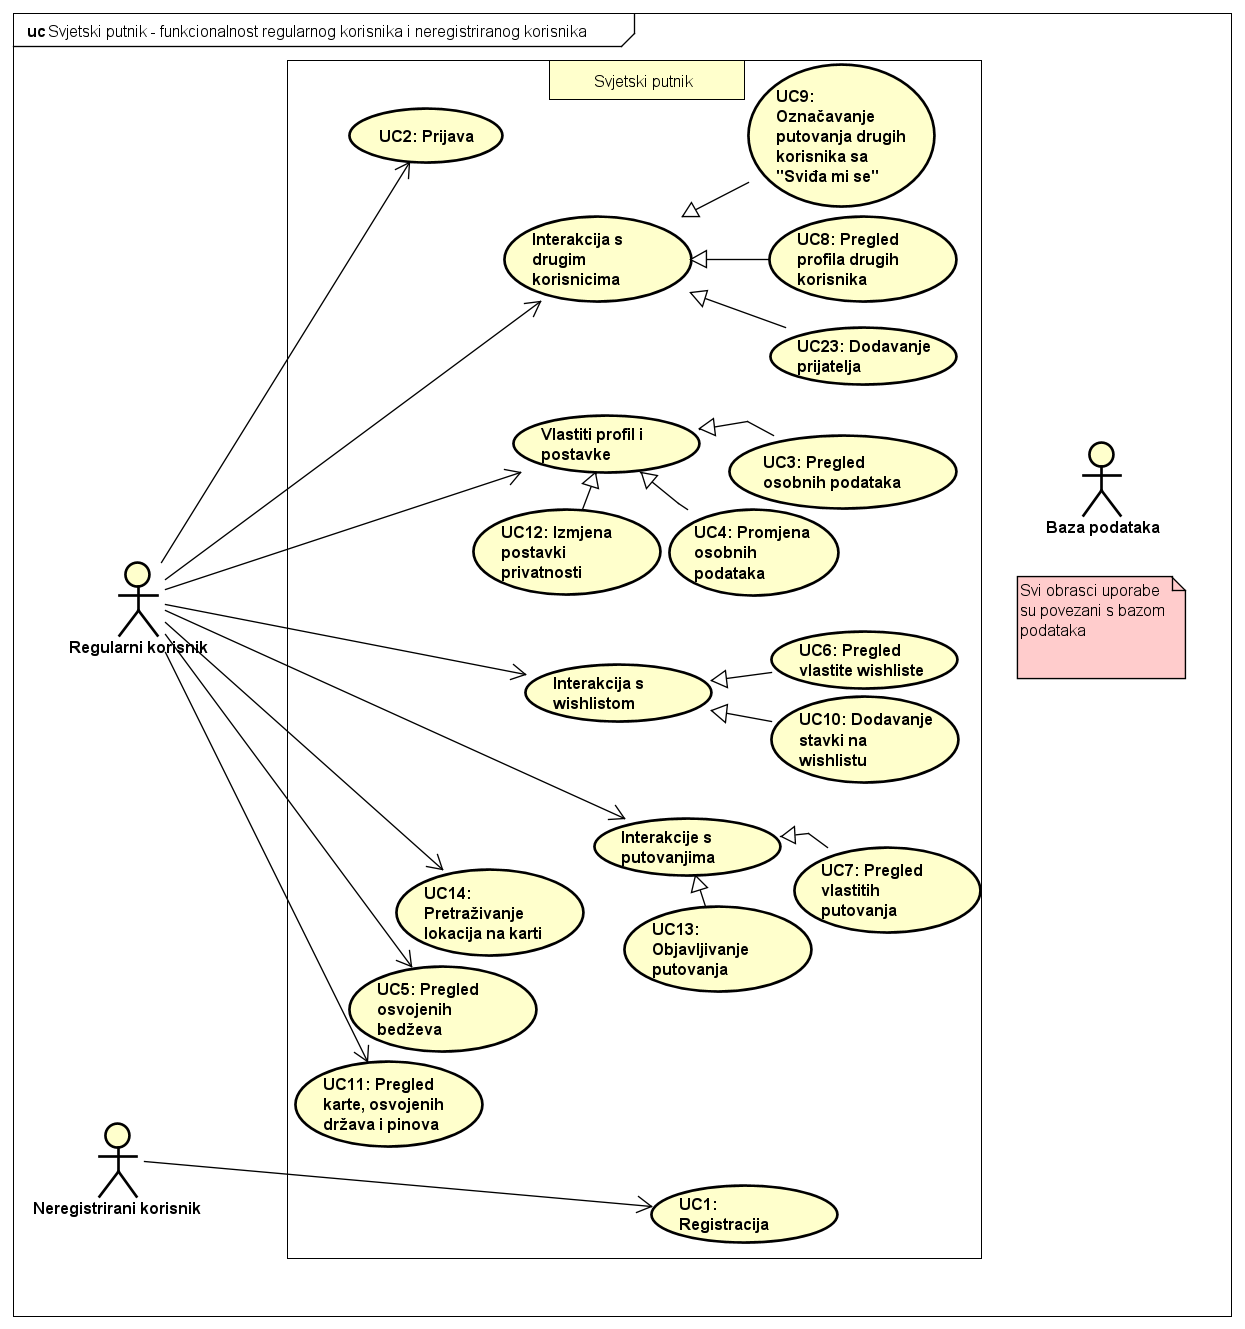
\includegraphics[scale=0.4]{slike/UC-regularnikorisnik-alt.png} %veličina slike u odnosu na originalnu datoteku i pozicija slike
                			\centering
                			\caption{UML dijagram obrazaca uporabe - regularni korisnik}
                			
                		\end{figure}
                		
                		\begin{figure}[H]
                			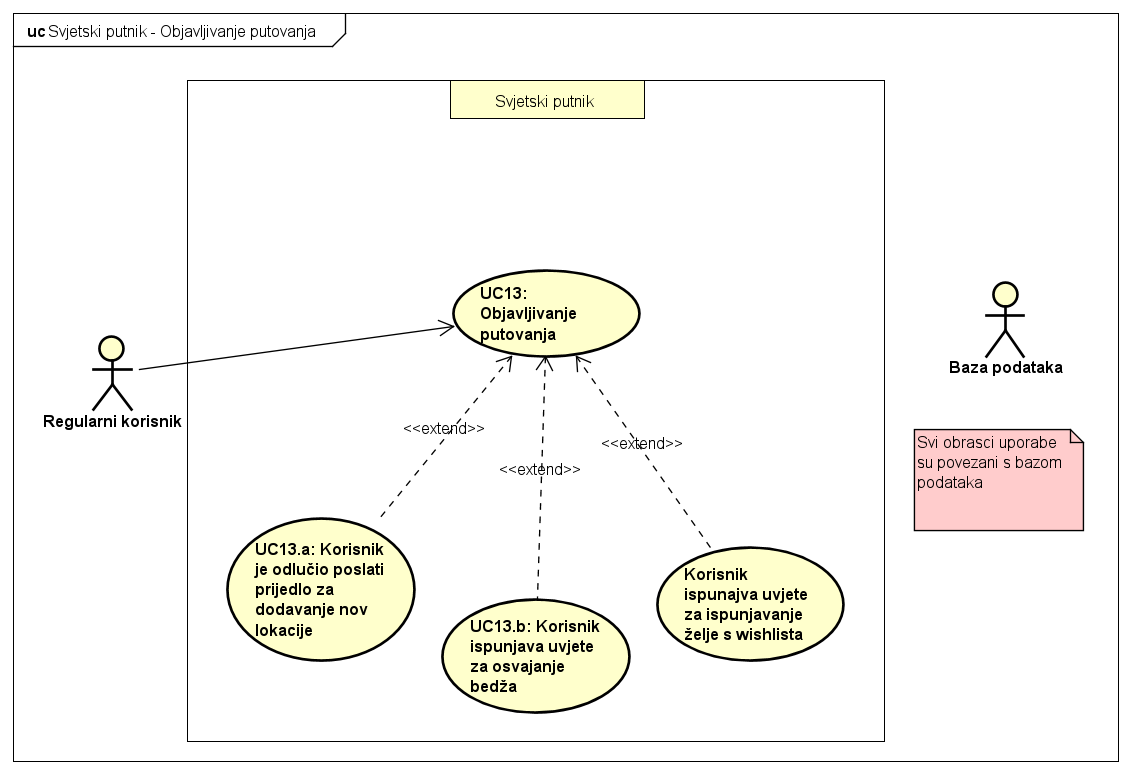
\includegraphics[scale=0.4]{slike/UC-objavljivanjeputovanja.png} %veličina slike u odnosu na originalnu datoteku i pozicija slike
                			\centering
                			\caption{UML dijagram obrazaca uporabe - objavljivanje putovanja}
                			
                		\end{figure}
        			
        				\begin{figure}[H]
                			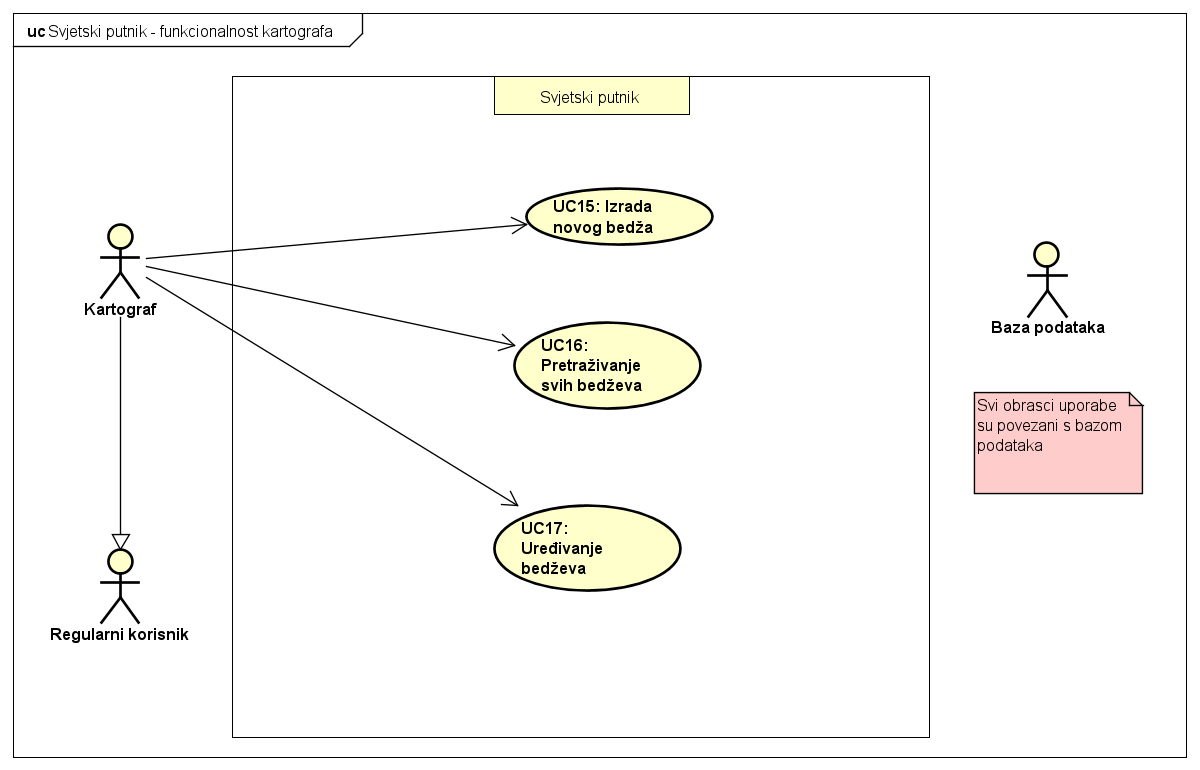
\includegraphics[scale=0.4]{slike/UC-kartograf.png} %veličina slike u odnosu na originalnu datoteku i pozicija slike
                			\centering
                			\caption{UML dijagram obrazaca uporabe - kartograf}
                			
                		\end{figure}
        			
        				\begin{figure}[H]
                			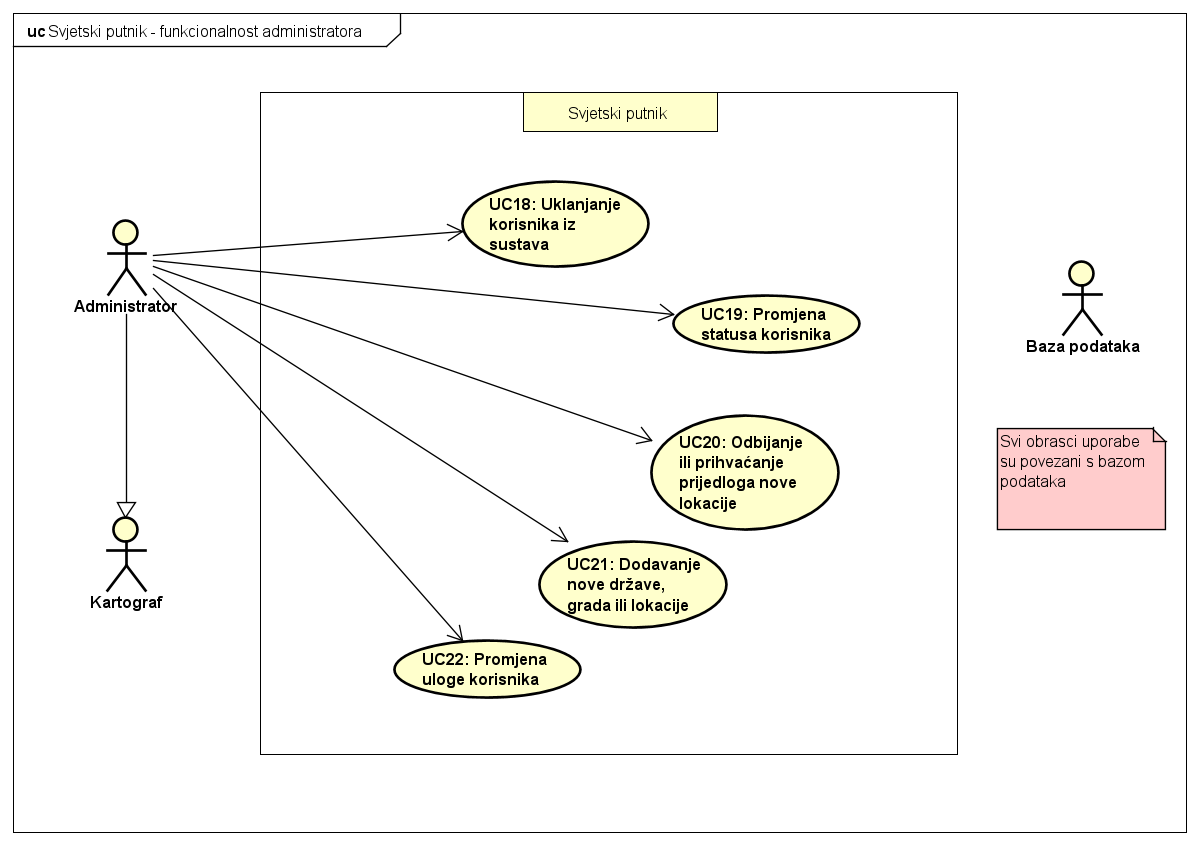
\includegraphics[scale=0.4]{slike/UC-dministrator.png} %veličina slike u odnosu na originalnu datoteku i pozicija slike
                			\centering
                			\caption{UML dijagram obrazaca uporabe - administrator}
                			
                		\end{figure}
				\eject		
				
			\subsection{Sekvencijski dijagrami}
			
			
			    Kartograf pristupa stranici "Bedževi", aplikacija prikazuje navedenu stranicu, Kartograf odabire "Novi Bedž", aplikacija prikazuje formu za kreiranje bedža. Kartograf ispunjava formu i šalje ispunjenu formu, aplikacija dodaje bedž u bazu podataka i kartografu prikazuje stranicu "Bedževi" (s vidljivim novim bedžem).
				\begin{figure}[H]
                	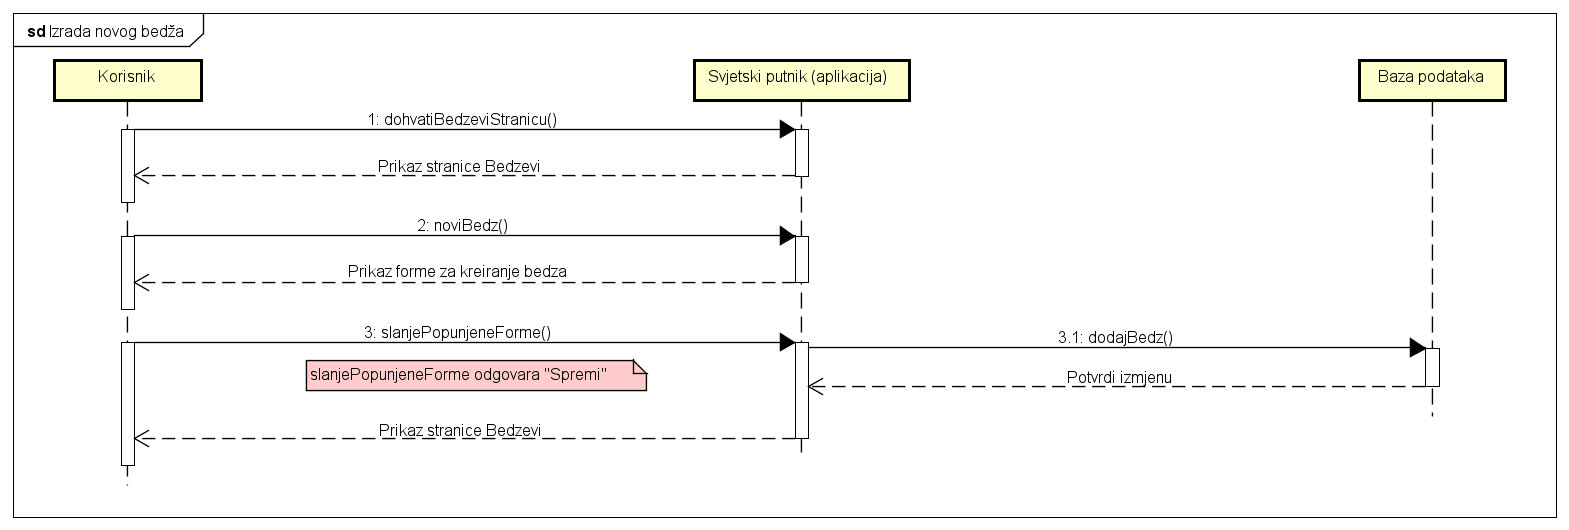
\includegraphics[scale=0.4]{slike/SD-izradabedza.png} %veličina slike u odnosu na originalnu datoteku i pozicija slike
                	\centering
                	\caption{UML sekvencijski dijagram - Izrada novog bedža}
                			
                \end{figure}
                
                
                Korisnik pristupa naslovnoj stranici, aplikacija dohvaća putovanja korisnika iz baze podataka te boja države i postavlja pinove na kartu. Aplikacija korisniku prikazuje naslovnicu sa obojenom kartom i pinovima.
                \begin{figure}[H]
                	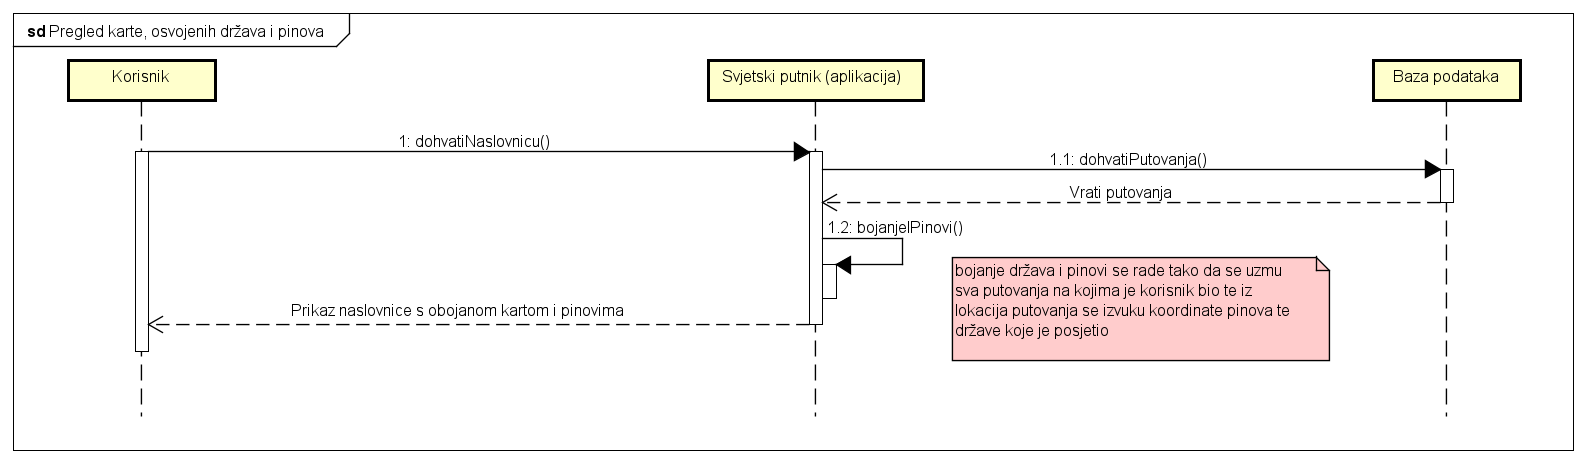
\includegraphics[scale=0.4]{slike/SD-pregledkarte.png} %veličina slike u odnosu na originalnu datoteku i pozicija slike
                	\centering
                	\caption{UML sekvencijski dijagram - Pregled karte, osvojenih država i pinova}
                			
                \end{figure}
                
                
                Korisnik odabire opciju "Nova objava", aplikacija korisniku prikazuje formu za izradu nove objave. Korisnik zatraži prikaz karte, aplikacija iz baze podataka dohvaća lokacije te prikazuje korisniku kartu s lokacijama. Korisnik ispunjava formu i označuje lokaciju. Korisnik šalje formu aplikaciji, aplikacija provjerava formu i ako lokacija ne postoji u bazi podataka sprema lokaciju (s flagom is\_suggestion). Aplikacija u bazu podataka sprema putovanje. Aplikacija dohvaća trenutne bedževe korisnika iz baze podataka i provjerava je li korisnik ispunio sva pravila za bilo koji bedž, ako je u bazi podataka se sprema osvojen bedž i uklanja trenutni bedž. Aplikacija dohvaća trenutnu wishlistu korisnika iz baze podataka i provjerava je li korisnik ispunjava uvjete bilo koje wishlist stavke, ako ispunjava u bazi podataka se sprema osvojen bedž i uklanja trenutni bedž. Aplikacija ponovno prikazuje stranicu bez forme s novim putovanjem dodanim.
                \begin{figure}[H]
                	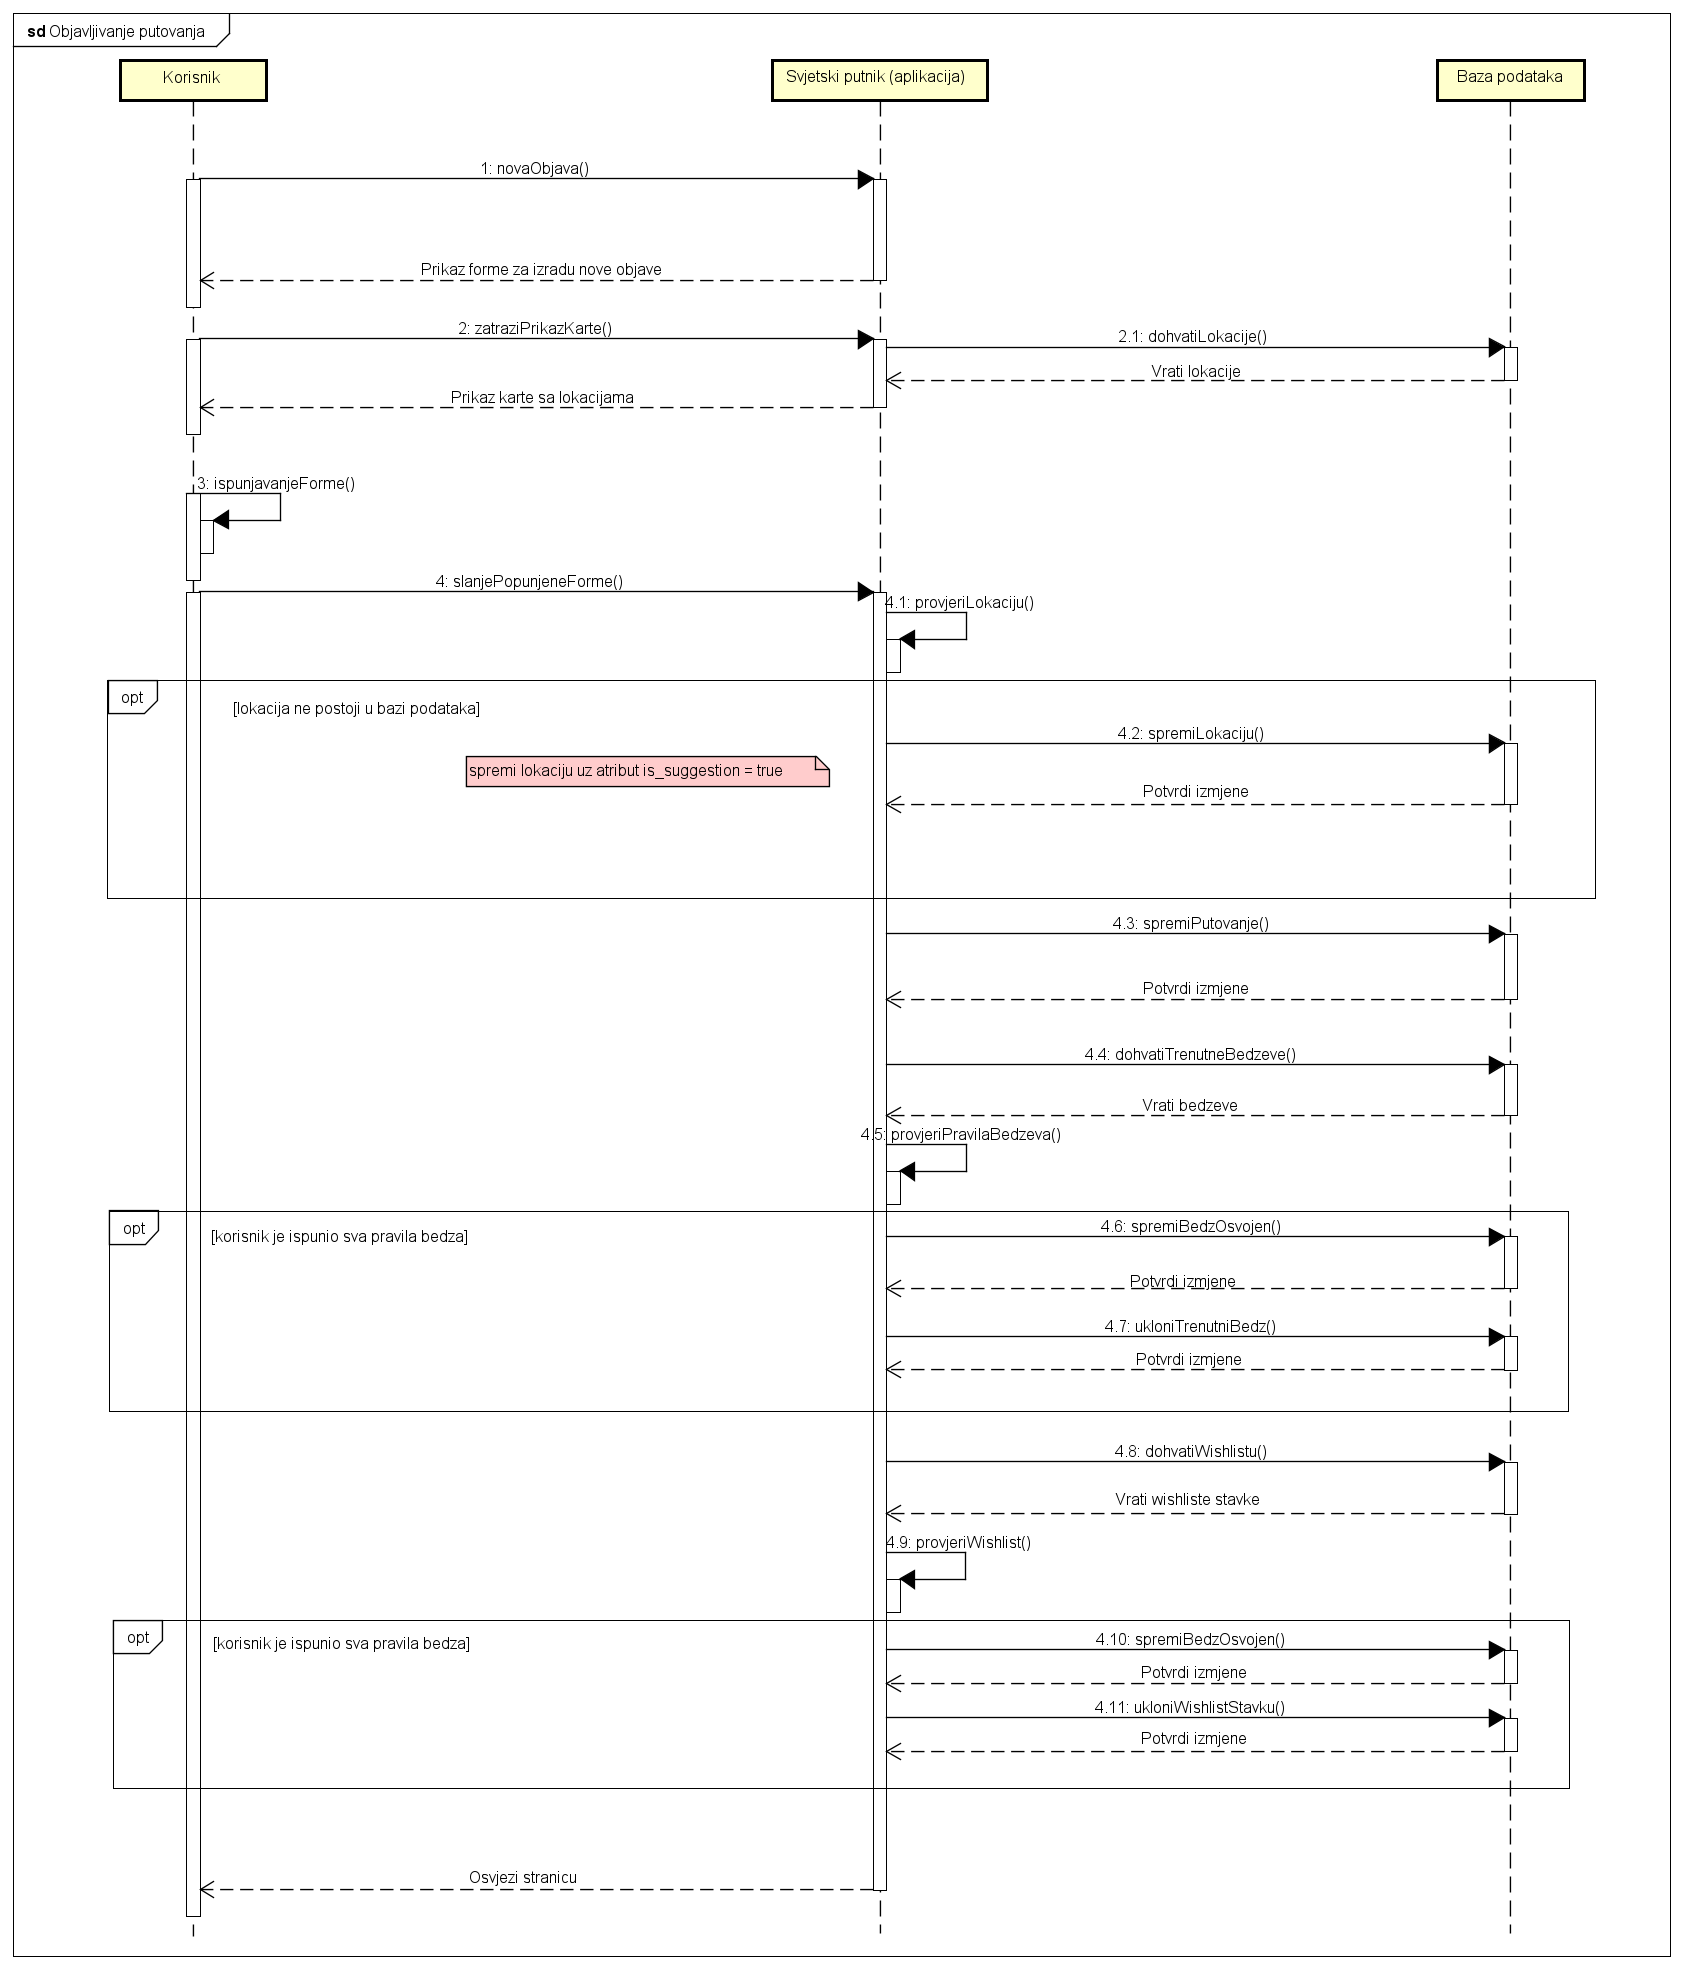
\includegraphics[scale=0.4]{slike/SD-objavljivanjeputovanja.png} %veličina slike u odnosu na originalnu datoteku i pozicija slike
                	\centering
                	\caption{UML sekvencijski dijagram - Objavljivanje putovanja}
                			
                \end{figure}
                
                
                Administrator odabire "Preporuke/prijedlozi (lokacija)", aplikacija dohvaća lokacije iz baze podataka, odabire one s flagom is\_suggestion i prikazuje ih Administratoru. Ako administrator smatra da je lokacija prihvatljiva onda prihvaća prijedlog te aplikacija ažurira u bazi podataka da je to prava lokacija, aplikacija prikazuje stranicu "Preporuke/prijedlozi (lokacija)". Ako administrator smatra da lokacije nije prihvatljiva onda odbija prijedlog te aplikacija uklanja lokaciju iz baze podataka te aplikacija prikazuje stranicu "Preporuke/prijedlozi (lokacija)".
                \begin{figure}[H]
                	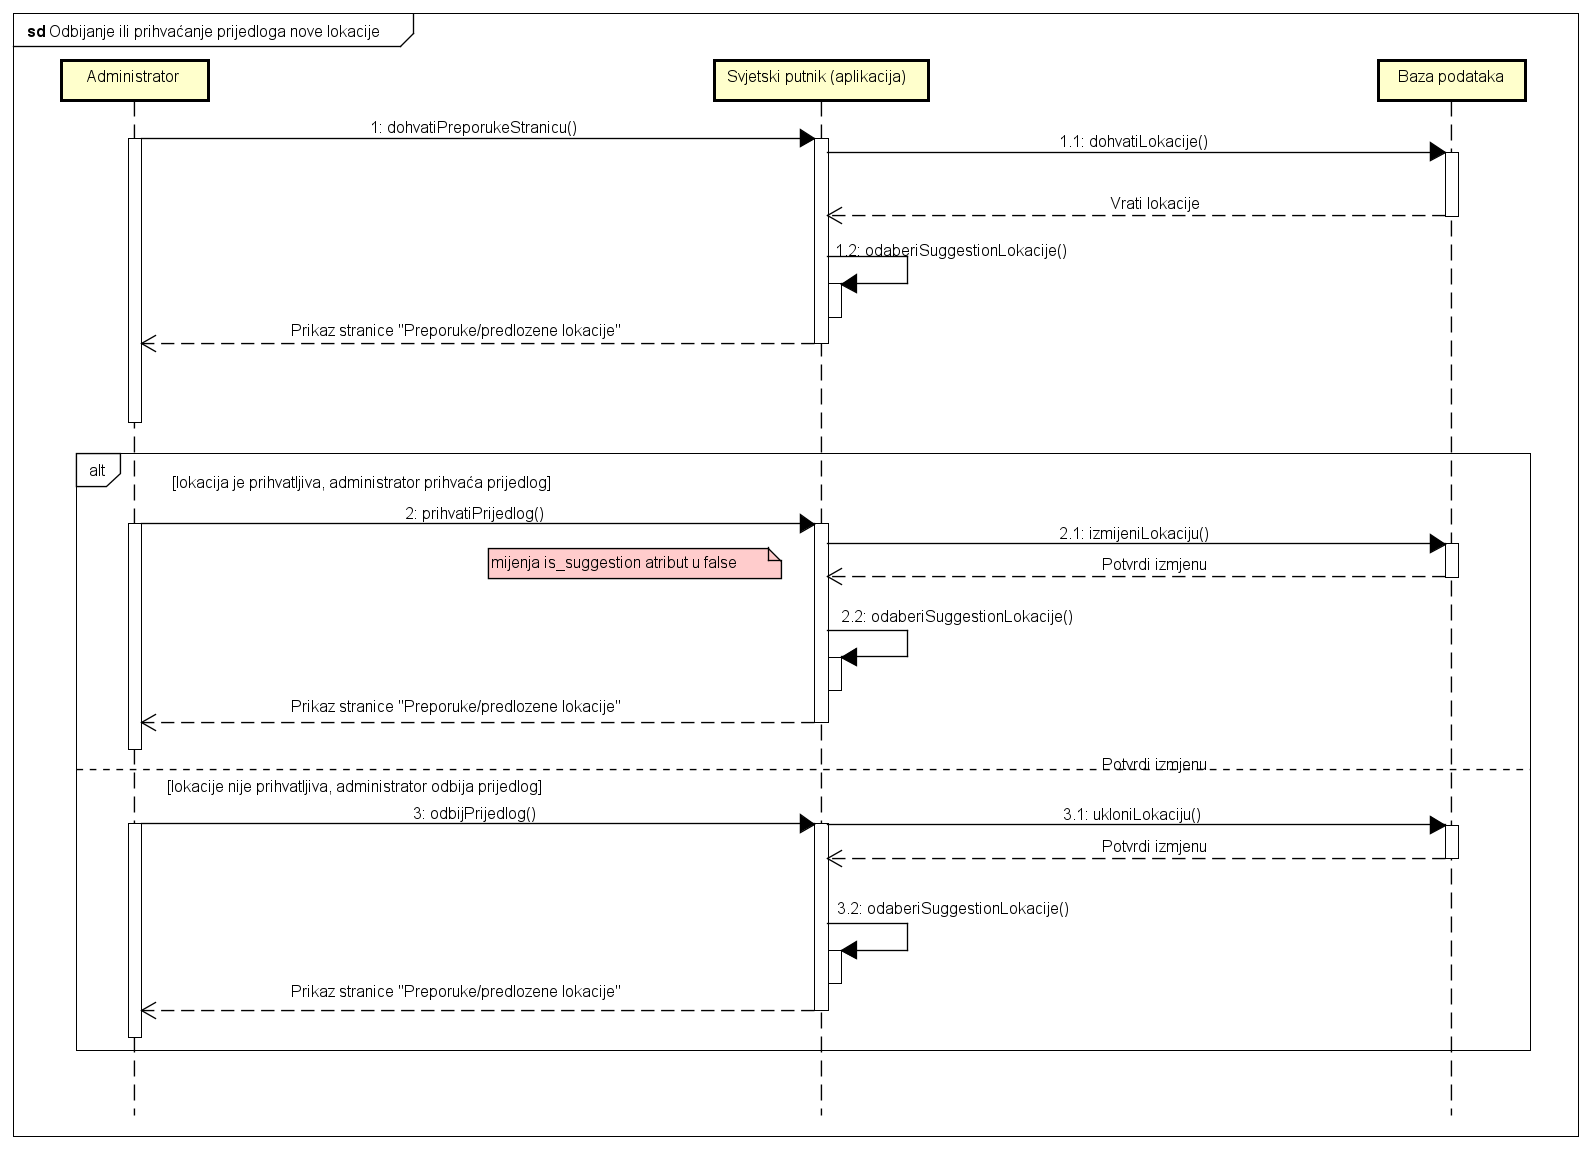
\includegraphics[scale=0.4]{slike/SD-odbijanjeprihvacanje.png} %veličina slike u odnosu na originalnu datoteku i pozicija slike
                	\centering
                	\caption{UML sekvencijski dijagram - Odbijanje ili prihvaćanje prijedloga nove lokacije}
                			
                \end{figure}
                
				
				\eject
	
		\section{Ostali zahtjevi}
		
		    
			\begin{packed_item}
			    \item Sustav treba omogućiti rad više korisnika u stvarnom vremenu
			    \item Neispravno korištenje korisničkog sučelja ne smije naručiti funkcionalnost sustava
			    \item Sustav mora biti jednostavan za korištenje
			    \item Veza prema bazi podataka treba biti zaštićena i brza
			    \item Korisničko sučelje mora podržavati hrvatsku abecedu pri unosu i prikazu tekstualnog sadržaja
			\end{packed_item}
			 
			 
			 
	
	\chapter{Arhitektura i dizajn sustava}

\begin{packed_item}
			\item Struktura:
			\begin{packed_enum}
				\item Web poslužitelj
				\item \textit{Frontend} aplikacija
				\item \textit{Backend} aplikacija
				\item Baza podataka
			\end{packed_enum}
			\item REST stil web servisa
			\item ORM (objektno-relacijsko preslikavanje)
			\item Relacijska baza podataka
			\item \textit{Clean} arhitektura \textit{Backend}-a
		\end{packed_item}


		\textit{Web preglednik} je program pomoću kojeg korisnik može pristupati resursima na internetu. Ima ulogu klijenta koji traži resurse od dostupnih poslužitelja. U ovom slučaju, korisnik putem preglednika šalje zahtjev za dohvaćanje \textit{(Frontend) web aplikacije}, koja je implementirana kao \textit{SPA (engl. Single Page Application)} - statički servirana web stranica s dinamičkim kretanjem po sadržaju ovisno o putanji, bez obaveznog osvježavanja stranice.


		\textit{Frontend} (korisnička) aplikacija služi za komunikaciju s \textit{Backend} aplikacijom na poslužitelju, gdje se sva bitna poslovna logika aplikacije nalazi, a to omogućuje kroz korisničko sučelje.


		\textit{Backend} aplikacija prima korisničke zahtjeve i obrađuje ih, ovisno o zahtjevu korisnika pristupa bazi podataka te šalje potvrdne ili neuspješne odgovore prema korisničkoj aplikaciji, po potrebi i s dodatnim podacima u tijelu odgovora.

		\eject

		\section{Programski jezici, razvojni okviri, alati i biblioteke koda}

		\subsection{\textit{Backend} i baza podataka}
		U \textit{Backend} aplikaciji koristi se Java, Spring boot, JPA, Liquibase, PostgreSQL, XML, YAML, Gradle te JWT autentikacija/autorizacija.


		Spring boot je Java \textit{Framework} koji olakšava izradu web aplikacije kroz automatsku konfiguraciju ovisnih dijelova aplikacije unutar projekta te pruža razne implementacije tih dijelova koje apstrahiraju korištenje kroz intuitivna sučelja.


		\textit{Liquibase} se koristi za definiranje sheme baze podataka. JPA služi za preslikavanje entiteta iz \textit{PostgreSQL} baze podataka na klase u \textit{Backend} aplikaciji, a time se postiže lakše generiranje upita ovisno o pozivu metode na klasi entiteta.



		YAML je format datoteke korišten za konfiguracijske datoteke aplikacije, a XML za datoteke dnevnika promjena (engl. changelog). Za upravljanje bazom podataka koristi se DBeaver, a za realizaciju \textit{Backend} aplikacije Jetbrains IntelliJ Idea (Java). Za izgradnju cijele aplikacije koristi se Gradle, a za sigurnost se koristi \textit{JWT (engl. Json Web Token)} standard za generiranje tokena koji istovremeno služe za autorizaciju i autentikaciju korisnika.


		\subsection{\textit{Frontend}}
		Za \textit{Frontend} aplikaciju koristi se Typescript, React, TailwindCSS, Vite, React Query, Formik, HeadlessUI te Figma.


		React je \textit{Framework} koji olakšava izradu web stranica kroz razne implementacije za navigaciju, dohvaćanje te prikaz podataka. Za definiranje sadržaja stranice koristi označni kod sličan HTML-u, proširen mogućnostima Typescript-a. Za definiranje stila tj. izgleda stranice koristi se TailwindCSS.


		React Query koristi se za raspodjelu podataka u aplikaciji, za izradu formi koristi se biblioteka Formik, a za ponašanje kompleksnijih komponenti na stranici HeadlessUI. Vite je alat korišten za izgradnju cijele aplikacije.


		Dizajn ekrana aplikacije odrađen je pomoću alata Figma, a pisanje Typescripta u Visual Studio Code-u.







		\eject


		\section{Baza podataka}

		    Baza podataka korištena u projektu je PostgreSQL. 

			\subsection{Opis tablica}

				Trip - opisuje jedno objavljeno putovanje korisnika. U \textit{one to many} vezi s Location, \textit{many to one} sa User\_profile.

				\begin{longtblr}[
					label=none,
					entry=none
					]{
						width = \textwidth,
						colspec={|X[10,l]|X[6, l]|X[20, l]|},
						rowhead = 1,
					} %definicija širine tablice, širine stupaca, poravnanje i broja redaka naslova tablice
					\hline \multicolumn{3}{|c|}{\textbf{Trip}}	 \\ \hline[3pt]
					\SetCell{LightGreen}id & INT	&  	primarni ključ relacije Trip  	\\ \hline
					\SetCell{LightBlue}\textbf{user\_id}	& INT &  strani ključ od relacije User\_profile (User\_profile.user\_id) 	\\ \hline
					\SetCell{LightBlue}\textbf{location\_id} & INT &  strani ključ od relacije Location (Location.id)\\ \hline
					date\_visited & TIMESTAMP	&  	datum putovanja	\\ \hline
					upload\_timestamp & TIMESTAMP	&  	datum objave putovanja	\\ \hline
					transportation\_type & VARCHAR	&  	tip prijevoza	\\ \hline
					traffic\_rating & VARCHAR	&  	ocjena gužve na putovanju \\ \hline
					is\_solo & BOOLEAN	&  	samostalno ili putovanje u društvu	\\ \hline
					trip\_rating & VARCHAR	&  	ocjena putovanja	\\ \hline
					description & VARCHAR	&  	komentar na putovanje	\\ \hline
                        image & BYTEA & slika putovanja  \\ \hline
					%\SetCell{LightBlue} primjer	& VARCHAR &   	\\ \hline
				\end{longtblr}

				Trip\_like je veza \textit{many to many} između User\_profile i Trip.
				\begin{longtblr}[
					label=none,
					entry=none
					]{
						width = \textwidth,
						colspec={|X[10,l]|X[6, l]|X[20, l]|},
						rowhead = 1,
					}
					\hline \multicolumn{3}{|c|}{\textbf{Trip\_like}}	 \\ \hline[3pt]
					\SetCell{LightGreen}\textbf{user\_id} & INT	&  	primarni ključ relacije Trip\_like i strani ključ od relacije User\_profile (User\_profile.user\_id)	\\ \hline
					\SetCell{LightGreen}\textbf{trip\_id} & INT	&  	primarni ključ relacije Trip\_like i strani ključ od relacije Trip (Trip.id)	\\ \hline
					%\SetCell{LightBlue} primjer	& VARCHAR &   	\\ \hline
				\end{longtblr}

				Location - opisuje jednu lokaciju na karti. U \textit{one to many} vezi s Trip, \textit{many to one} vezi s City, \textit{one to many} sa Wishlist\_entry i \textit{many to one} s Account.
				\begin{longtblr}[
					label=none,
					entry=none
					]{
						width = \textwidth,
						colspec={|X[10,l]|X[6, l]|X[20, l]|},
						rowhead = 1,
					}
					%1:N trip
					%N:1 city
					%1:N wishlist entry
				    %N:N:N loc:userprf:badge
				    %N:1 account suggestioni
					\hline \multicolumn{3}{|c|}{\textbf{Location}}	 \\ \hline[3pt]
					\SetCell{LightGreen}id & INT	&  	  primarni ključ relacije Location  	\\ \hline
					name & VARCHAR	&  	ime lokacije	\\ \hline
					x\_coordinate	& INT &  x koordinata lokacije 	\\ \hline
					y\_coordinate & INT &  y koordinata lokacije \\ \hline
					type & VARCHAR	&  	tip lokacije (muzej, crkva...)	\\ \hline
					\SetCell{LightBlue}\textbf{city\_id} & INT &  strani ključ od relacije City (City.id)  \\ \hline
					is\_suggestion & BOOLEAN	&  	je li lokacija prijedlog regularnog korisnika	\\ \hline
					\SetCell{LightBlue}\textbf{suggested\_by\_user\_id}  & INT & strani ključ od relacije Account (Account.id)  \\ \hline
					%\SetCell{LightBlue} primjer	& VARCHAR &   	\\ \hline
				\end{longtblr}

				City - opisuje jedan grad. U \textit{one to many} vezi s Location i \textit{many to one} vezi s Country.
				\begin{longtblr}[
					label=none,
					entry=none
					]{
						width = \textwidth,
						colspec={|X[10,l]|X[6, l]|X[20, l]|},
						rowhead = 1,
					}
					%1:N loc
					%N:1 country
					\hline \multicolumn{3}{|c|}{\textbf{City}}	 \\ \hline[3pt]
					\SetCell{LightGreen}id & INT	&  	primarni ključ relacije City 	\\ \hline
					name & VARCHAR	&  ime grada		\\ \hline
					\SetCell{LightBlue}\textbf{country\_code} & INT &  strani ključ od relacije Country (Country.code)\\ \hline
					%\SetCell{LightBlue} primjer	& VARCHAR &   	\\ \hline
				\end{longtblr}

				Country - opisuje jednu državu. U \textit{one to many} vezi s City.
				\begin{longtblr}[
					label=none,
					entry=none
					]{
						width = \textwidth,
						colspec={|X[10,l]|X[6, l]|X[20, l]|},
						rowhead = 1,
					}
					%1:N city
					\hline \multicolumn{3}{|c|}{\textbf{Country}}	 \\ \hline[3pt]
					\SetCell{LightGreen}id & INT	&  	primarni ključ relacije Country 	\\ \hline
					name & VARCHAR	&  	ime države	\\ \hline
					%\SetCell{LightBlue} primjer	& VARCHAR &   	\\ \hline
				\end{longtblr}

				Wishlist\_entry - jedna želja na popisu želja. U \textit{many to one} vezi s Location, \textit{many to one} sa User\_profile te \textit{one to one} vezi s Badge.
				\begin{longtblr}[
					label=none,
					entry=none
					]{
						width = \textwidth,
						colspec={|X[10,l]|X[6, l]|X[20, l]|},
						rowhead = 1,
					}
					%N:1 lokacija
					%N:1 userpf
					%1:1 wishl badg
					\hline \multicolumn{3}{|c|}{\textbf{Wishlist\_entry}}	 \\ \hline[3pt]
					\SetCell{LightGreen}id & INT	&  	primarni ključ relacije Wishlist\_entry 	\\ \hline
					\SetCell{LightBlue}\textbf{user\_id} & INT &   strani ključ od relacije User\_profile (User\_profile.user\_id) \\ \hline
					\SetCell{LightBlue}\textbf{location\_id} & INT &   strani ključ od relacije Location (Location.id)\\ \hline
					visit\_before & TIMESTAMP &  deadline kada želja treba biti ispunjena  \\ \hline
					state & VARCHAR	&  	stanje	\\ \hline
					%\SetCell{LightBlue} primjer	& VARCHAR &   	\\ \hline
				\end{longtblr}

				Wishlist\_badge je veza između entiteta. \textit{One to one} veza Wishlist\_entry i Badge.
				\begin{longtblr}[
					label=none,
					entry=none
					]{
						width = \textwidth,
						colspec={|X[10,l]|X[6, l]|X[20, l]|},
						rowhead = 1,
					}
					%1:1 wishlist etny
					%0..1:1 badge
					\hline \multicolumn{3}{|c|}{\textbf{Wishlist\_badge}}	 \\ \hline[3pt]
					\SetCell{LightGreen}\textbf{id} & INT	&  	primarni ključ relacije Wishlist\_badge i strani ključ od relacije Badge 	\\ \hline
					\SetCell{LightBlue}\textbf{wishlist\_entry\_id} & INT &   strani ključ od relacije Wishlist\_entry (Wishlist\_entry.id) \\ \hline
					%\SetCell{LightBlue} primjer	& VARCHAR &   	\\ \hline
				\end{longtblr}

				Won\_badge je veza \textit{many to many to many} Location, User\_profile, Badge.
				\begin{longtblr}[
					label=none,
					entry=none
					]{
						width = \textwidth,
						colspec={|X[10,l]|X[6, l]|X[20, l]|},
						rowhead = 1,
					}

					\hline \multicolumn{3}{|c|}{\textbf{Won\_badge}}	 \\ \hline[3pt]
					\SetCell{LightGreen}\textbf{user\_id} & INT	&  	primarni ključ relacije Won\_badge i strani ključ od relacije User\_profile (User\_profile.user\_id)	\\ \hline
					\SetCell{LightGreen}\textbf{badge\_id} & INT & primarni i strani ključ od relacije Badge (Badge.id) \\ \hline
					\SetCell{LightGreen}\textbf{last\_location\_id} & INT & primarni i strani ključ od relacije Location (Location.id) \\ \hline
					won\_timestamp & TIMESTAMP & datum osvajanja bedža   \\ \hline
					%\SetCell{LightBlue} primjer	& VARCHAR &   	\\ \hline
				\end{longtblr}

				Badge - opisuje jedan bedž. U \textit{one to one} vezi s City\_badge i \textit{one to one} vezi s Country\_badge.
				\begin{longtblr}[
					label=none,
					entry=none
					]{
						width = \textwidth,
						colspec={|X[10,l]|X[6, l]|X[20, l]|},
						rowhead = 1,
					}
					%1:0..1 wish bacge
					%1:0..1 ctry bdg
					%1:0..1 city bdg
					%N:N:N loc:userprf:badge
					\hline \multicolumn{3}{|c|}{\textbf{Badge}}	 \\ \hline[3pt]
					\SetCell{LightGreen}id & INT	&  	primarni ključ relacije Badge 	\\ \hline
					name & VARCHAR	&  	ime bedža	\\ \hline
					image & INT &   slika bedža  \\ \hline
					type & VARCHAR	&  	tip bedža	\\ \hline
                        image & BYTEA & slika bedža  \\ \hline
					%\SetCell{LightBlue} primjer	& VARCHAR &   	\\ \hline
				\end{longtblr}

				City\_badge - opisuje pravila za gradove. U \textit{one to one} vezi s Badge i \textit{one to many} vezi s City\_badge\_requirement.
				\begin{longtblr}[
					label=none,
					entry=none
					]{
						width = \textwidth,
						colspec={|X[10,l]|X[6, l]|X[20, l]|},
						rowhead = 1,
					}
					%0..1:1 badge
					%1:N city badge req
					\hline \multicolumn{3}{|c|}{\textbf{City\_badge}}	 \\ \hline[3pt]
					\SetCell{LightGreen}\textbf{id} & INT	&  primarni relacije City i strani ključ od relacije Badge (Badge.id)	\\ \hline
					required\_locations & INT &  broj koliko minimalno lokacija unutar grada treba posjetiti  \\ \hline
					%\SetCell{LightBlue} primjer	& VARCHAR &   	\\ \hline
				\end{longtblr}

				City\_badge\_requirement - opisuje pravila lokacija unutar grada. U \textit{many to one} vezi s City\_badge.
				\begin{longtblr}[
					label=none,
					entry=none
					]{
						width = \textwidth,
						colspec={|X[10,l]|X[6, l]|X[20, l]|},
						rowhead = 1,
					}
					%N:1 city bdg
					\hline \multicolumn{3}{|c|}{\textbf{City\_badge\_requirement}}	 \\ \hline[3pt]
					\SetCell{LightGreen}id & INT	&  primarni	ključ relacije City\_badge\_requirement 	\\ \hline
					\SetCell{LightBlue}\textbf{badge\_id} & INT &   strani ključ od relacije City\_badge (City\_badge.id)\\ \hline
					required\_locations & INT &  broj koliko minimalno lokacija tipa \textbf{location\_type} unutar grada treba posjetiti   \\ \hline
					location\_type & VARCHAR	&  	tip lokacije	\\ \hline
					%\SetCell{LightBlue} primjer	& VARCHAR &   	\\ \hline
				\end{longtblr}

				Country\_badge - opisuje pravila za države. U \textit{one to one} vezi s Badge.
				\begin{longtblr}[
					label=none,
					entry=none
					]{
						width = \textwidth,
						colspec={|X[10,l]|X[6, l]|X[20, l]|},
						rowhead = 1,
					}
					%0..1:1 badge
					\hline \multicolumn{3}{|c|}{\textbf{Country\_badge}}	 \\ \hline[3pt]
					\SetCell{LightGreen}\textbf{id} & INT	&  primarni ključ relacije Country\_badge i strani ključ relacije od relacije Badge (Badge.id)	\\ \hline
					visit\_capital\_city & BOOLEAN &  je li potrebno posjetiti glavni grad  \\ \hline
					required\_number & INT &  ako je potrebno posjetiti glavni grad, broj \textbf{type} koje je potrebno posjetiti izvan glavnog grad. ako nije potrebno posjetiti glavni grad, broj \textbf{type} koje je potrebno posjetiti unutar države\\ \hline
					type & VARCHAR	&  enumeracija: grad, lokacija	\\ \hline
					%\SetCell{LightBlue} primjer	& VARCHAR &   	\\ \hline
				\end{longtblr}

				Account - opisuje jedan korisnički račun. U \textit{one to one} vezi sa User\_profile i \textit{one to many} vezi s Location.
				\begin{longtblr}[
					label=none,
					entry=none
					]{
						width = \textwidth,
						colspec={|X[10,l]|X[6, l]|X[20, l]|},
						rowhead = 1,
					}
					%1:1 usr pf
					%n:n role
					%1:n location
					\hline \multicolumn{3}{|c|}{\textbf{Account}}	 \\ \hline[3pt]
					\SetCell{LightGreen}id & INT	&  	primarni ključ relacije Account 	\\ \hline
					name & VARCHAR	&  	ime korisnika	\\ \hline
					surname & VARCHAR	&  	prezime korisnika	\\ \hline
					username & VARCHAR	&  	korisničko ime korisnika	\\ \hline
					email & VARCHAR	&  	email korisnika	\\ \hline
				    password & VARCHAR	&  lozinka korisnika		\\ \hline
					is\_active & BOOLEAN &  je li korisnikov račun aktivan  \\ \hline
					%\SetCell{LightBlue} primjer	& VARCHAR &   	\\ \hline
				\end{longtblr}

				User\_profile - opisuje jedan korisnički profil. U \textit{one to one} vezi s Account, \textit{one to many} vezi sa Trip i \textit{one to many} vezi sa Wishlist\_entry.
				\begin{longtblr}[
					label=none,
					entry=none
					]{
						width = \textwidth,
						colspec={|X[10,l]|X[6, l]|X[20, l]|},
						rowhead = 1,
					}
					%n:n user pf firend
					%n:n trip (trip_like)
					%1:1 acc
					%1:n trip
					%:N:N loc:userprf:badge
					%1:n wishlist entry
					\hline \multicolumn{3}{|c|}{\textbf{User\_profile}}	 \\ \hline[3pt]
					\SetCell{LightGreen}\textbf{user\_id} & INT	& primarni ključ relacije User\_profile i strani ključ relacije od relacije Account (Account.id) 	\\ \hline
					is\_public & BOOLEAN &  je li profil javan, prikazuju li se putovanja  \\ \hline
					profile\_image & BYTEA & slika korisničkog profila  \\ \hline
					%\SetCell{LightBlue} primjer	& VARCHAR &   	\\ \hline
				\end{longtblr}

				Friend je veza \textit{many to many} između User\_profile i User\_profile.
				\begin{longtblr}[
					label=none,
					entry=none
					]{
						width = \textwidth,
						colspec={|X[10,l]|X[6, l]|X[20, l]|},
						rowhead = 1,
					}
					\hline \multicolumn{3}{|c|}{\textbf{Friend}}	 \\ \hline[3pt]
					\SetCell{LightGreen}\textbf{from\_user\_id} & INT	&  primarni ključ relacije Friend i strani ključ od relacije User\_profile (User\_profile.user\_id) \\ \hline
					\SetCell{LightGreen}\textbf{to\_user\_id} & INT	&  	primarni ključ relacije Friend i strani ključ od relacije User\_profile (User\_profile.user\_id)\\ \hline
					is\_trip\_friend & BOOLEAN &  je li prijatelj označeno kao prijatelj s putovanja  \\ \hline
					%\SetCell{LightBlue} primjer	& VARCHAR &   	\\ \hline
				\end{longtblr}

				User\_role je veza \textit{many to many} između Account i Role.
				\begin{longtblr}[
					label=none,
					entry=none
					]{
						width = \textwidth,
						colspec={|X[10,l]|X[6, l]|X[20, l]|},
						rowhead = 1,
					}
					\hline \multicolumn{3}{|c|}{\textbf{User\_role}}	 \\ \hline[3pt]
					\SetCell{LightGreen}\textbf{user\_id} & INT	&  	primarni ključ relacije User\_role i strani ključ od relacije Account \\ \hline
					\SetCell{LightGreen}\textbf{role\_id} & INT	&  	primarni ključ relacije User\_role i strani ključ od relacije Role \\ \hline
					%\SetCell{LightBlue} primjer	& VARCHAR &   	\\ \hline
				\end{longtblr}

				Role - opisuje jednu korisničku ulogu.
				\begin{longtblr}[
					label=none,
					entry=none
					]{
						width = \textwidth,
						colspec={|X[10,l]|X[6, l]|X[20, l]|},
						rowhead = 1,
					}
					%n:n account (user:_role)
					\hline \multicolumn{3}{|c|}{\textbf{Role}}	 \\ \hline[3pt]
					\SetCell{LightGreen}id & INT	&  primarni	ključ relacije Role \\ \hline
					name & VARCHAR & ime uloge\\ \hline
					%\SetCell{LightBlue} primjer	& VARCHAR &   	\\ \hline
				\end{longtblr}







			\subsection{Dijagram baze podataka}
				\begin{figure}[H]
        			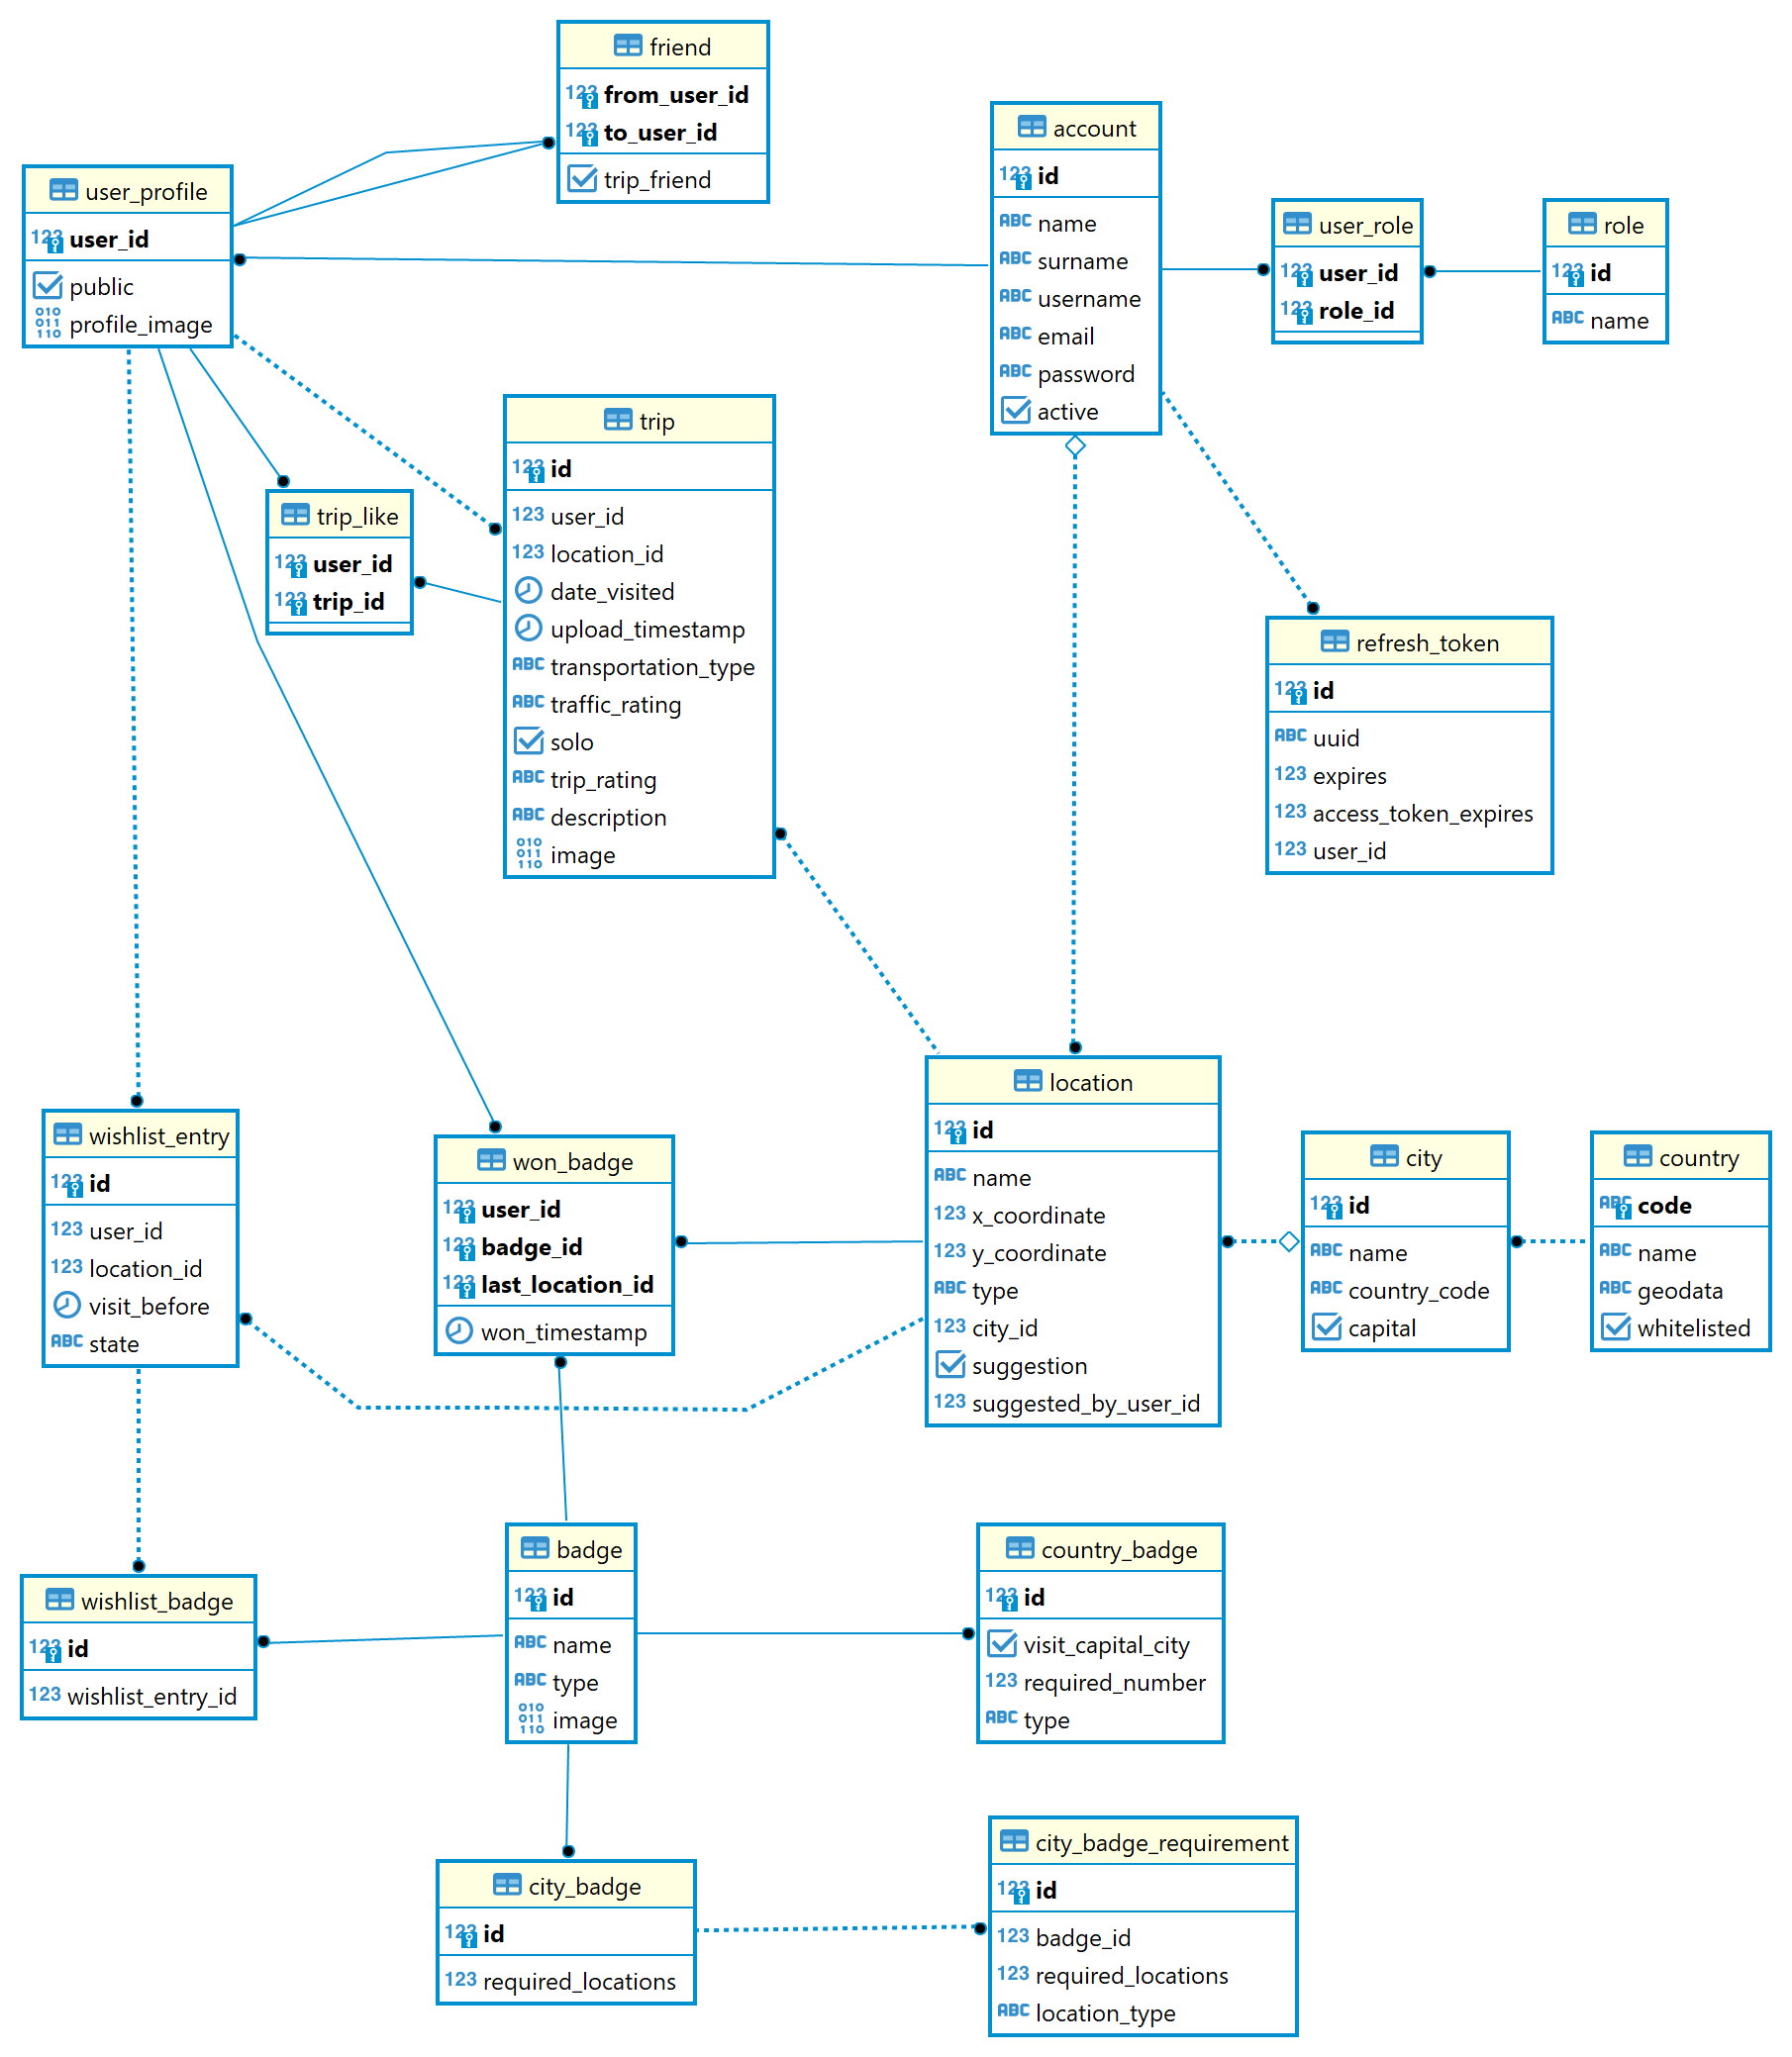
\includegraphics[scale=0.2]{slike/dijagram_baze.png} %veličina slike u odnosu na originalnu datoteku i pozicija slike
        			\centering
        			\caption{Dijagram baze podataka}

        		\end{figure}


		\section{Dijagram razreda}

                \begin{figure}[H]
        			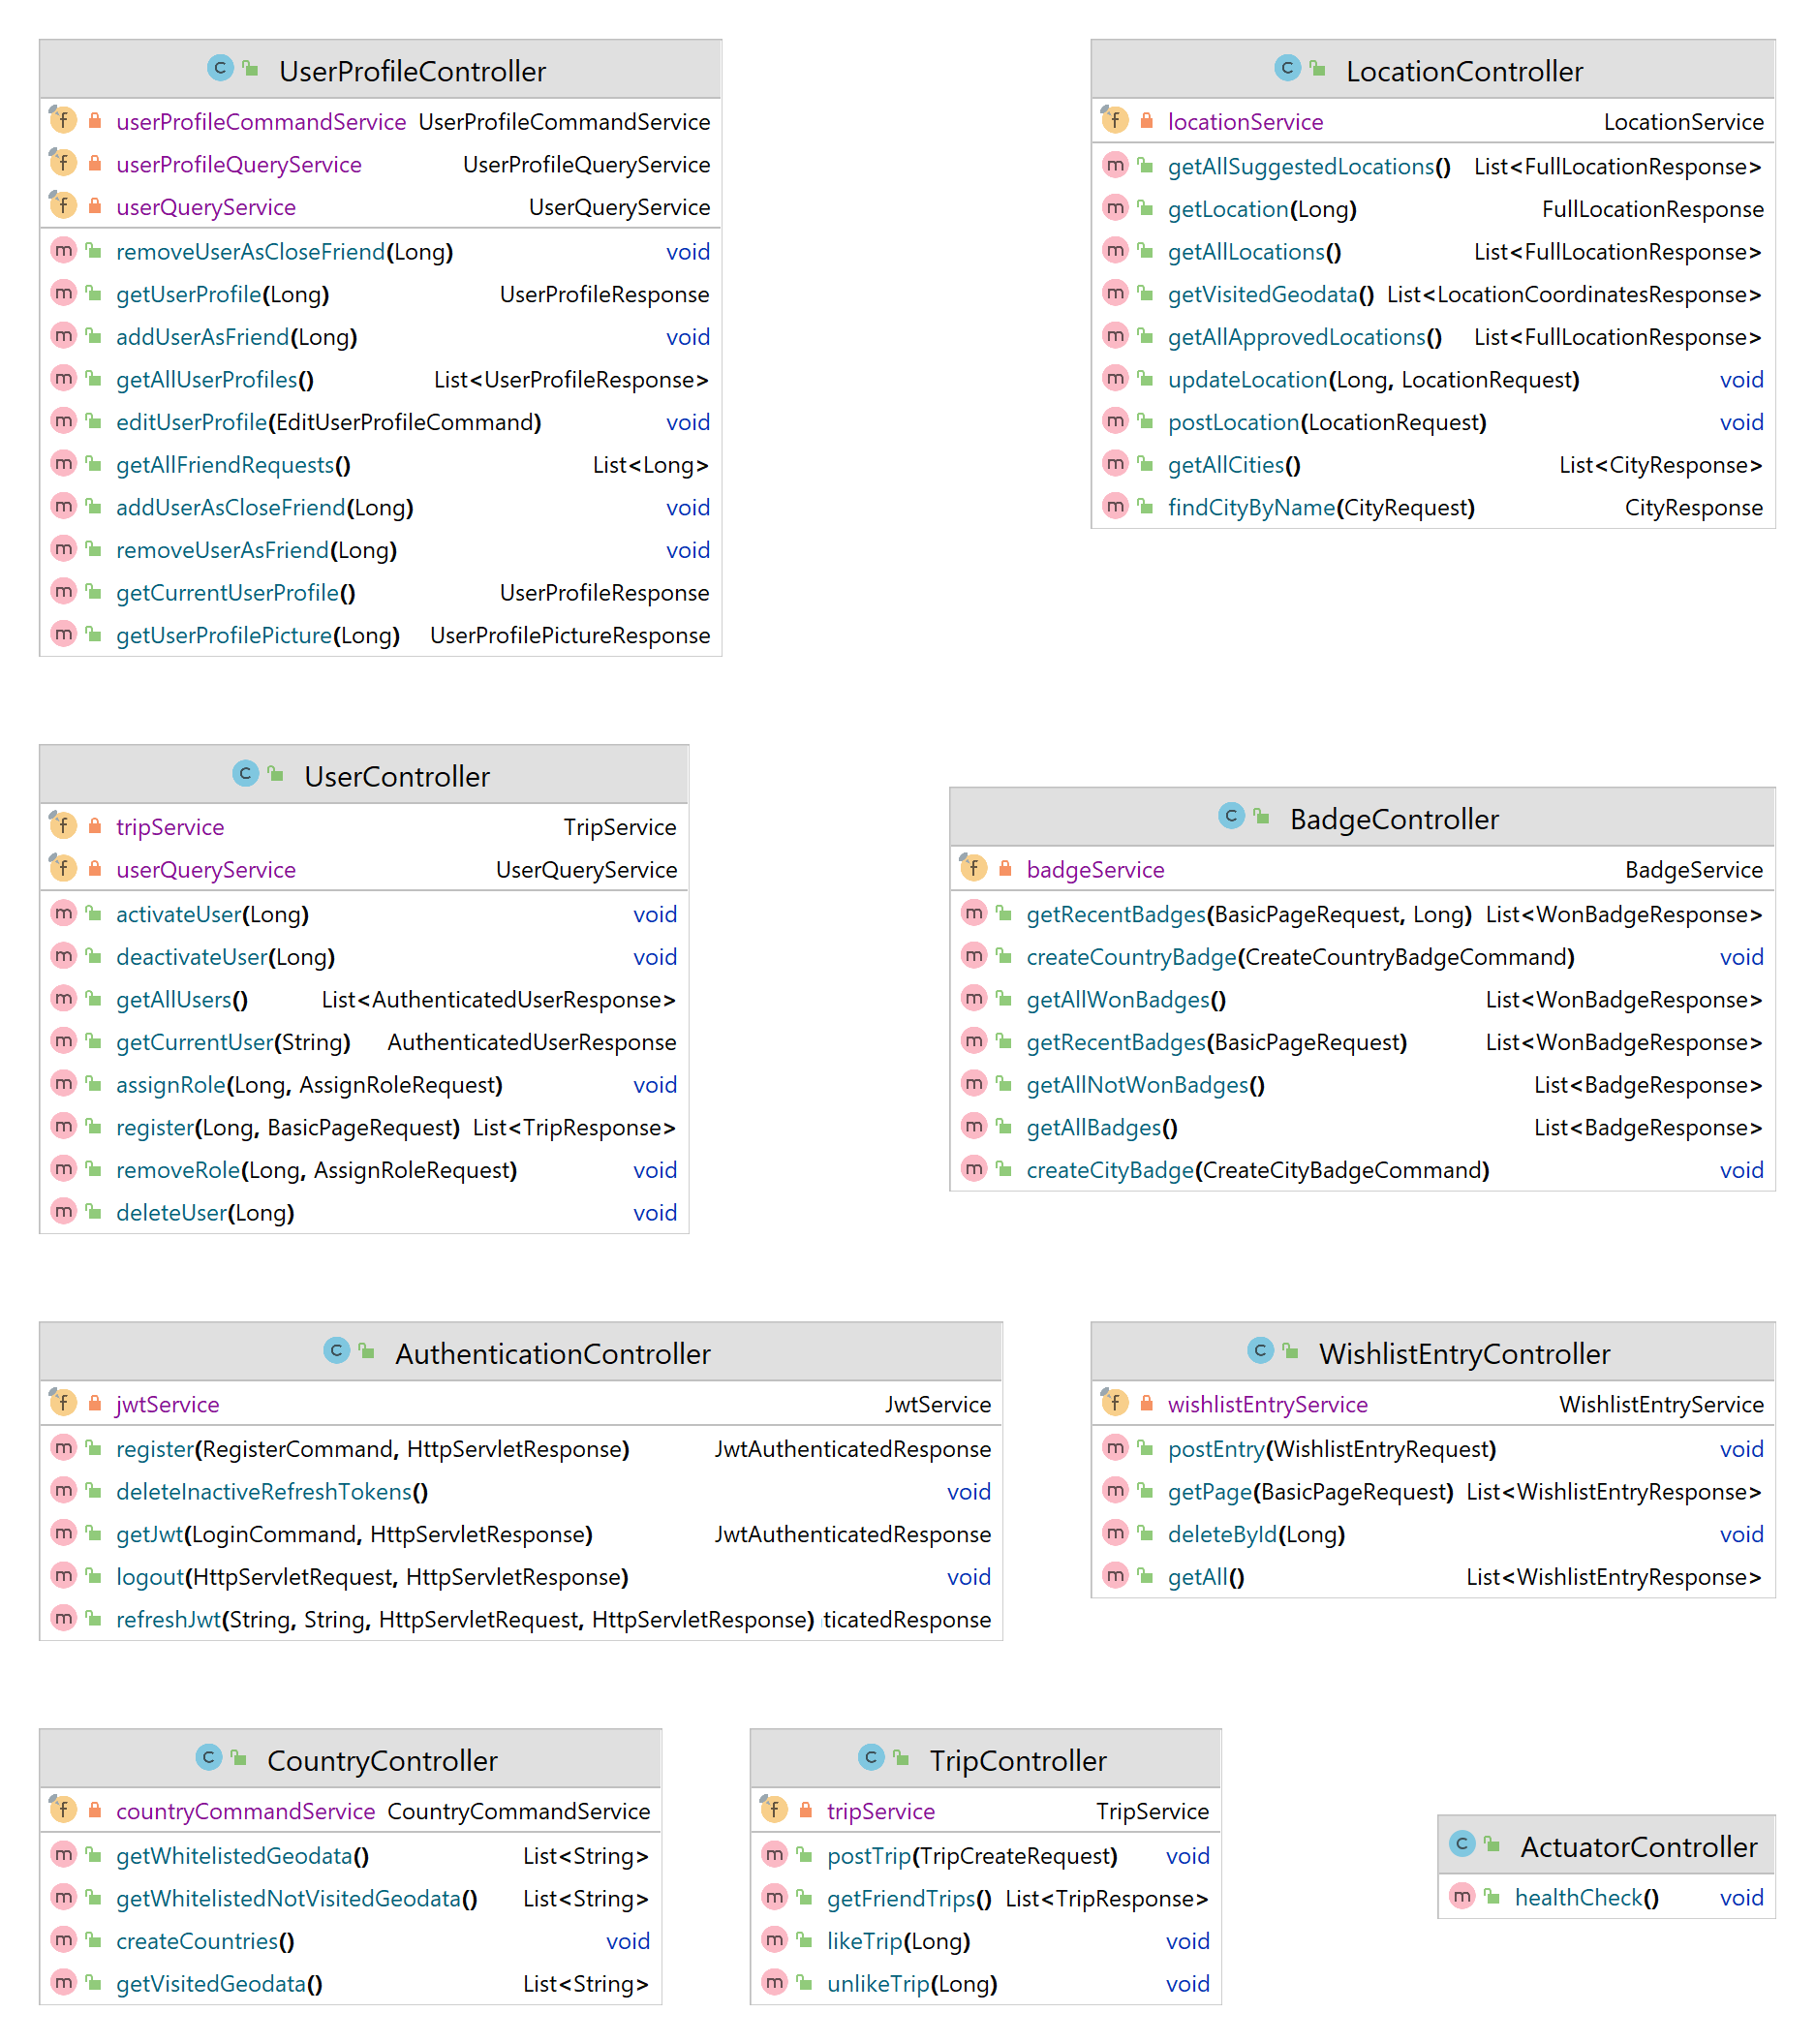
\includegraphics[scale=0.2]{slike/class/class_controller.png} %veličina slike u odnosu na originalnu datoteku i pozicija slike
        		\centering
        		\caption{Dijagram razreda - \textit{Controller}}

        	\end{figure}

                \begin{figure}[H]
        			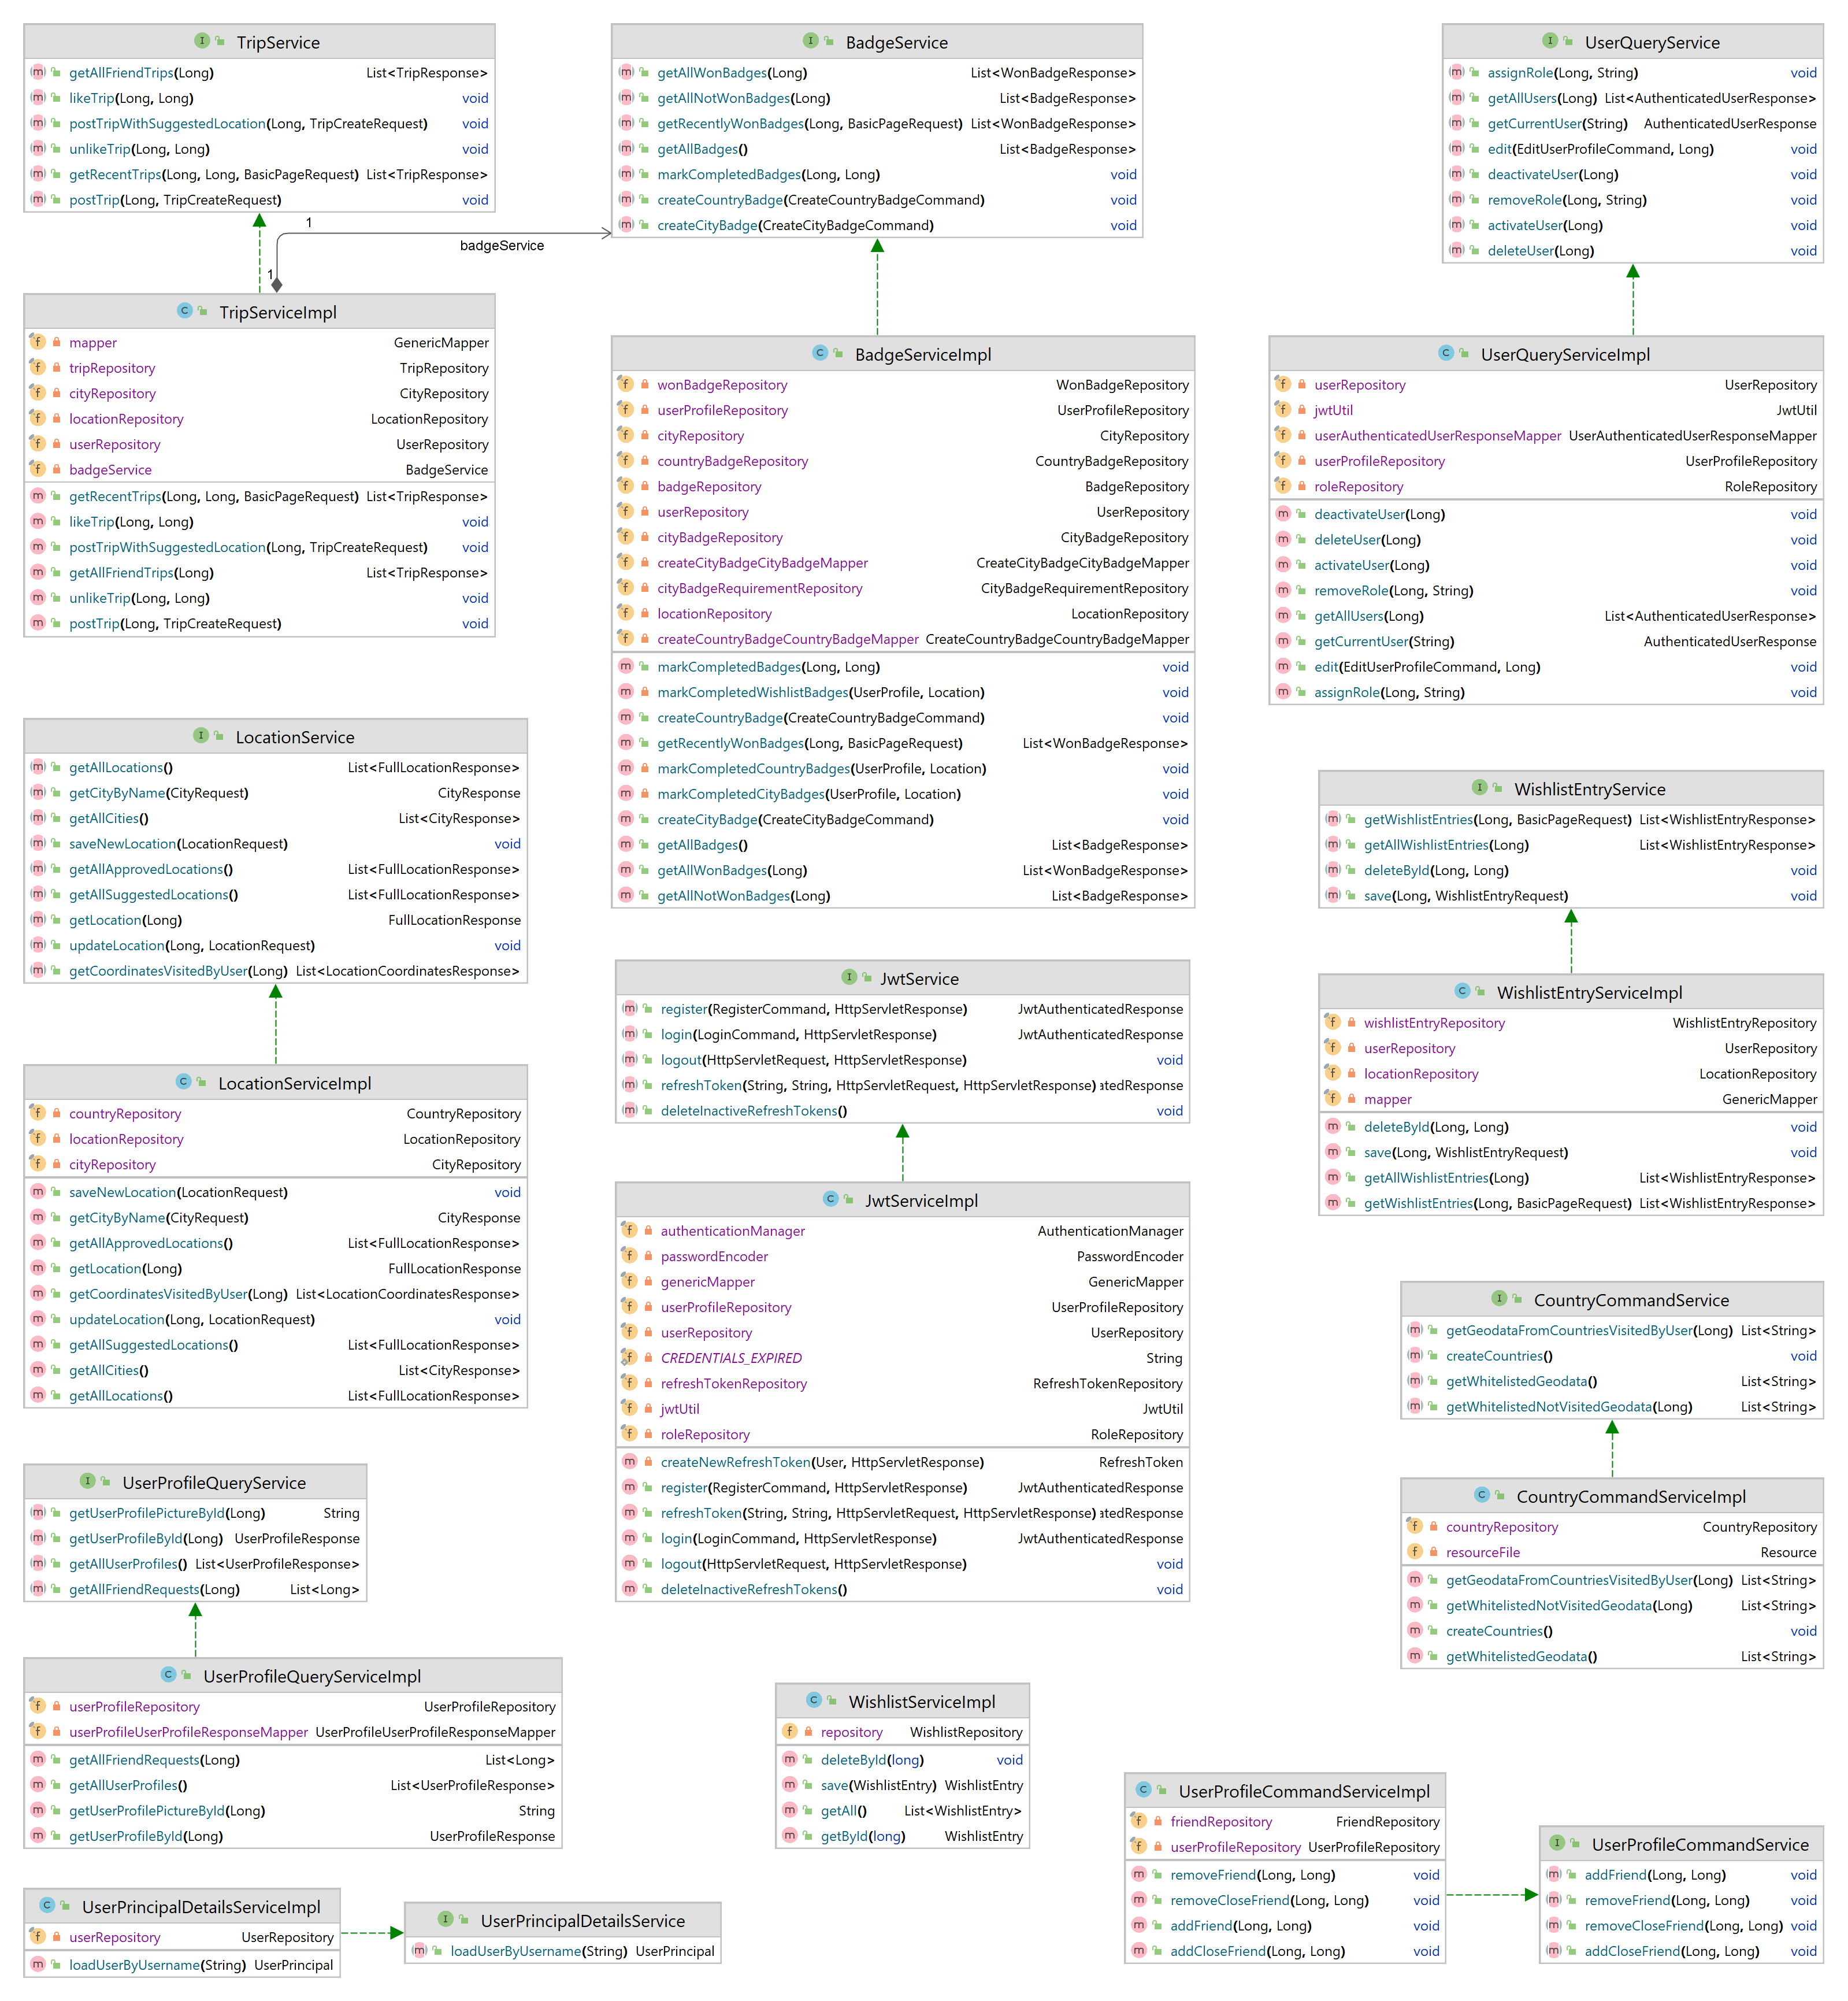
\includegraphics[scale=0.12]{slike/class/class_service.png} %veličina slike u odnosu na originalnu datoteku i pozicija slike
        		\centering
        		\caption{Dijagram razreda - \textit{Service}}
        	\end{figure}

                 \begin{figure}[H]
        			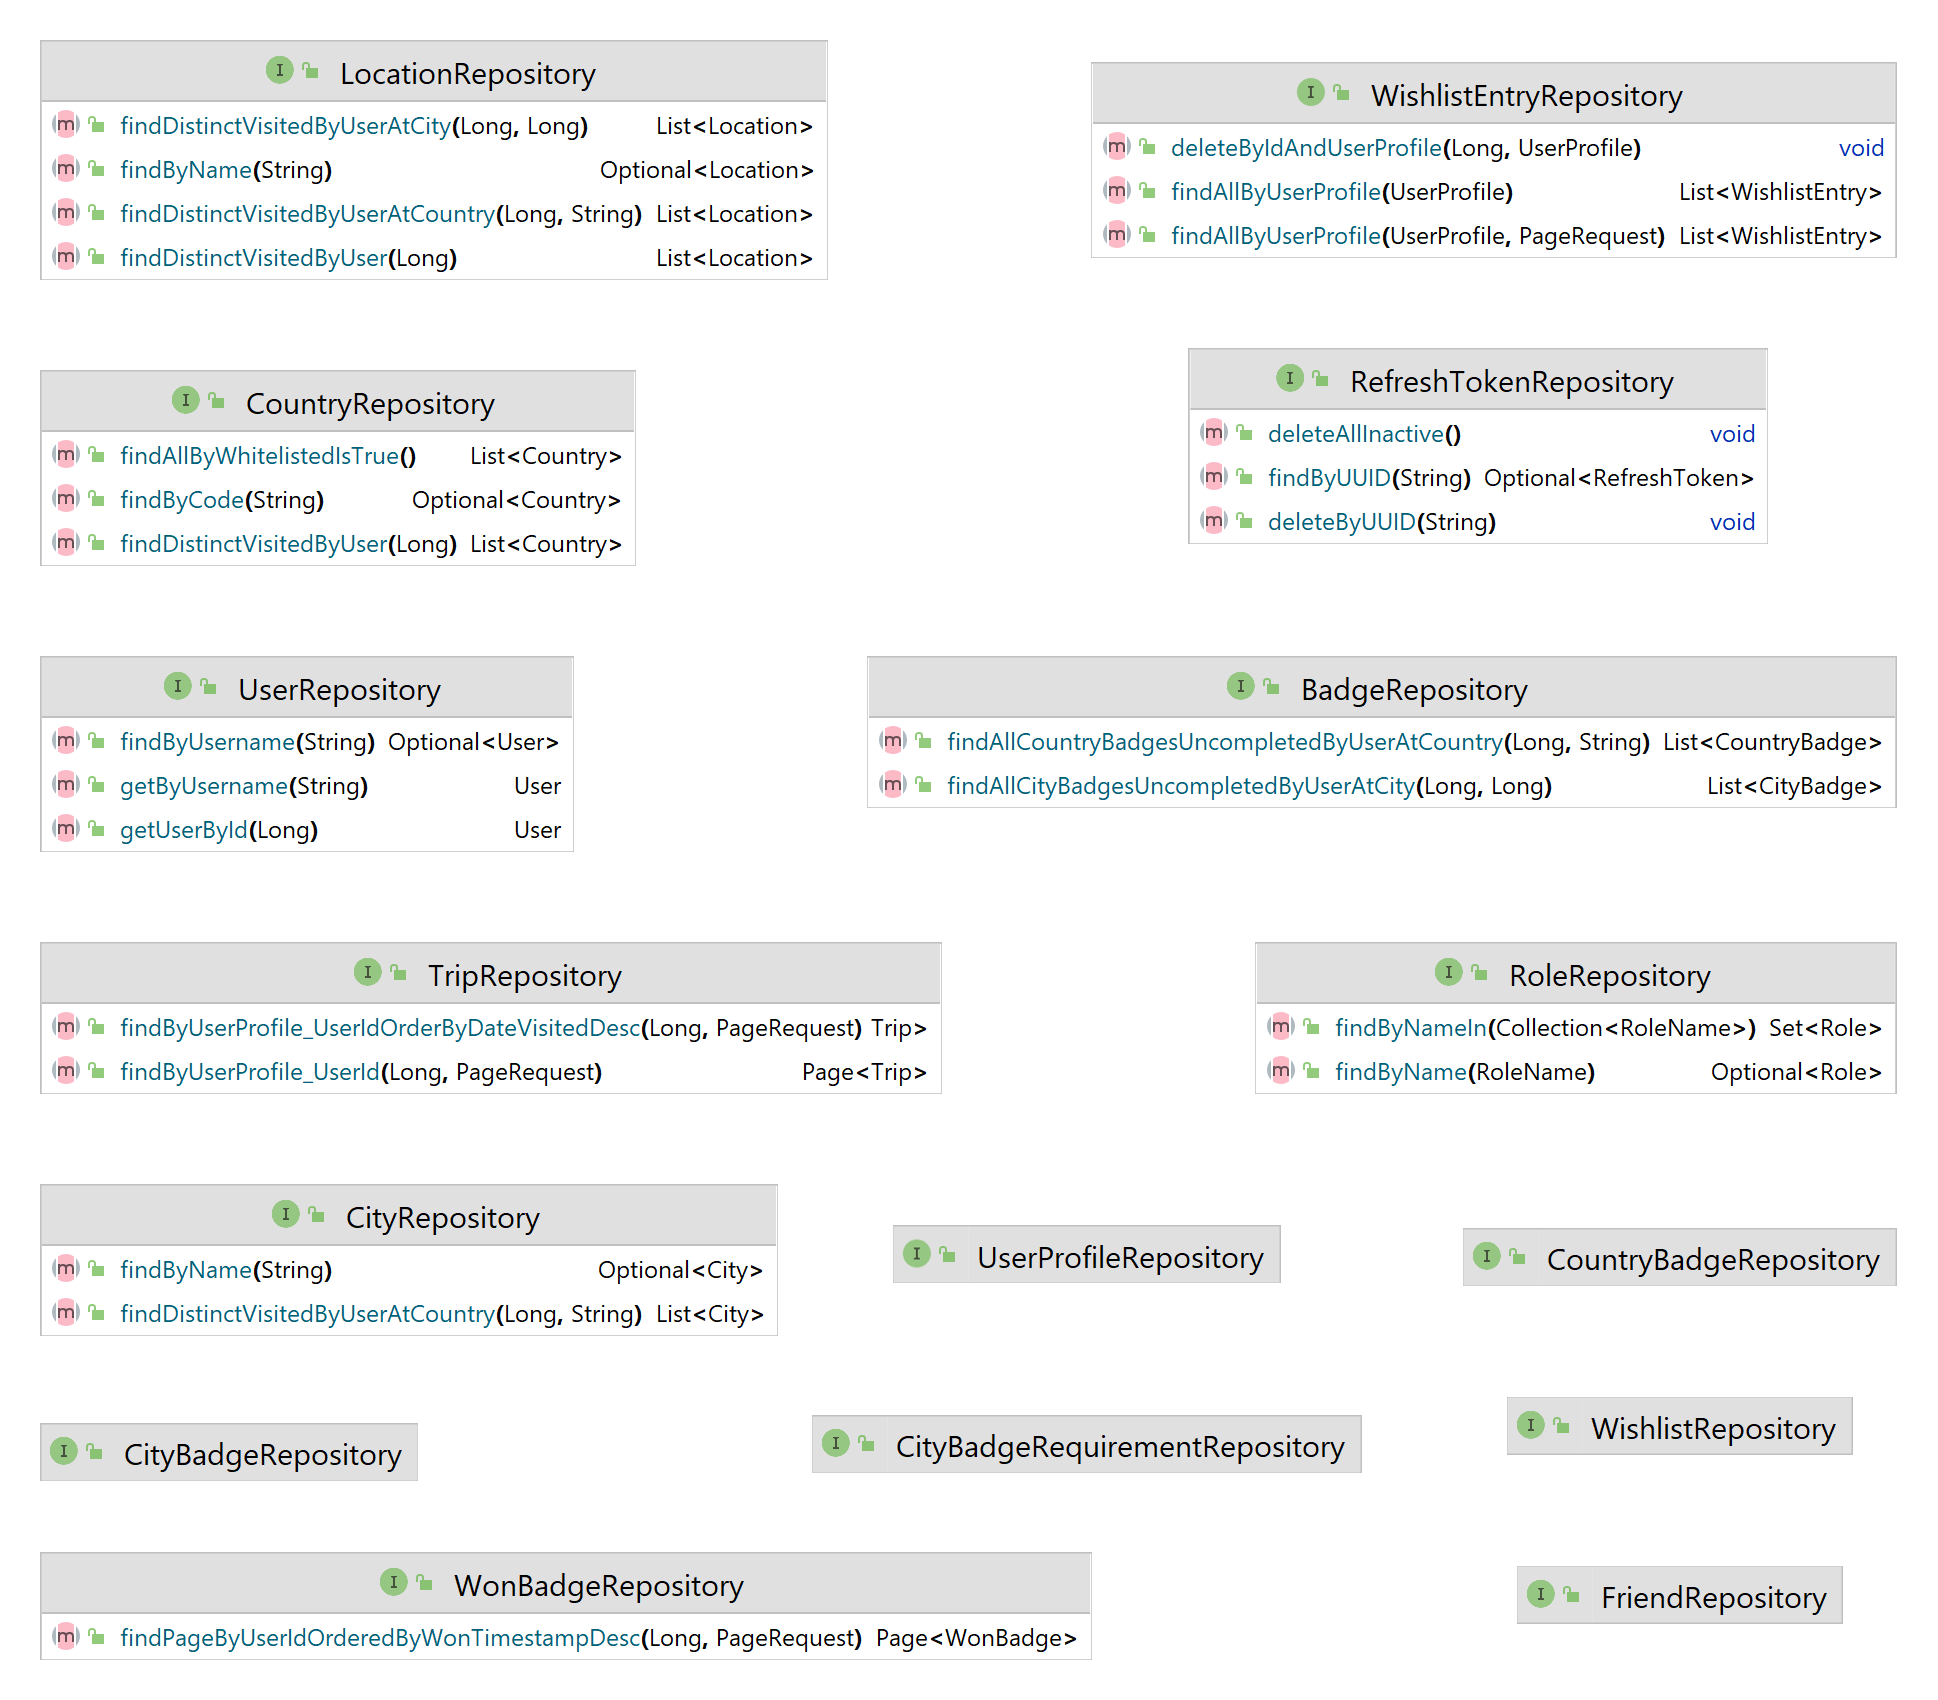
\includegraphics[scale=0.2]{slike/class/class_respository.png} %veličina slike u odnosu na originalnu datoteku i pozicija slike
        		\centering
        		\caption{Dijagram razreda - \textit{Repository}}

        	\end{figure}
                \eject
        
                \begin{figure}[H]
        			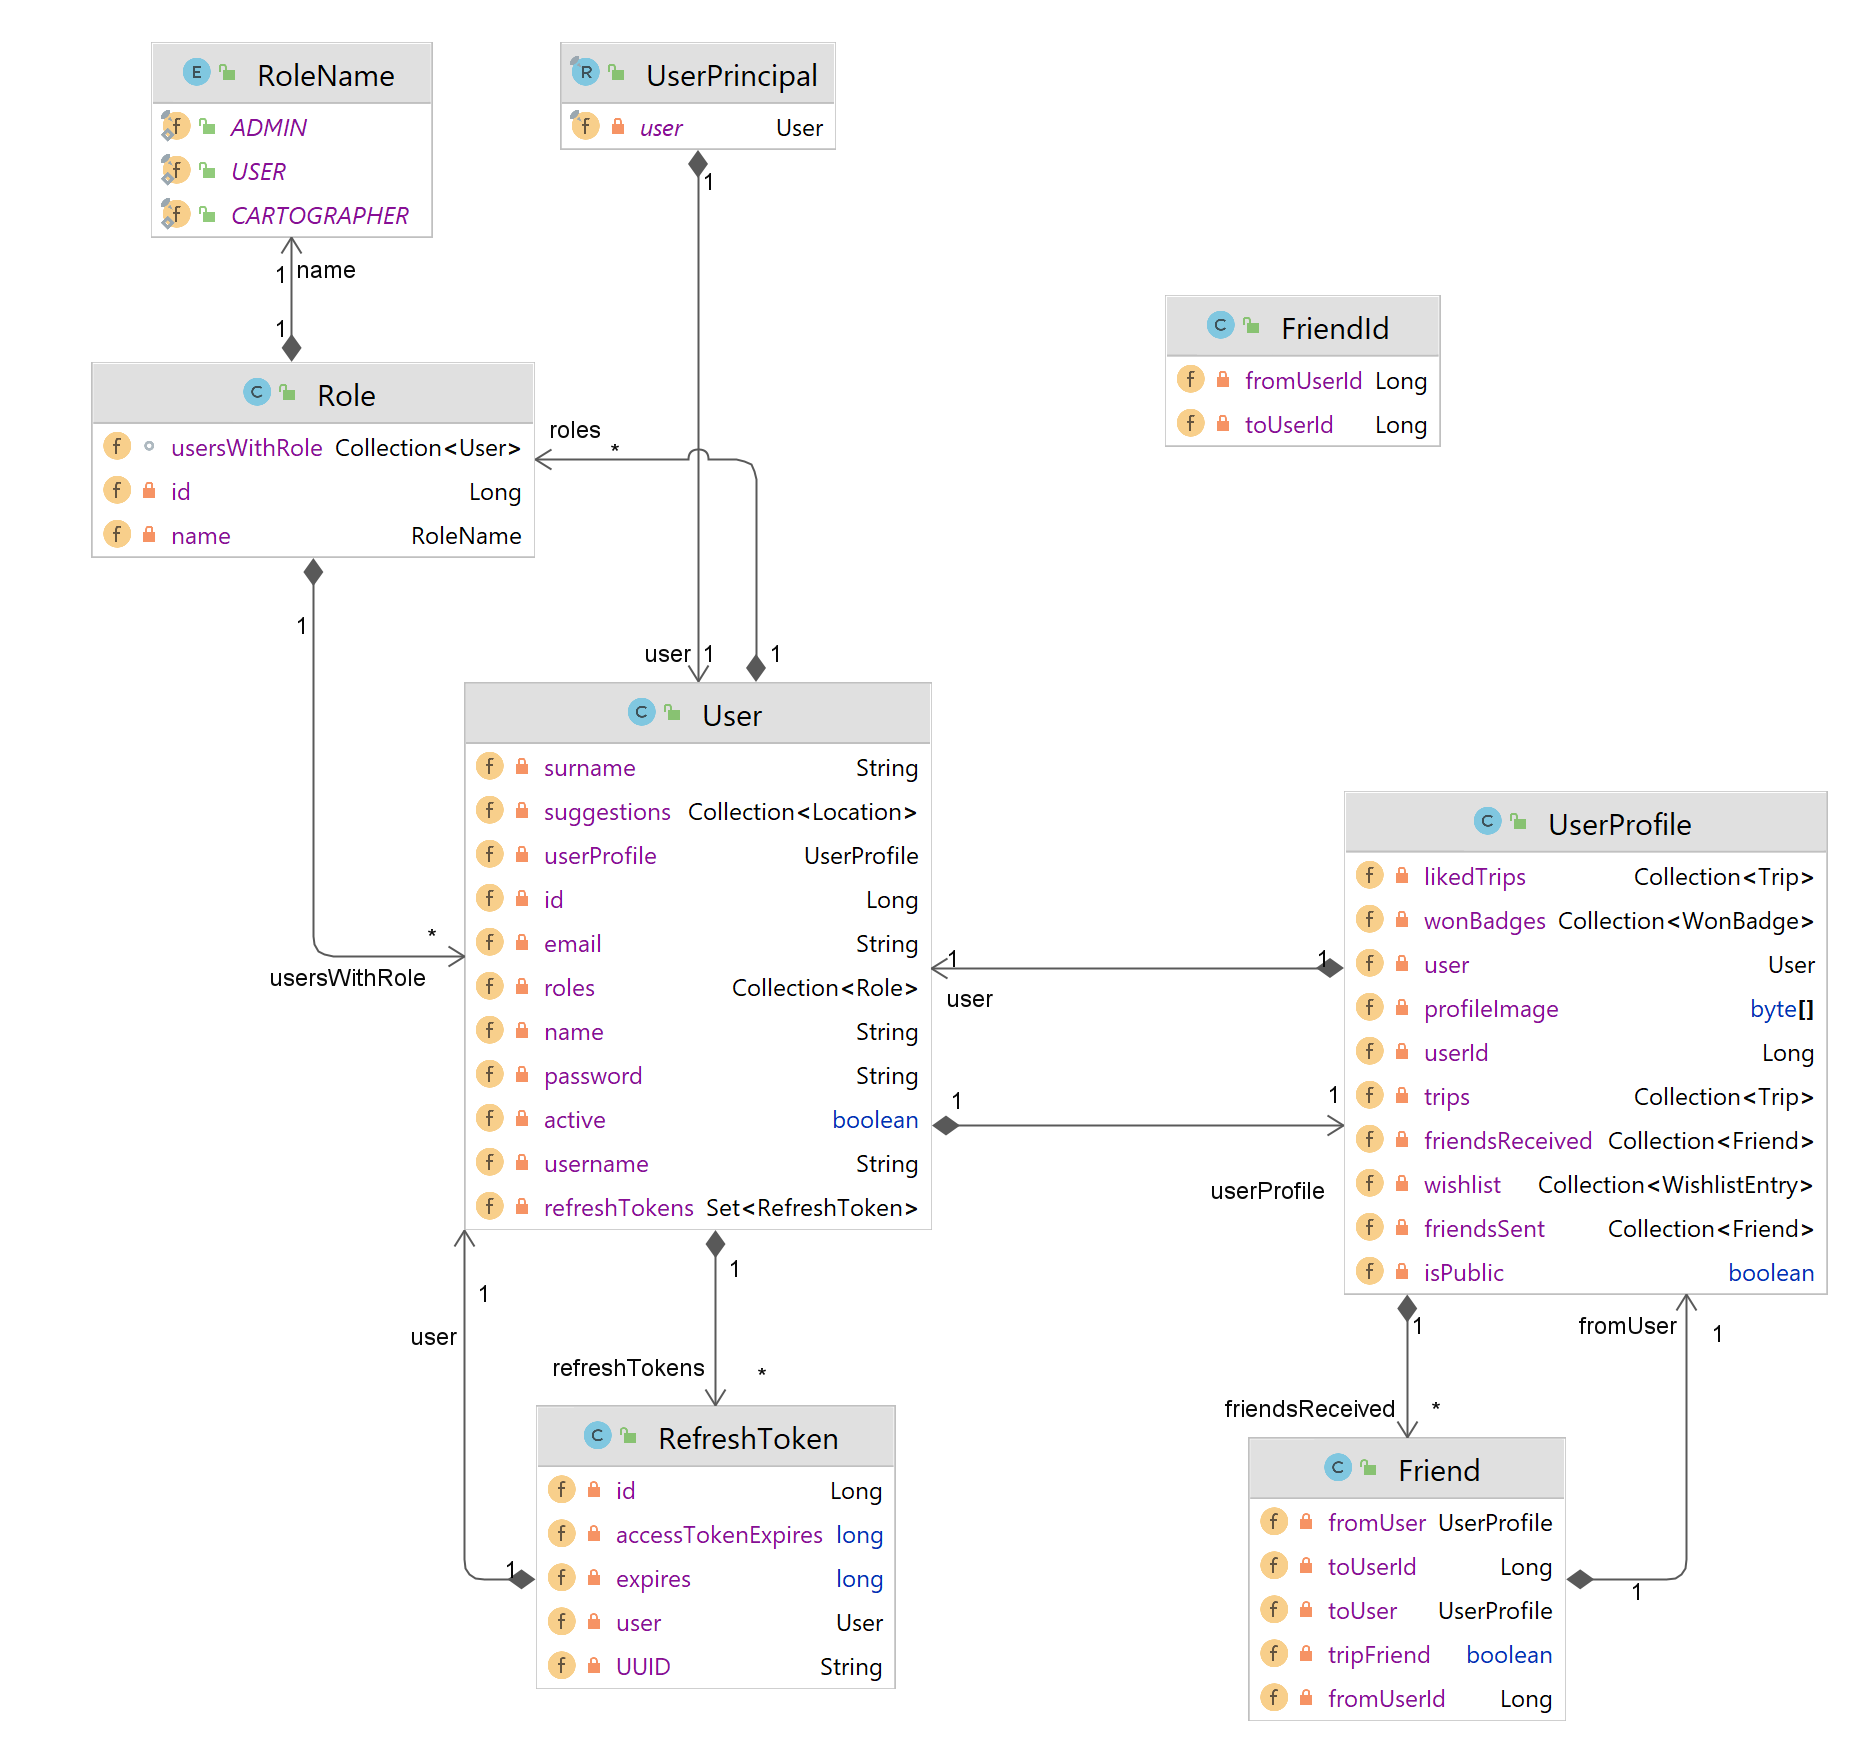
\includegraphics[scale=0.2]{slike/class/class_model_user.png}
        		\centering
        		\caption{Dijagram razreda - modeli korisnika}
        	\end{figure}
         
                \begin{figure}[H]
        			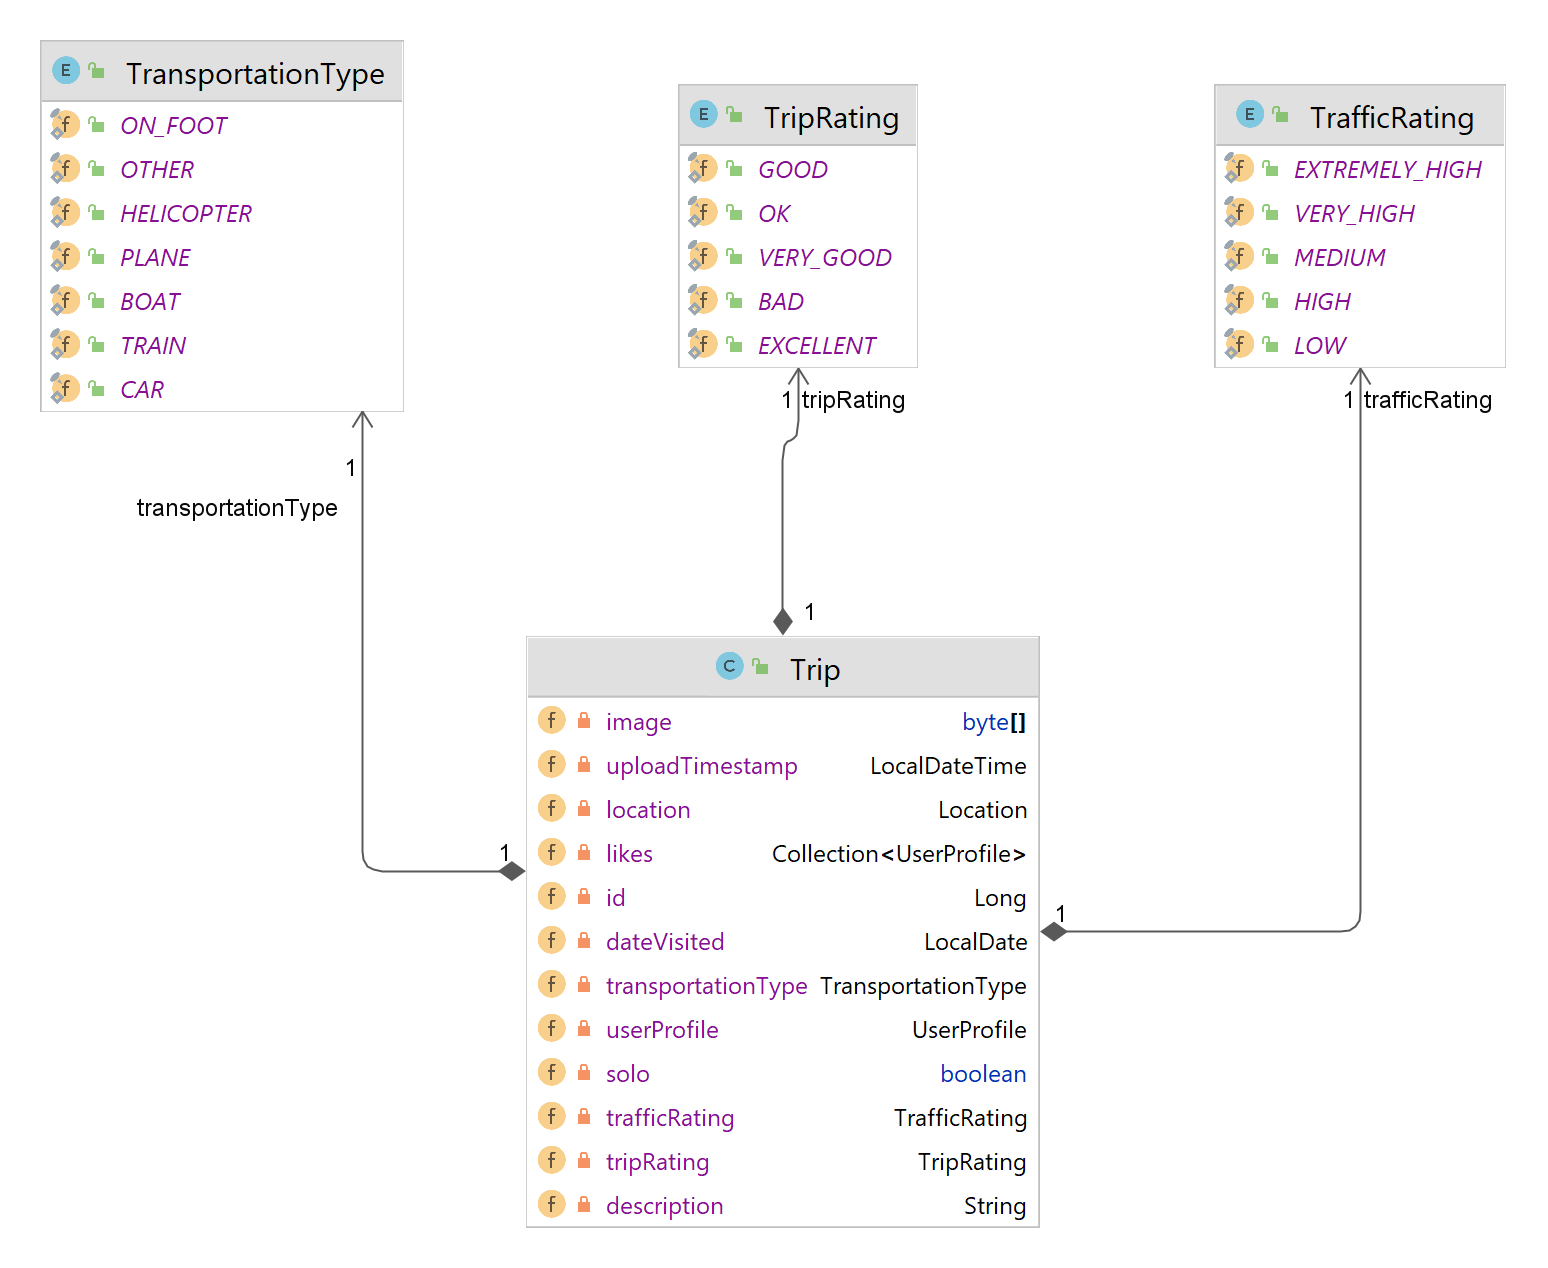
\includegraphics[scale=0.2]{slike/class/class_model_trip.png}
        		\centering
        		\caption{Dijagram razreda - modeli putovanja}
        	\end{figure}

                \begin{figure}[H]
        			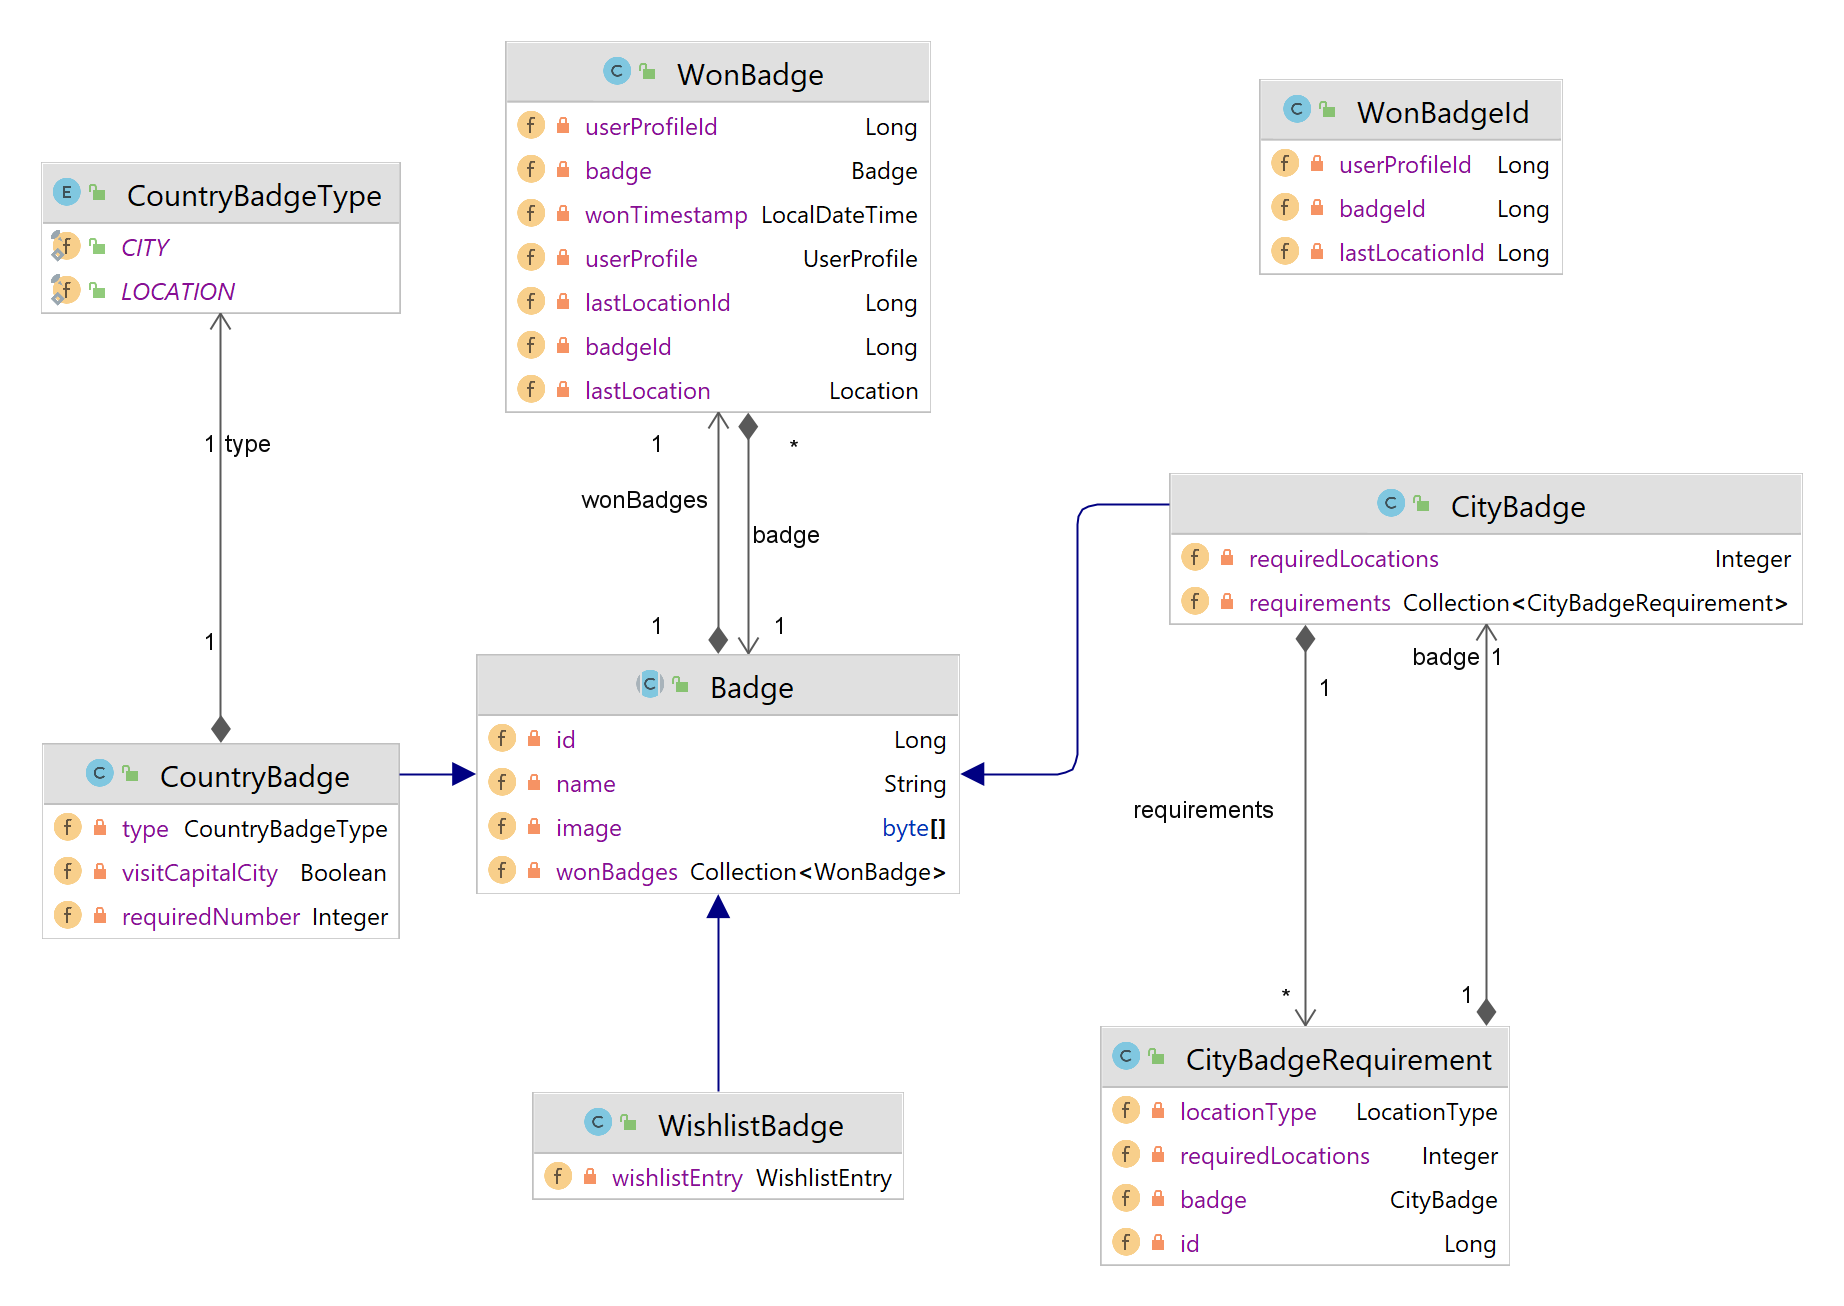
\includegraphics[scale=0.2]{slike/class/class_model_badge.png}
        		\centering
        		\caption{Dijagram razreda - modeli bedževa}
        	\end{figure}
         
                \begin{figure}[H]
        			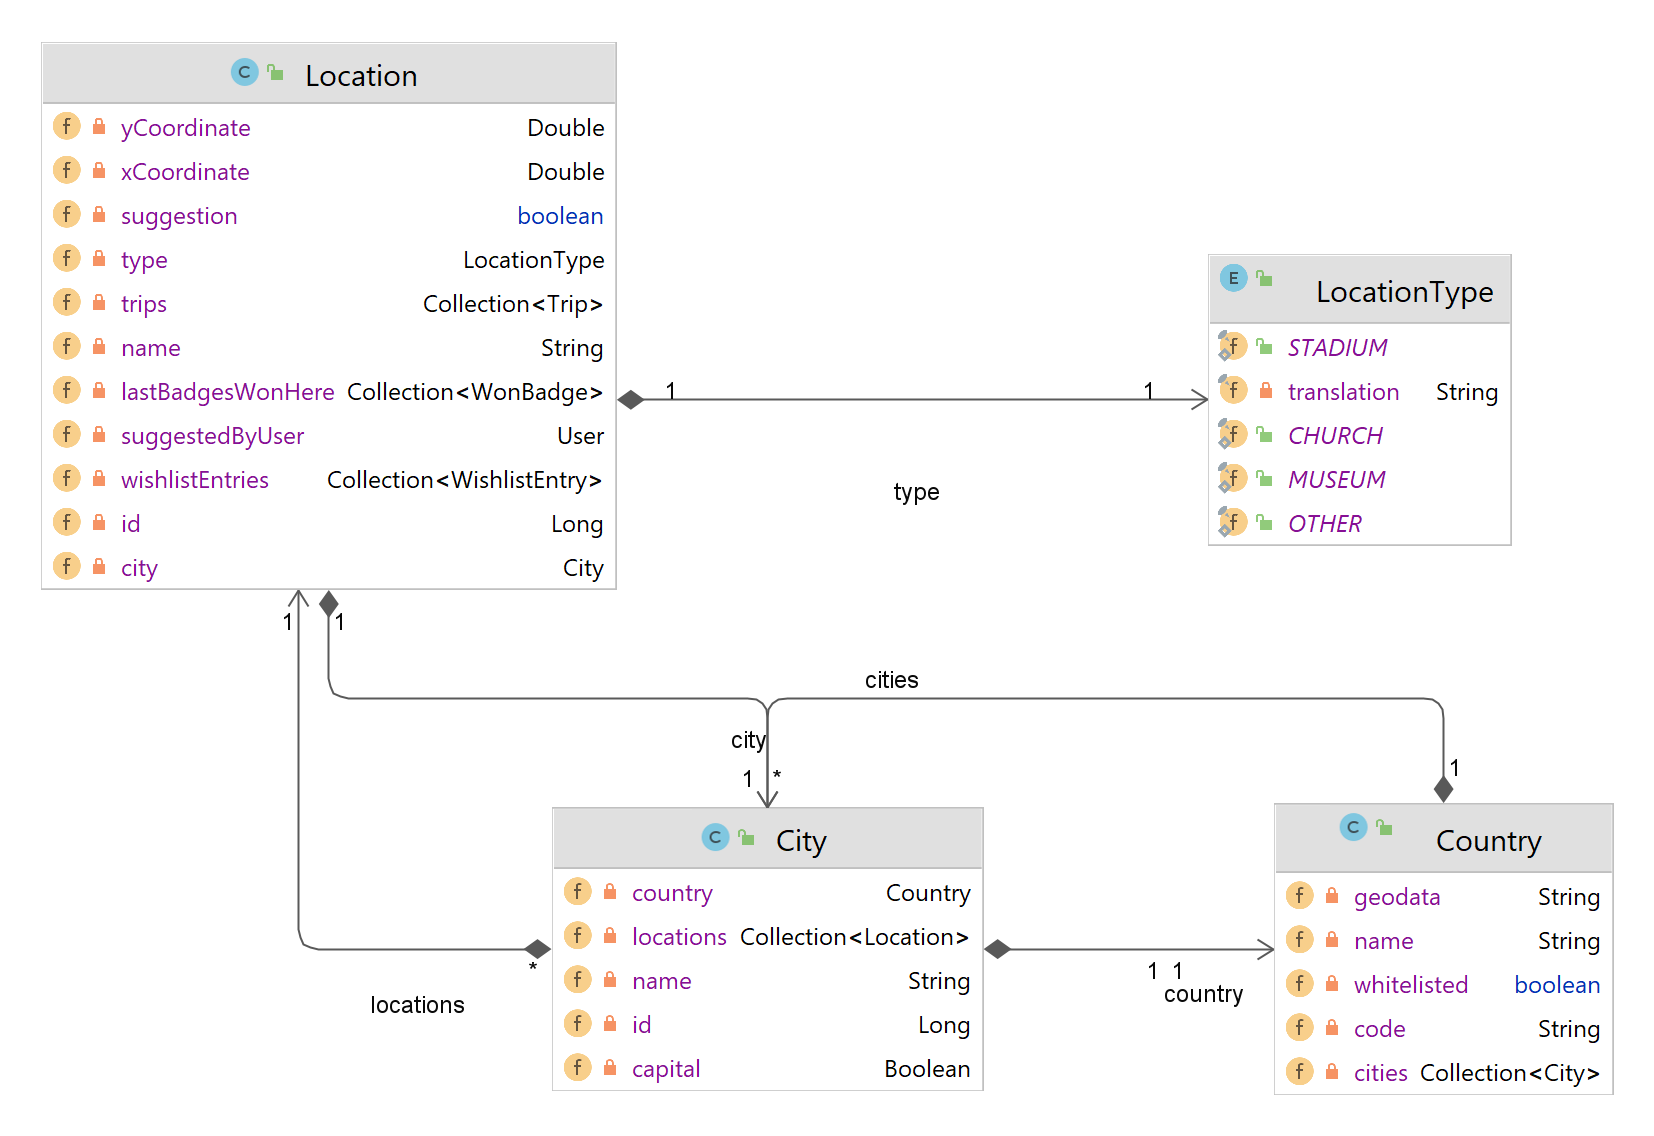
\includegraphics[scale=0.2]{slike/class/class_model_location.png}
        		\centering
        		\caption{Dijagram razreda - modeli lokacija}
        	\end{figure}
         
                \begin{figure}[H]
        			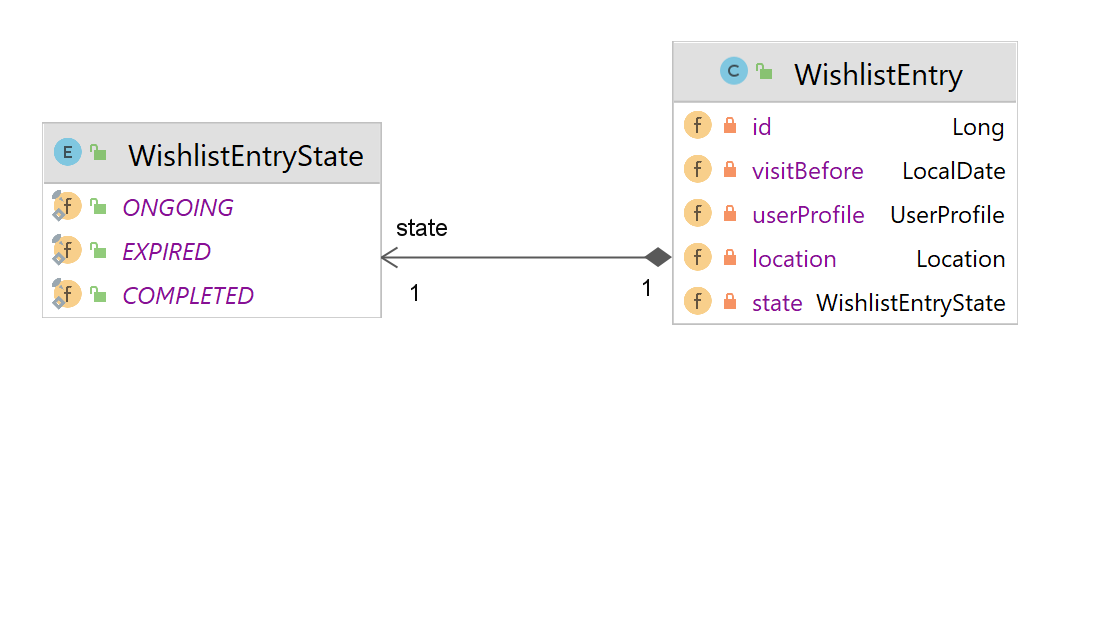
\includegraphics[scale=0.2]{slike/class/class_model_wishlist.png}
        		\centering
        		\caption{Dijagram razreda - modeli \textit{wishlist}-a}
        	\end{figure}

                 Na dijagramima razreda modela prikazani su razredi koji reprezentiraju sve relacije koje predstavljaju neki entitet u bazi podataka, sve vezne relacije koje sadrže dodatne atribute, kompozitne ključeve te enumeracije.
                \\
                \\
                Razredi modela za svako svoje svojstvo imaju metodu \textit{get} i \textit{set} te konstruktore.
                \eject


                \begin{figure}[H]
        			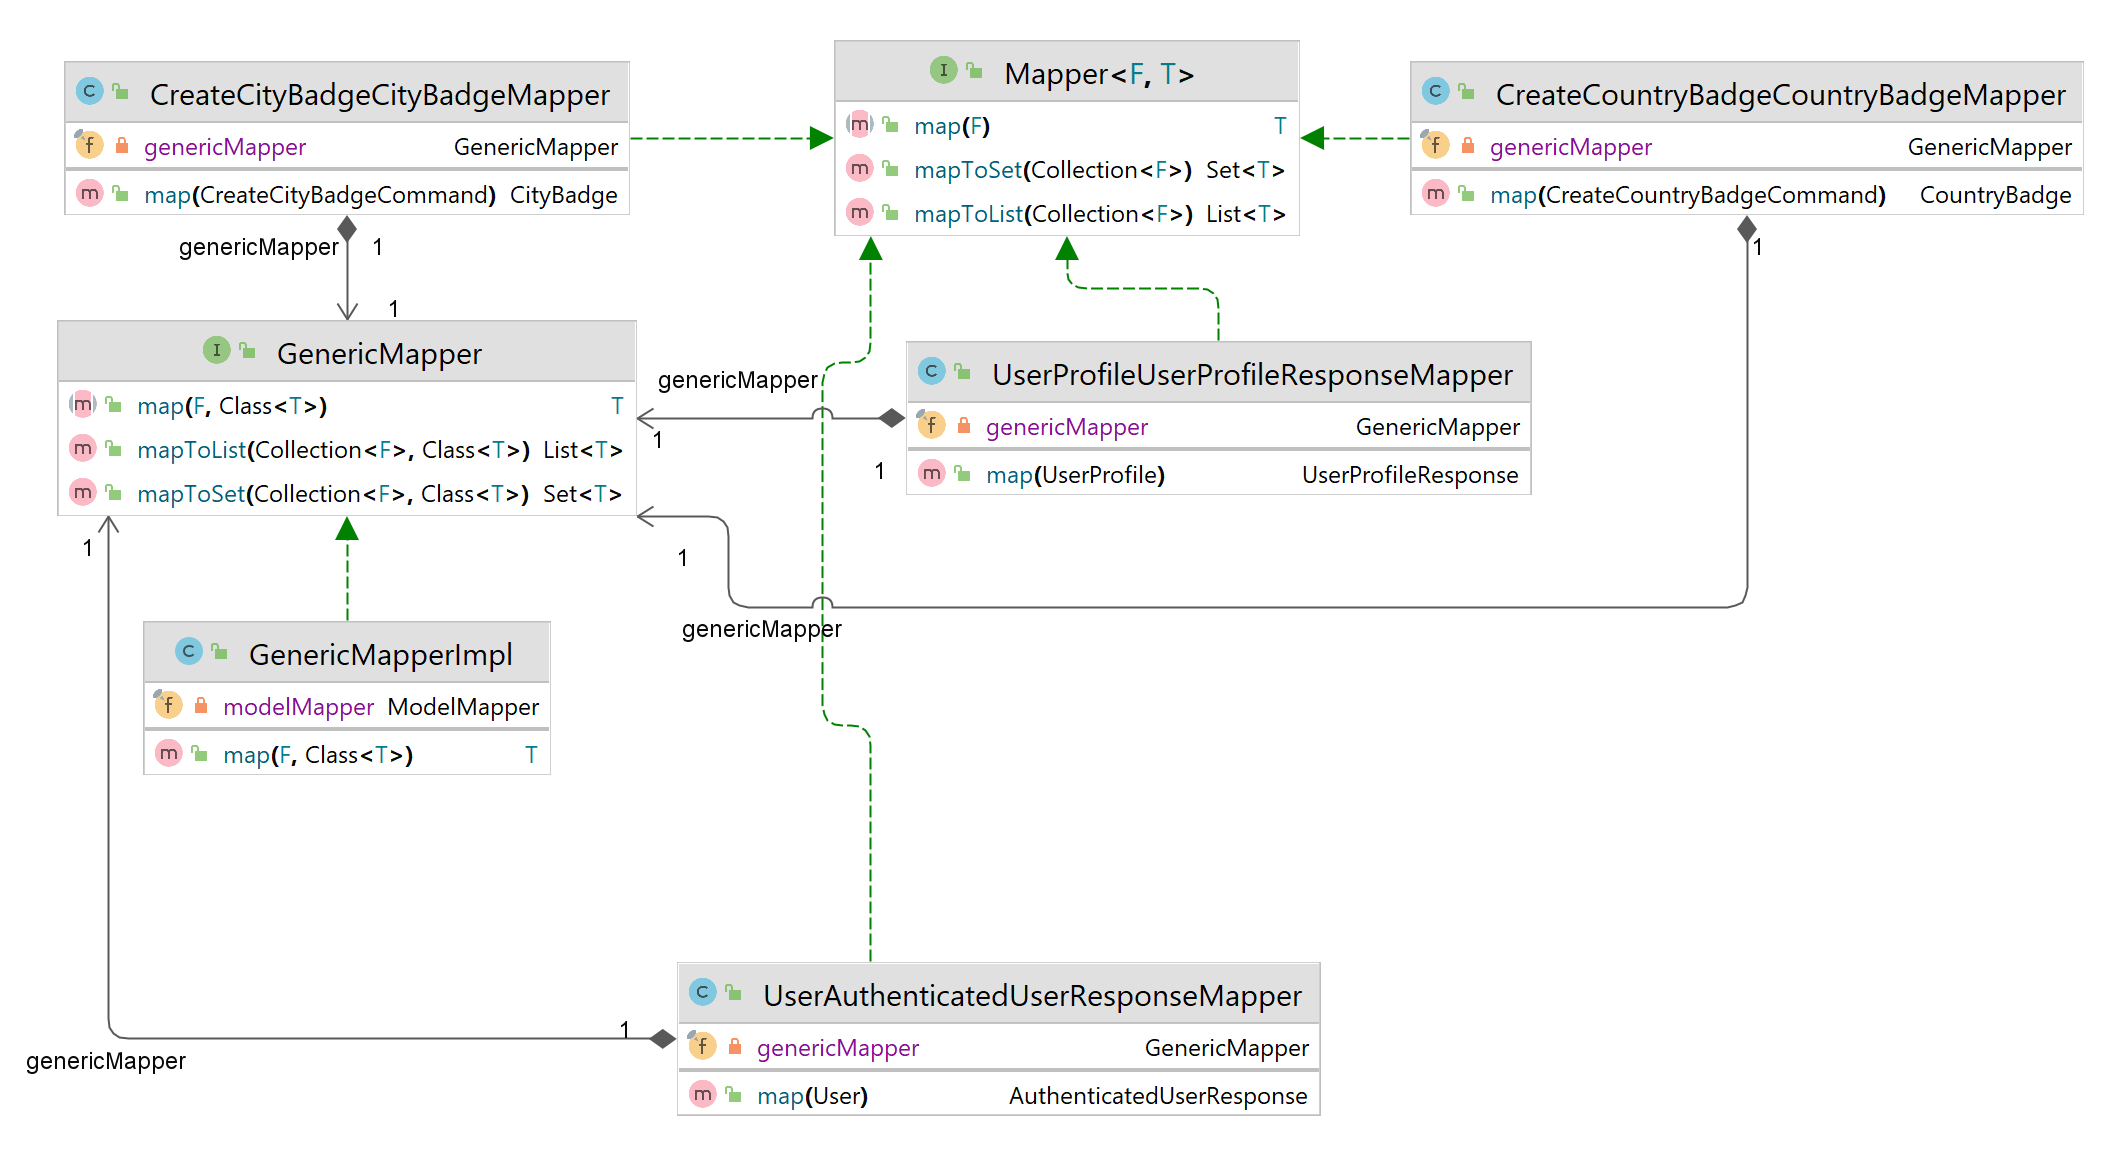
\includegraphics[scale=0.2]{slike/class/class_mapper.png}
        		\centering
        		\caption{Dijagram razreda - \textit{Mapper}}
        	\end{figure}
        

                \begin{figure}[H]
        			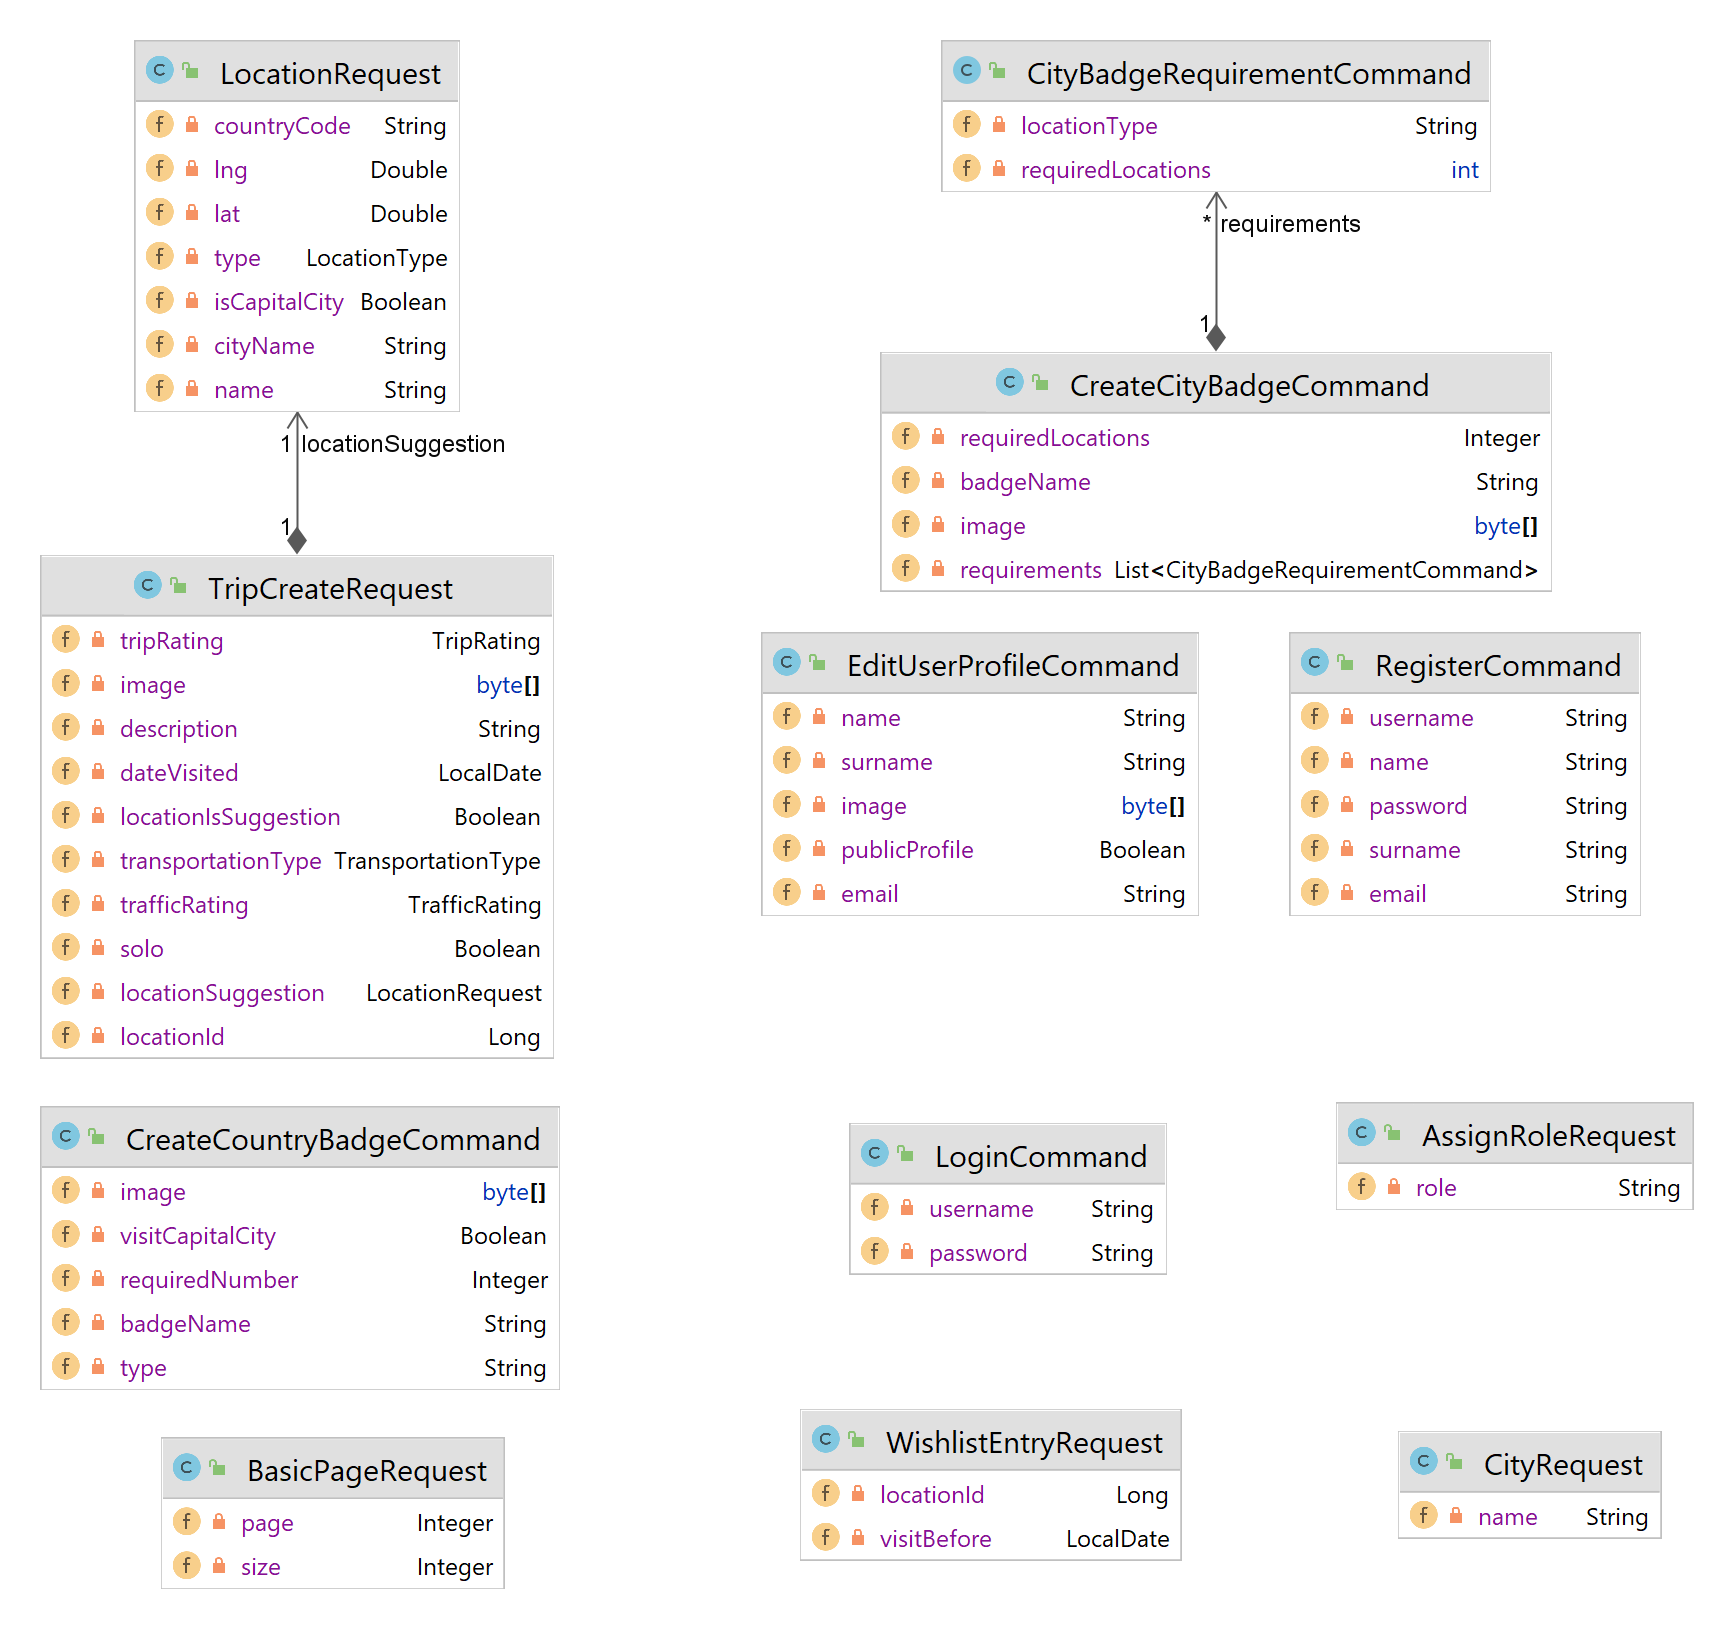
\includegraphics[scale=0.2]{slike/class/class_request.png}
        		\centering
        		\caption{Dijagram razreda - \textit{Request}}
        	\end{figure}

                \begin{figure}[H]
        			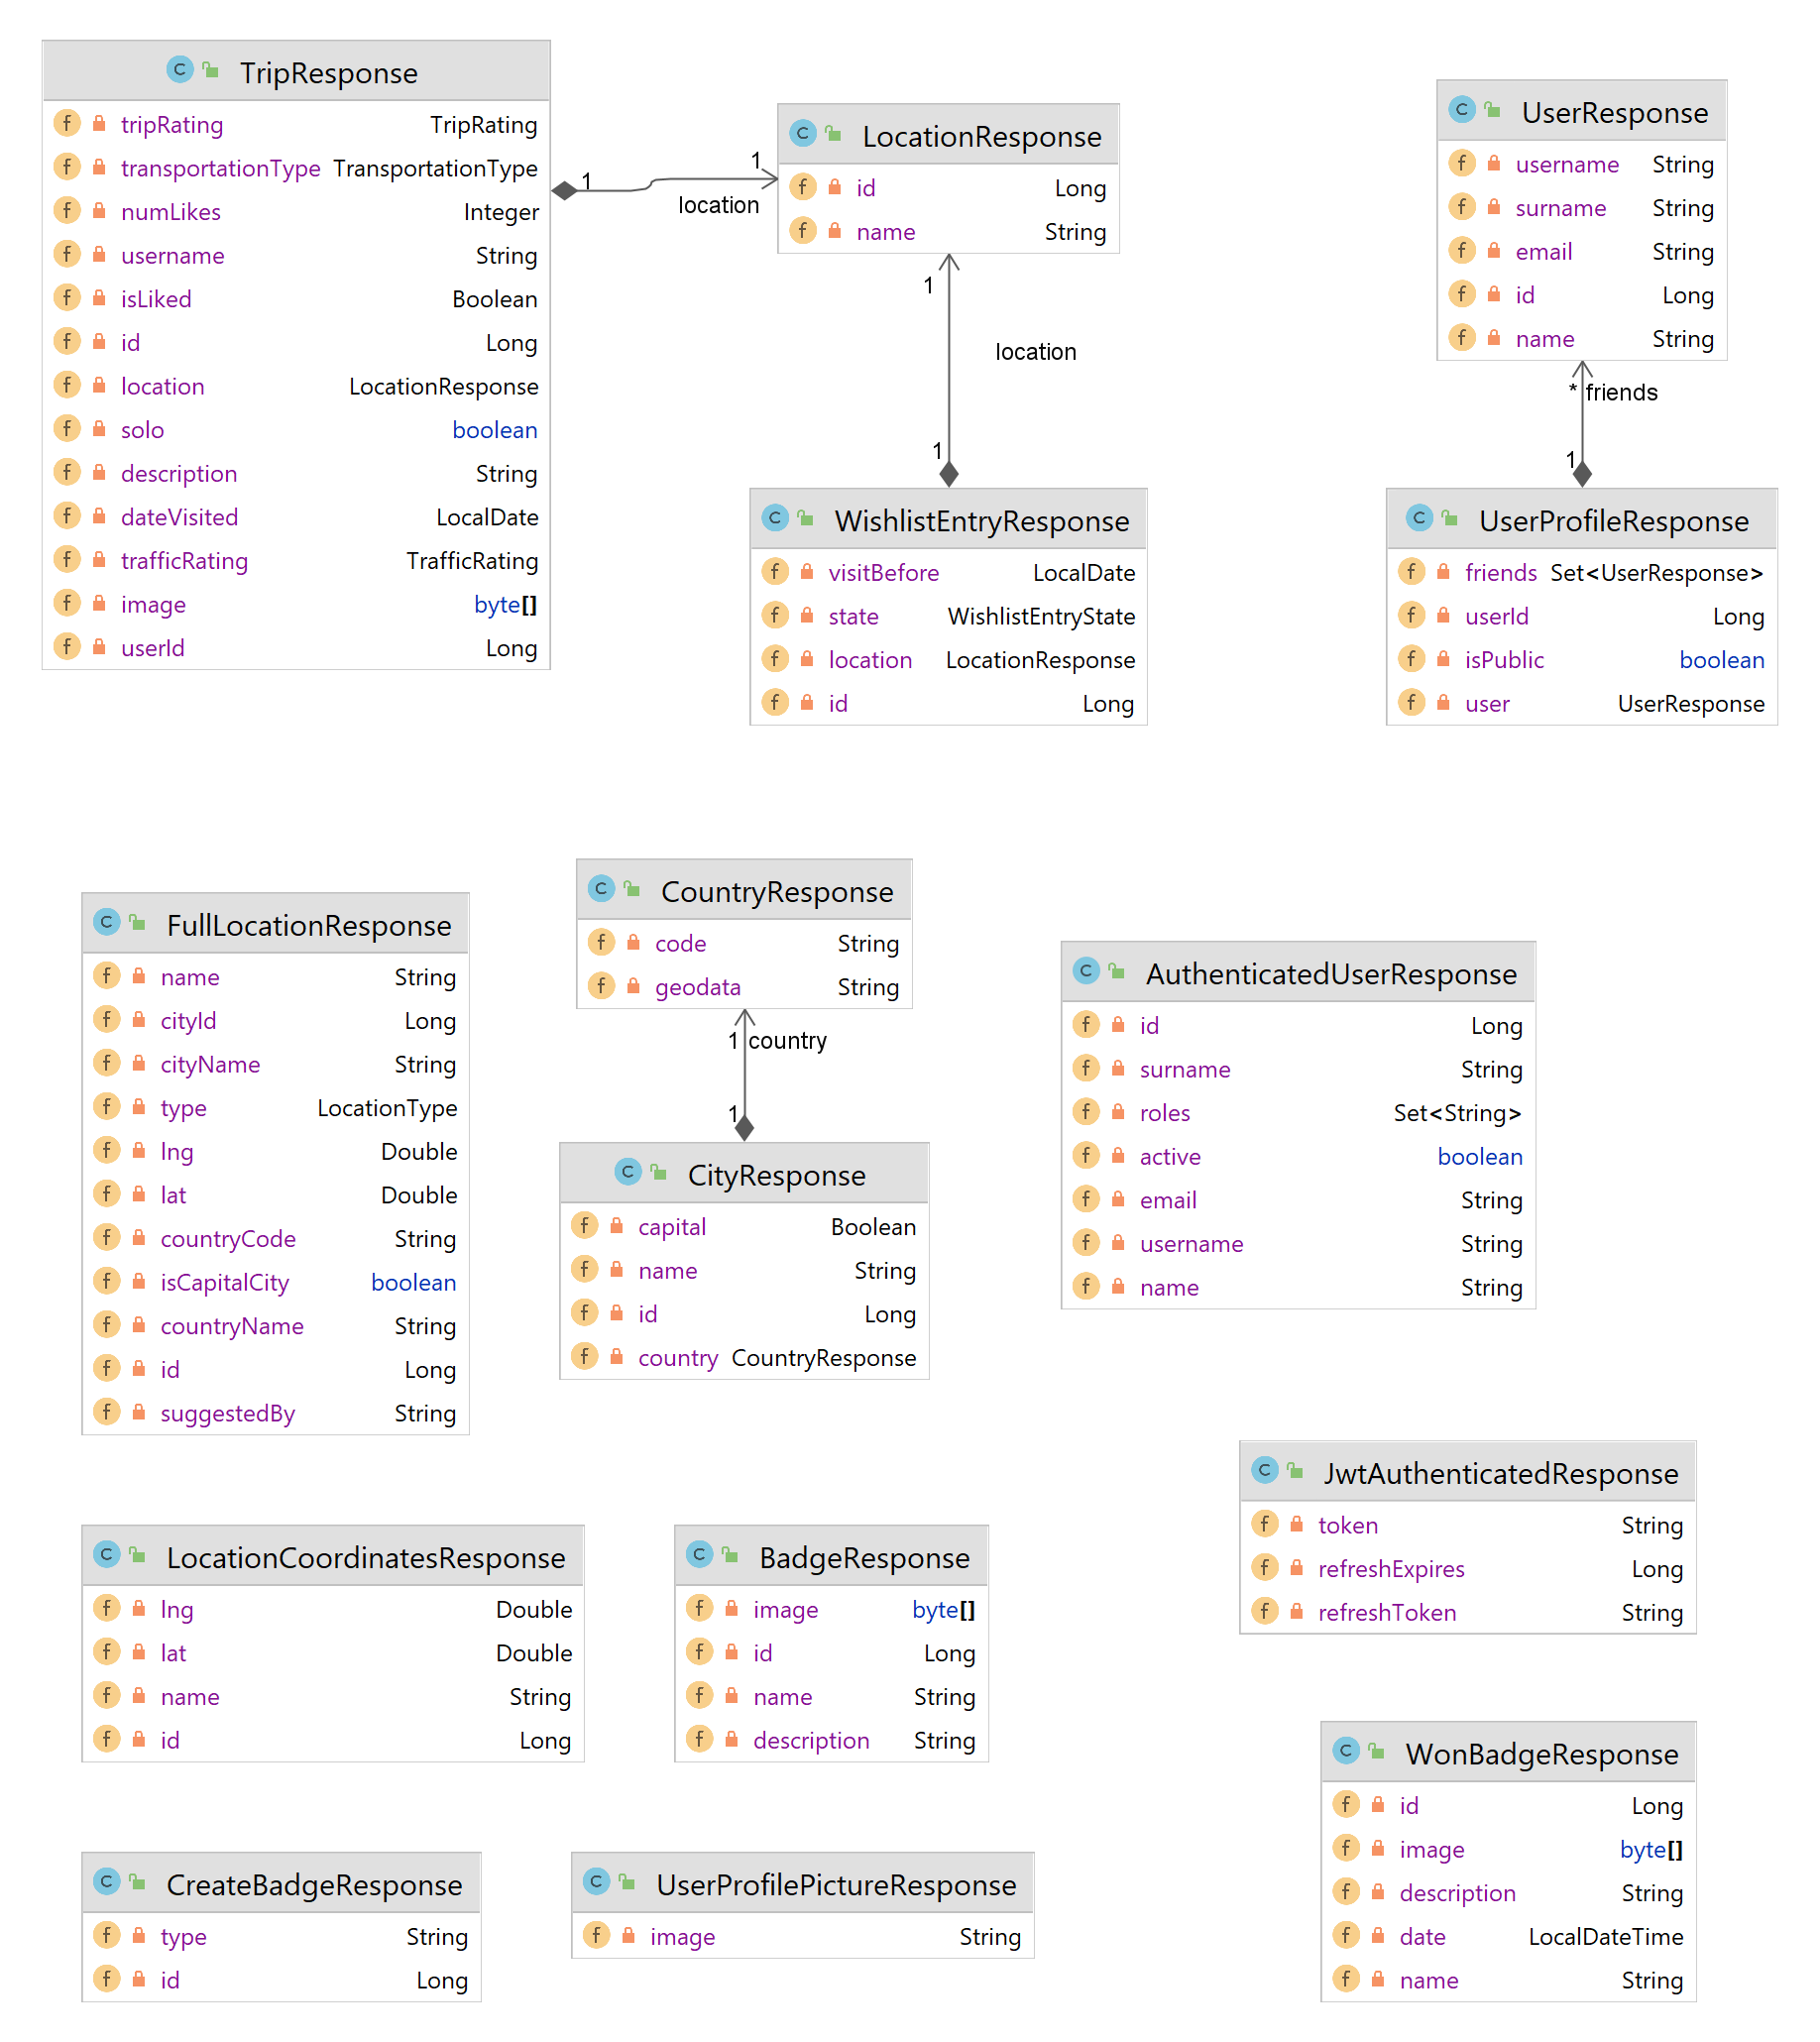
\includegraphics[scale=0.2]{slike/class/class_response.png}
        		\centering
        		\caption{Dijagram razreda - \textit{Response}}
        	\end{figure}
         \eject

                \begin{figure}[H]
        			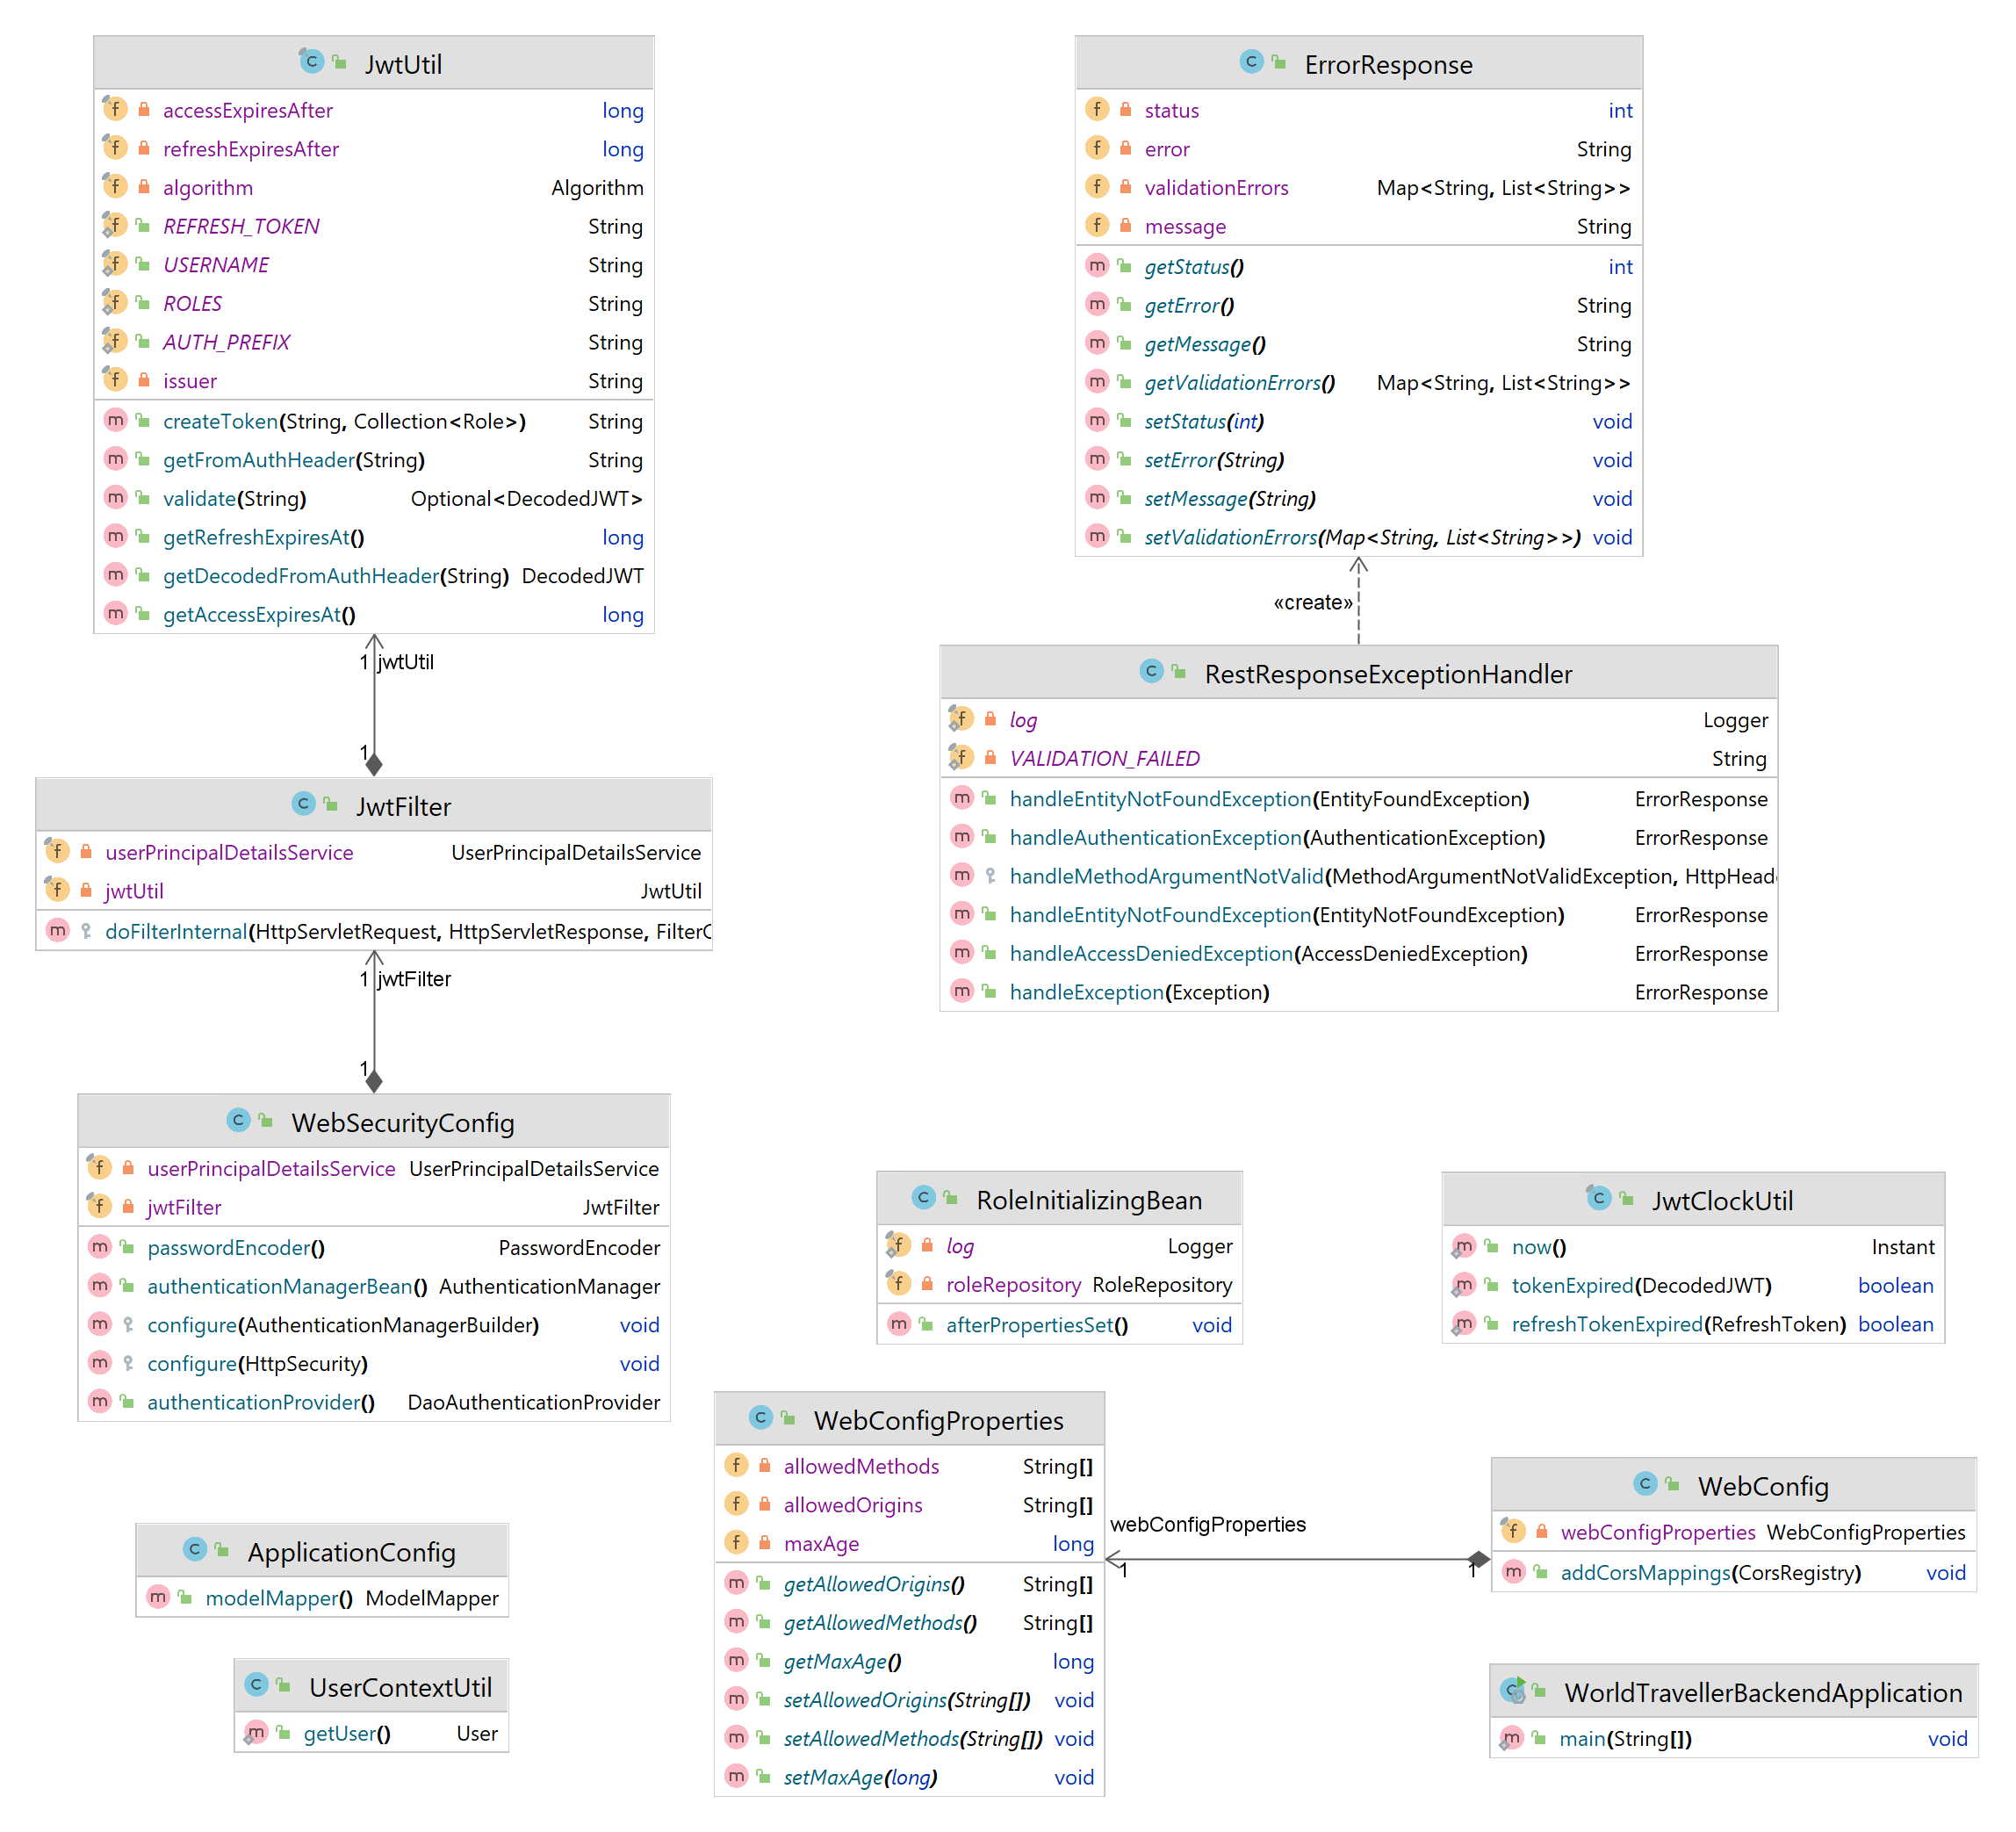
\includegraphics[scale=0.18]{slike/class/class_util_config.png}
        		\centering
        		\caption{Dijagram razreda - konfiguracijski i pomoćni razredi}
        	\end{figure}

			Na dijagramima prikazani su razredi koji se koriste za pokretanje Spring Boot-a, konfiguraciju autorizacije/autentifikacije i filtera, \textit{Exception} i \textit{util} razredi, generički \textit{Mapper} i njegove implementacije koje služi za pretvaranje razreda entiteta u \textit{DTO} (\textit{Request} i \textit{Response}) razred  te još neki konfiguracijski razredi.
            \eject
            
		\section{Dijagram stanja}


			%\textbf{\textit{dio 2. revizije}}\\

			%\textit{Potrebno je priložiti dijagram stanja i opisati ga. Dovoljan je jedan dijagram stanja koji prikazuje \textbf{značajan dio funkcionalnosti} sustava. Na primjer, stanja korisničkog sučelja i tijek korištenja neke ključne funkcionalnosti jesu značajan dio sustava, a registracija i prijava nisu. }
            
            Dijagram stanja prikazuje određenu funkcionalnost aplikacije pomoću automata. Dolje je prikazan dijagram stanja za regularnog korisnika, korisniku se prijavom prvo pokazuje naslovnica odakle može pristupit ostalim dijelovima aplikacije. S obzirom na način kako je implementirano sva "glavna" stanja su međusobno povezana odnosno čine potpuno povezanu mrežu, to su uz "Naslovnica", "Moji bedževi", "Moj profil", "Društvo", "Pretraživanje", "Lista želja" i "Moja putovanja". Iz svih stanja je moguće odjaviti se iz aplikacije. 
            \\
            Pregledavanjem vlastitog profila može se uređivati profil dodatnim klikom.
            Prilikom pretraživanja može se odabrati korisnik i pregledati profil navedenog korisnika.
            Iz stanja "Moja putovanja" moguće je dodati novo putovanje (objavu) ili ukloniti postojeću objavu.
            Na stranici "Lista želja" moguće je dodati novu želju na listu želja ili ukloniti postojeću želju sa liste želja.
            Iz stanja "Društvo" moguće je označiti objave prijatelja oznakom "Sviđa mi se".
            
            
                \begin{figure}[H]
        		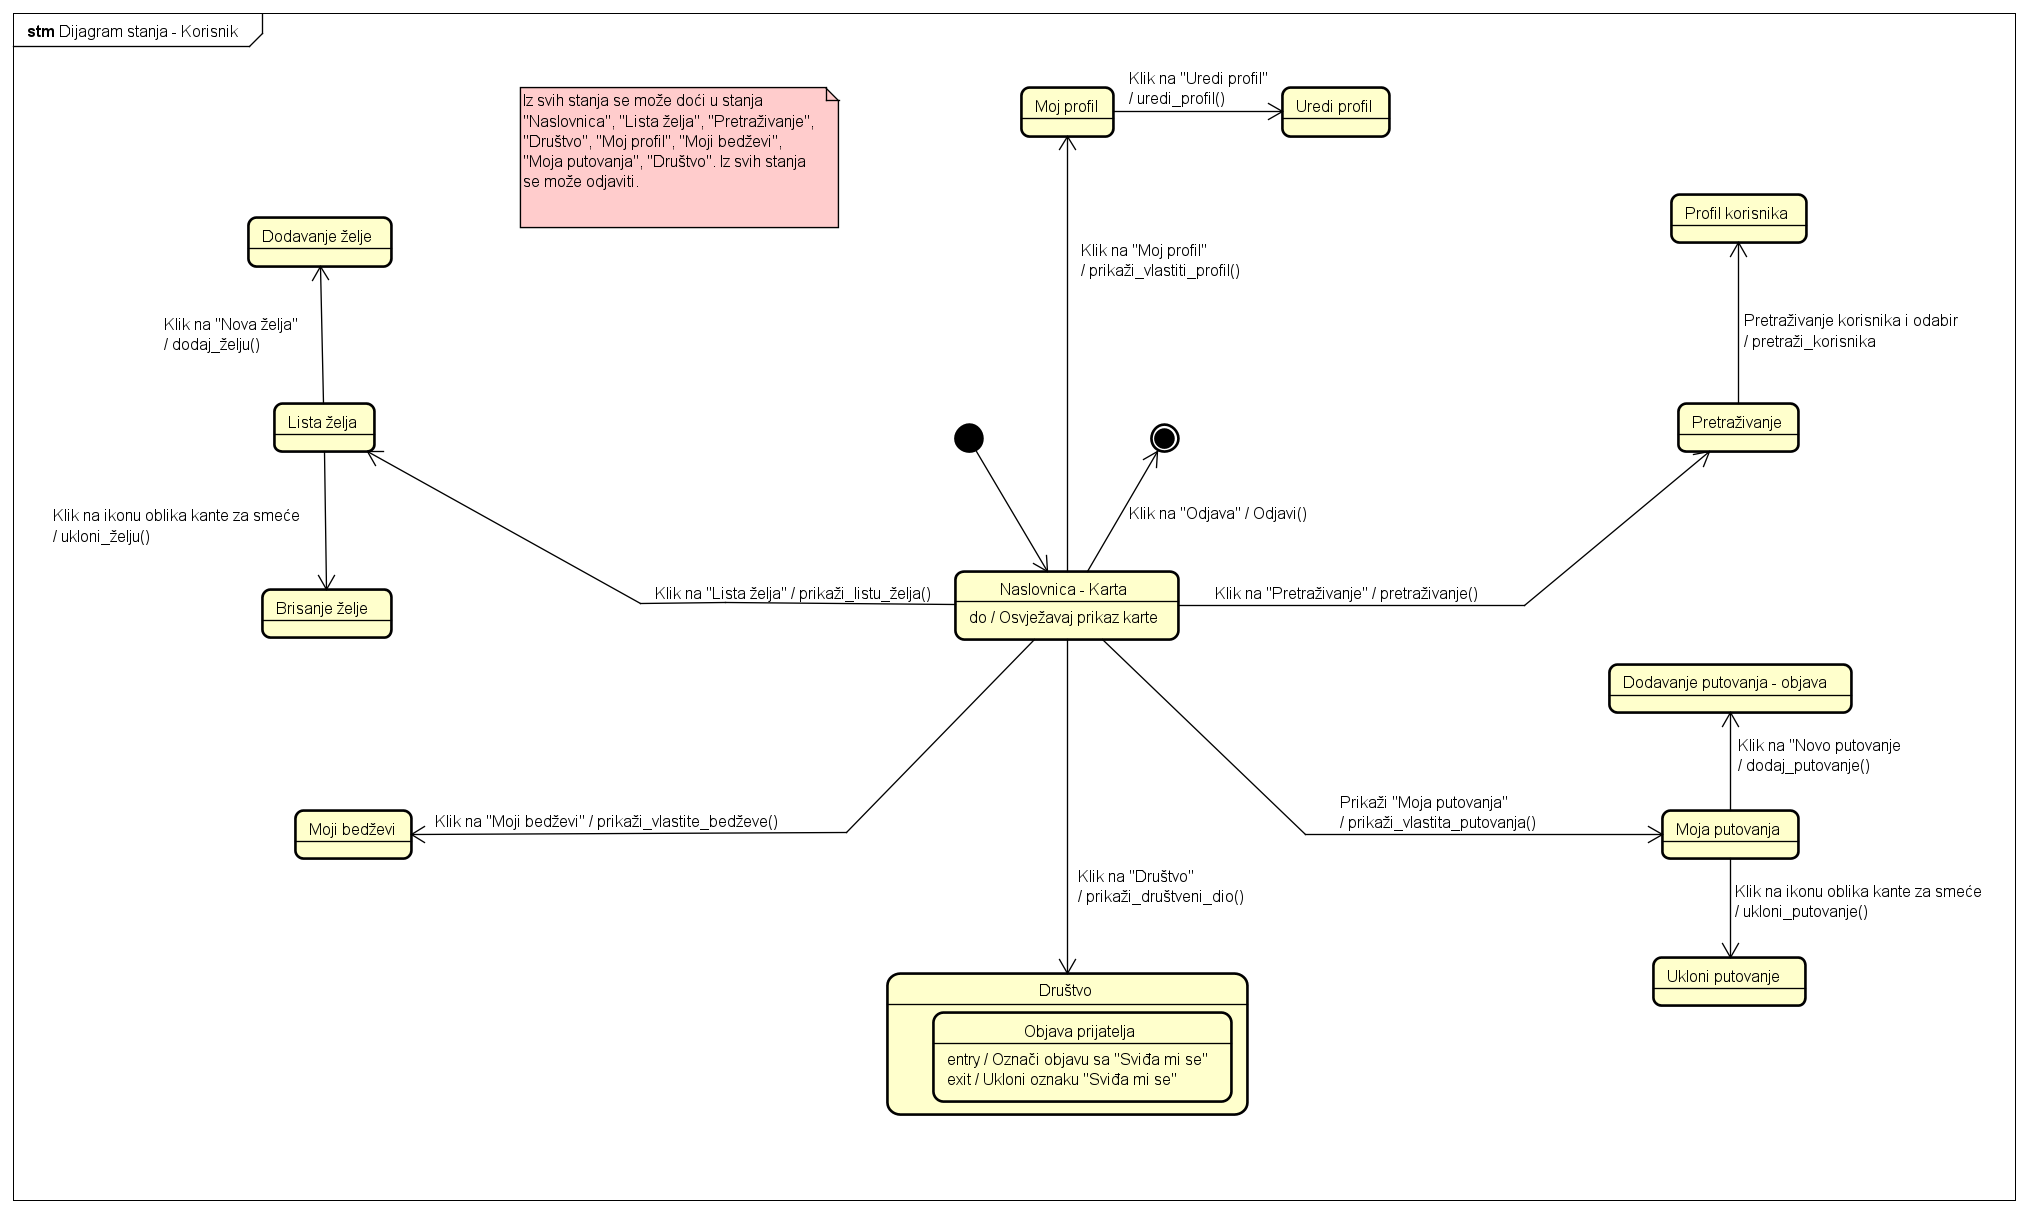
\includegraphics[scale=0.25]{slike/Dijagram stanja - Korisnik.png} %veličina slike u odnosu na originalnu datoteku i pozicija slike
        		  \centering
        		\caption{Dijagram stanja }

        	\end{figure}


			\eject

		\section{Dijagram aktivnosti}

			%\textbf{\textit{dio 2. revizije}}\\

			 %\textit{Potrebno je priložiti dijagram aktivnosti s pripadajućim opisom. Dijagram aktivnosti treba prikazivati značajan dio sustava.}

            Dijagram aktivnosti opisuje tok upravljanja određenog dijela aplikacije. Na dijagramu aktivonsti ispod prikazan je proces objavljivanja putovanja.
            \\
            Korisnik odabire opciju "Nova objava" zatim mu se prikazuje forma za izradu nove objave (putovanja) te mu se prikazuje karta za označavanje mjesta. Nakon provjere označene lokacije i uvjeta bedževa sprema se putovanje (po potrebi lokacija i osvojen bedž) te se korisniku prikazuje stranica s novim putovanjem dodanim.

                \begin{figure}[H]
        		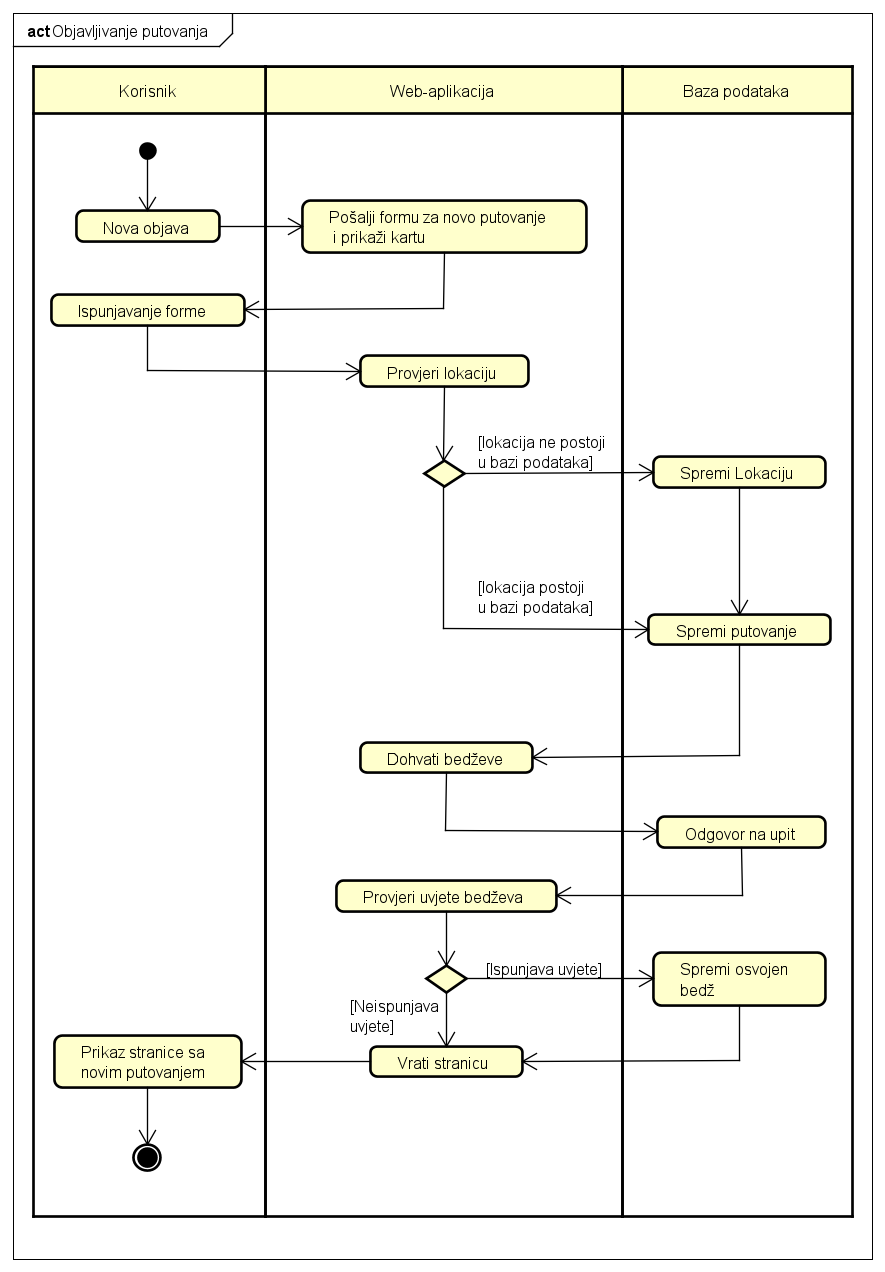
\includegraphics[scale=0.45]{slike/Dijagram aktivnosti - Objavljivanje putovanja.png} %veličina slike u odnosu na originalnu datoteku i pozicija slike
        		  \centering
        		\caption{Dijagram aktivnosti }

        	\end{figure}
         
			\eject
		\section{Dijagram komponenti}

			%\textbf{\textit{dio 2. revizije}}\\

			 %\textit{Potrebno je priložiti dijagram komponenti s pripadajućim opisom. Dijagram komponenti treba prikazivati strukturu cijele aplikacije.}
            

            Dijagram komponenti prikazuje organizaciju i internu strukturu aplikacije. Na dijagramu komponenti ispod prikazana je struktura aplikacije Svjetski putnik.
            Sustavu se pristupa preko dva sučelja, jednim koji komunicira sa dijelom \textit{frontenda} i jednim koji komunicira sa dijelom \textit{backenda} (i baze podataka). Preko sučelja za dohvat CSS, JS i TS datoteka poslužuju se datoteke koje pripadaju \textit{frontend} dijelu, a preko sučelja za dohvat JSON datoteka poslužuju se datoteke koje pripadaju \textit{backend} dijelu.
            \\
            Sve JS/TS datoteke ovise o React \textit{library-u} iz koje dohvaćaju potrebne komponente. REST API poslužuje podatke koji pripadaju \textit{backend} dijelu aplikacije, odnosno pruža JSON podatke. JPA je zadužen za dohvaćanje tablica iz baze podataka.

                \begin{figure}[H]
        		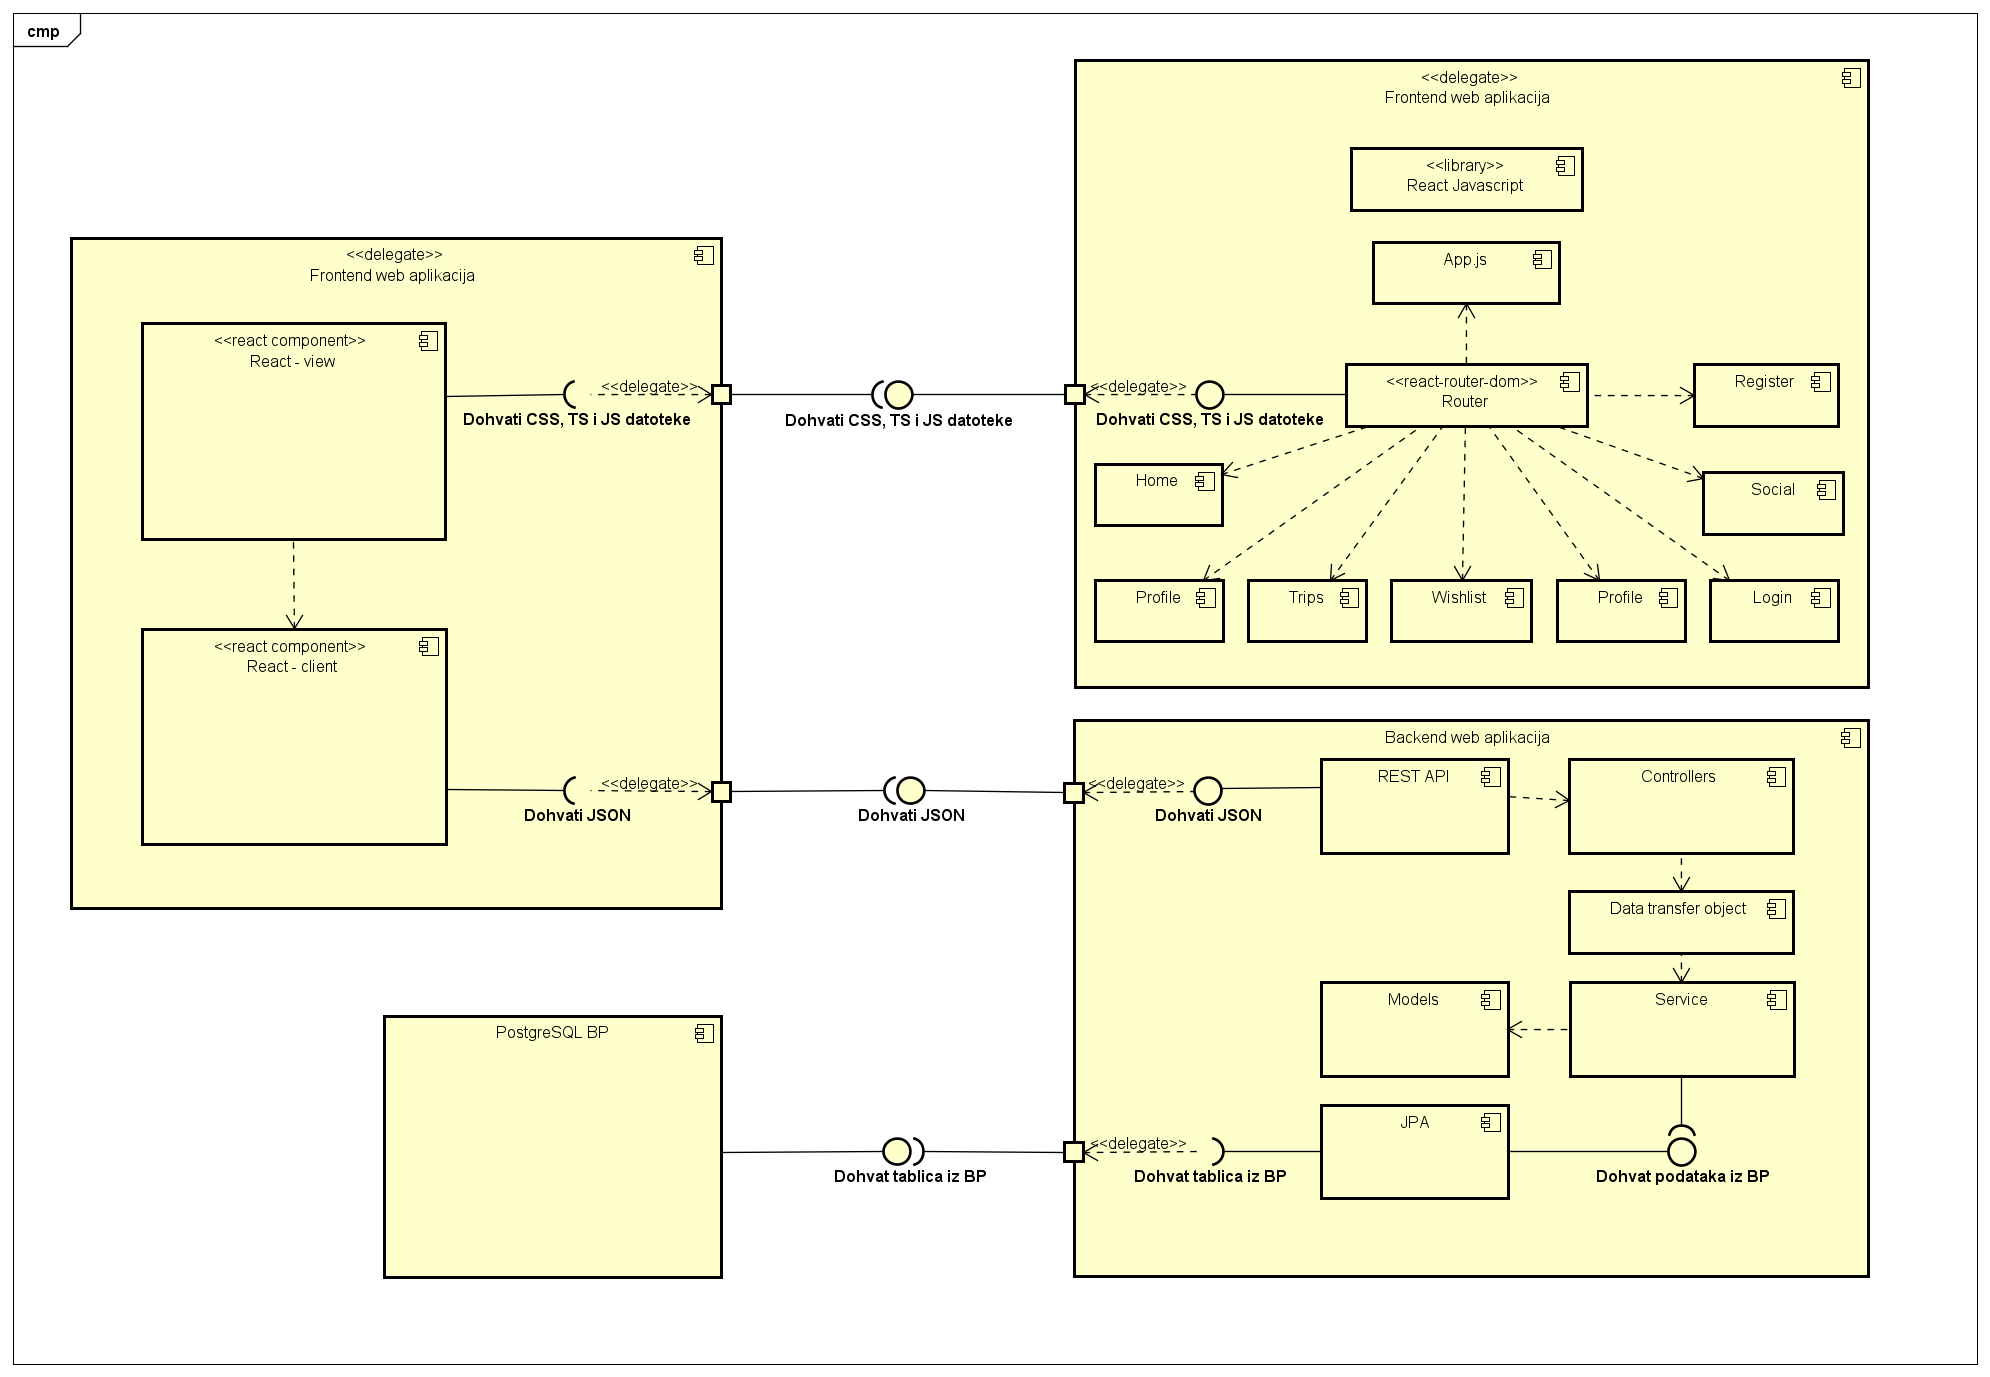
\includegraphics[scale=0.3]{slike/Dijagram komponenti.png} %veličina slike u odnosu na originalnu datoteku i pozicija slike
        		  \centering
        		\caption{Dijagram komponenti}

        	\end{figure}
         \eject
	
\chapter{Implementacija i korisničko sučelje}
		
		
		\section{Korištene tehnologije i alati}
		
		%\textbf{\textit{dio 2. revizije}}
			
			 %\textit{Detaljno navesti sve tehnologije i alate koji su primijenjeni pri izradi dokumentacije i aplikacije. Ukratko ih opisati, te navesti njihovo značenje i mjesto primjene. Za svaki navedeni alat i tehnologiju je potrebno \textbf{navesti internet poveznicu} gdje se mogu preuzeti ili više saznati o njima}.
            Komunikacija u timu ostvarena je korištenjem aplikacija \underline{\href{https://web.whatsapp.com/}{WhatsApp}} i \underline{\href{https://discord.com/}{Discord}}, za izradu UML dijagrama korišten je alat \underline{\href{https://astah.net/}{Astah UML}}, a za organizaciju i upravljanje izvornim kodom korišten je sustav \underline{\href{https://git-scm.com/}{Git}}. Kao udaljeni repozitorij projekta korištena je web platforma \underline{\href{https://gitlab.com/}{GitLab}}. Za oblikovanje dokumentacije korišten je alat \underline{\href{www.overleaf.com}{Overleaf}} koji omogućuje prevođenje jezika LaTeX bez posebnih alata.
            \\
            \\
            Razvojno okruženje korišteno za izradu \textit{backend} dijela aplikacije je \underline{\href{https://www.jetbrains.com/idea/}{Jetbrains IntelliJ IDEA}}, IntelliJ olakšava razvoj aplikacija i web-stranica u programskom jeziku Java (uz Spring boot). Za izradu \textit{frontend} dijela aplikacije korišten je \underline{\href{https://code.visualstudio.com/}{Visual Studio Code}} razvojno okruženje s obzirom da treba koristiti više tehnologija odjednom: React, Javascript, Typescript, CSS i slično.
            Za bazu podataka korišten je PostgreSQL a za upravljanje bazom podataka korišten je alat \underline{\href{https://dbeaver.io/}{DBeaver}}.
			
			
			\eject 
		
	
		\section{Ispitivanje programskog rješenja}
			
			\subsection{Ispitivanje komponenti}
			Provedeno je ispitivanje komponenti koristeći okvire za jedinično ispitivanje \underline{\href{https://junit.org/junit5/}{JUnit}} i \underline{\href{https://site.mockito.org/}{Mockito}}. 
           \\
           \\
           Ispituju se metode razreda \textit{BadgeService}, \textit{LocationService} te \textit{TripService}. Ispitni slučajevi sadrže ispitivanje regularnog ponašanja te bacanja iznimki. 
           \\
           \\
           Prije pokretanja ispitnih slučajeva inicijaliziraju se objekti korišteni u ispitnim slučajevima u \textit{initData()} metodi koja je anotirana s \textit{@BeforeEach} (zbog njene duljine, navedena metoda nije prikazana na slikama).
			
        \begin{figure}[H]
            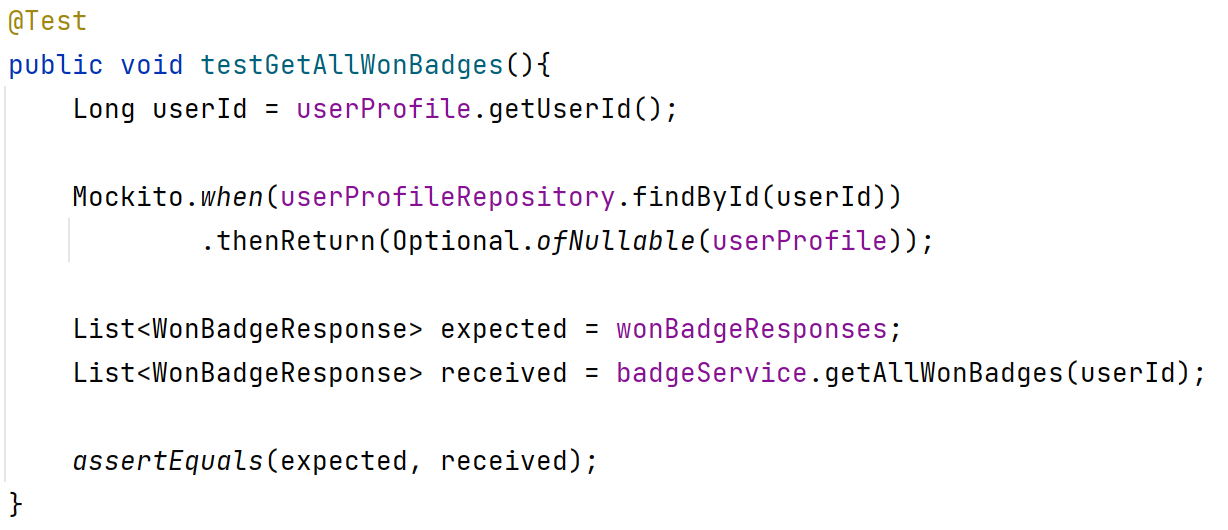
\includegraphics[scale=0.9]{slike/unit_test_badge_get_all.png} 
              \centering
            \caption{Ispitni slučaj - razred \textit{BadgeService} - metoda \textit{getAllWonBadges}}
        \end{figure}

         \begin{figure}[H]
            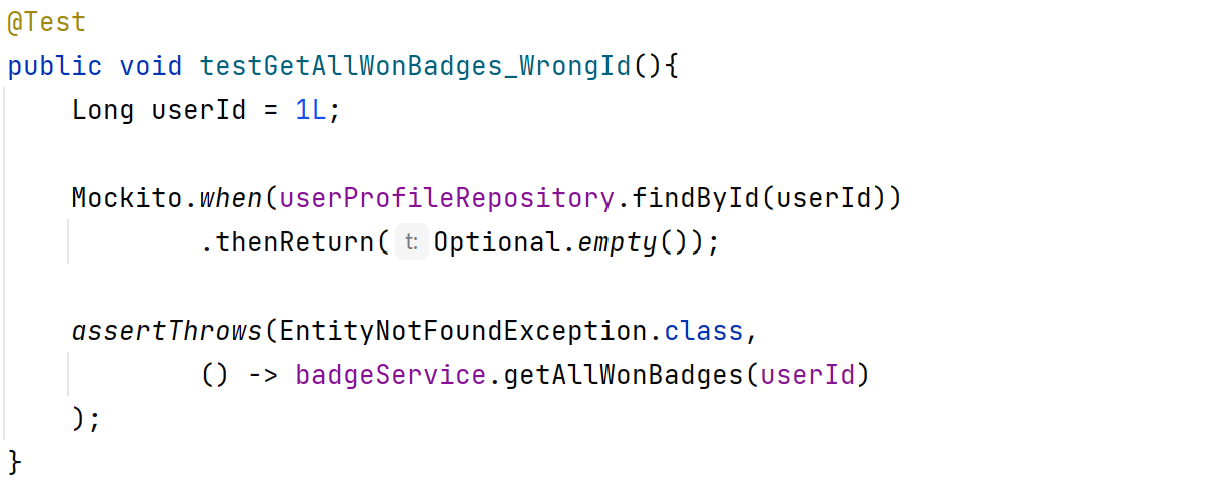
\includegraphics[scale=0.9]{slike/unit_test_location_wrong_id.png} 
              \centering
            \caption{Ispitni slučaj - razred \textit{BadgeService} - metoda \textit{getAllWonBadges} - bacanje iznimke}
        \end{figure}

        \begin{figure}[H]
            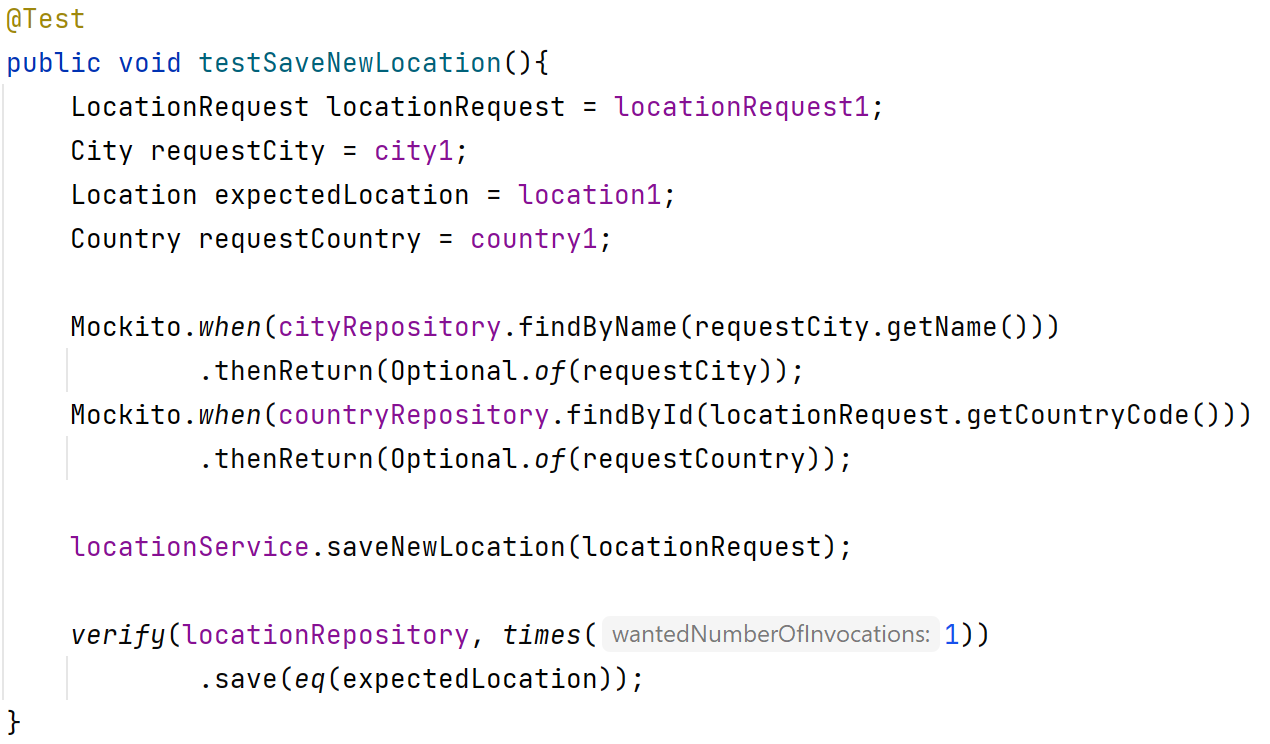
\includegraphics[scale=0.9]{slike/unit_test_location_save.png} 
              \centering
            \caption{Ispitni slučaj - razred \textit{LocationService} - metoda \textit{saveNewLocation}}
        \end{figure}

        \begin{figure}[H]
            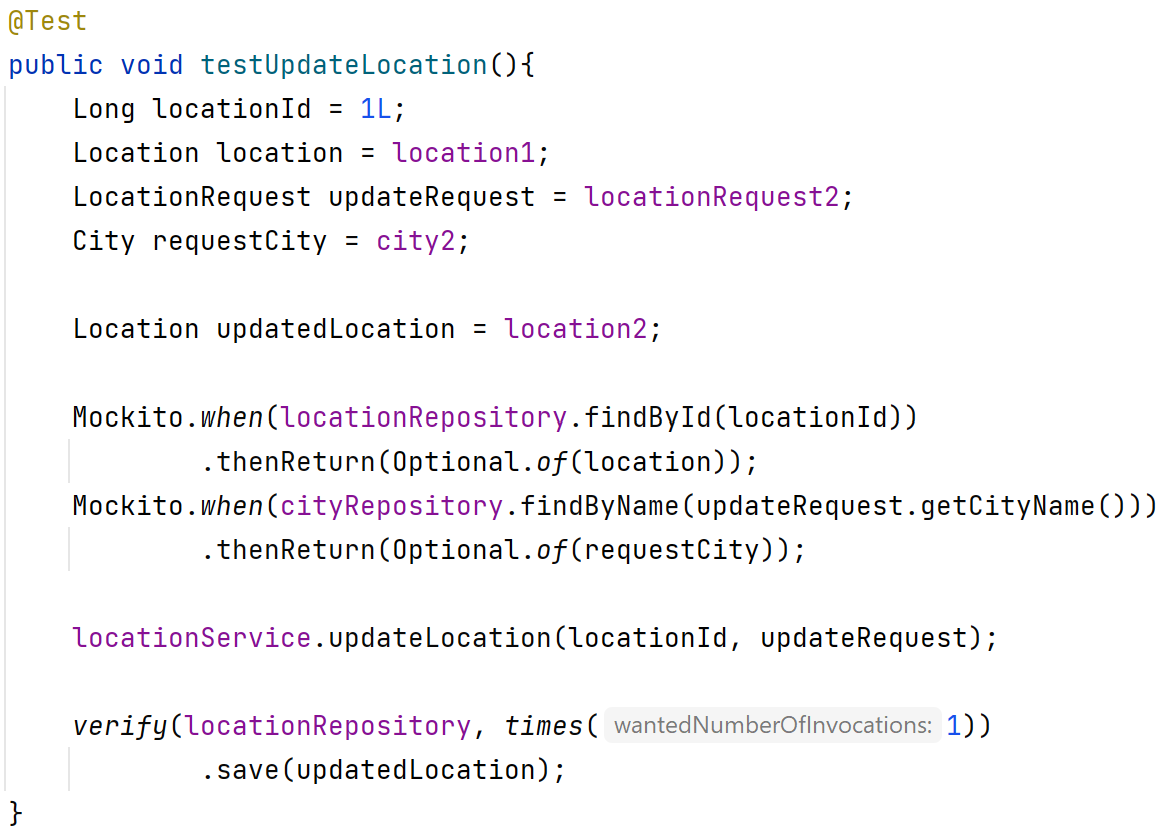
\includegraphics[scale=0.9]{slike/unit_test_location_update.png} 
              \centering
            \caption{Ispitni slučaj - razred \textit{BadgeService} - metoda \textit{updateLocation}}
        \end{figure}

        \begin{figure}[H]
            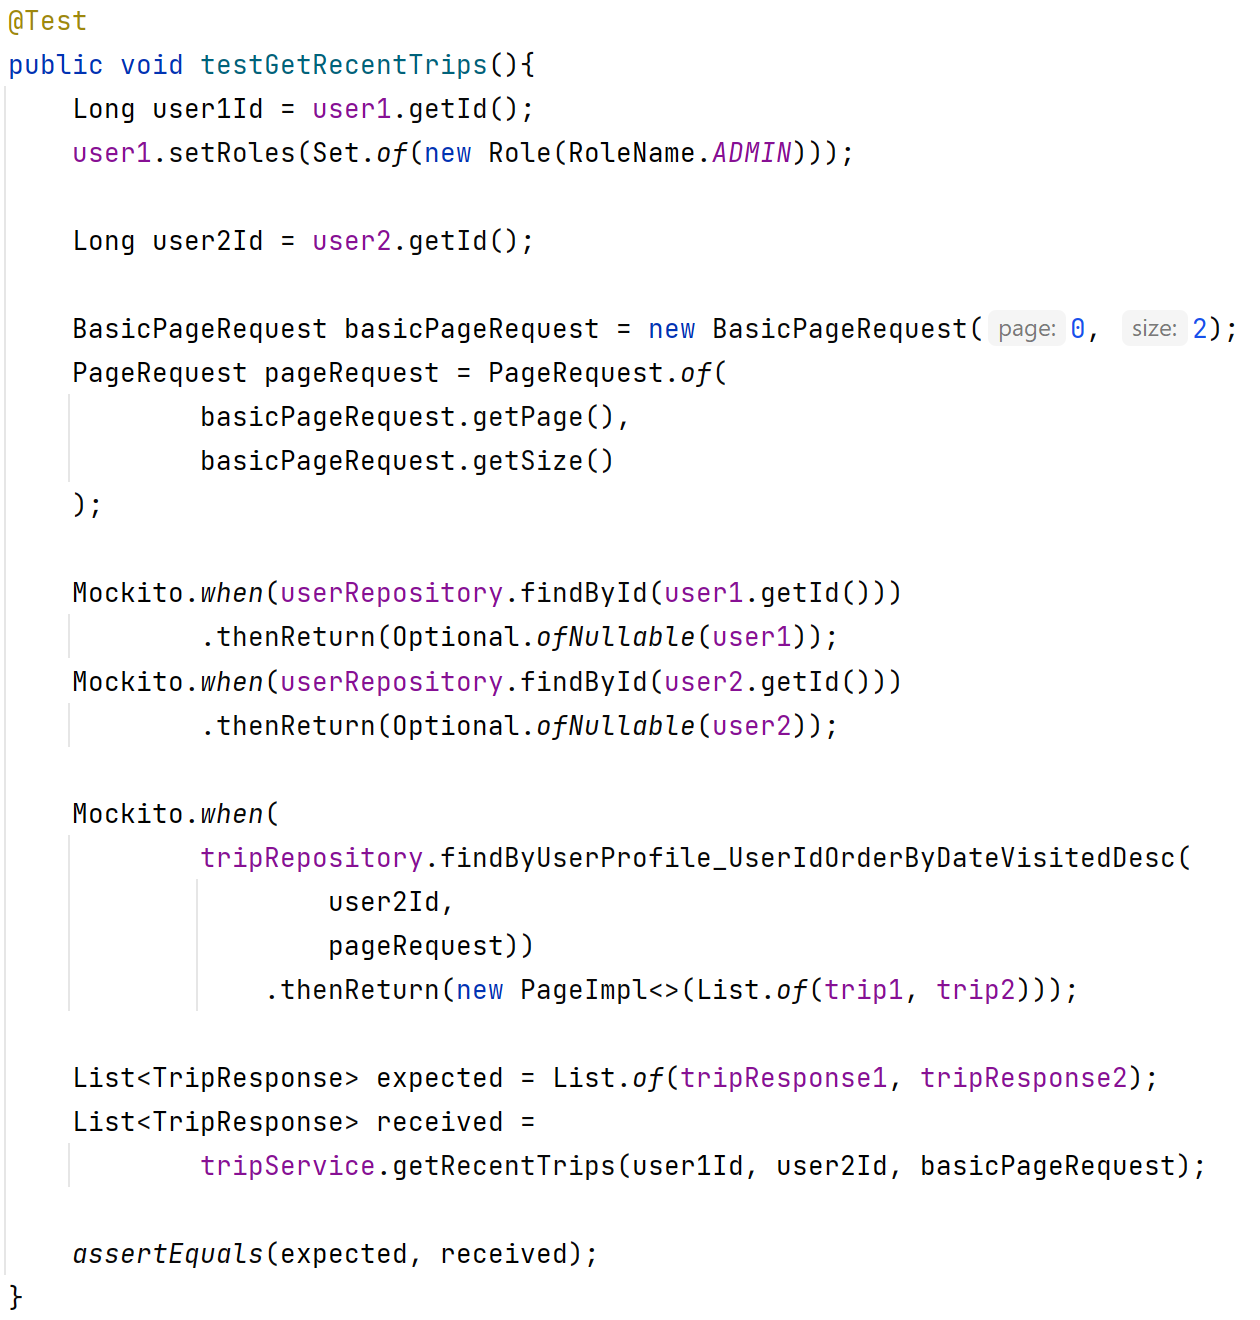
\includegraphics[scale=0.9]{slike/unit_test_trip_recent.png} 
              \centering
            \caption{Ispitni slučaj - razred \textit{TripService} - metoda \textit{getAllWonBadges} - bacanje iznimke}
        \end{figure}

        \begin{figure}[H]
            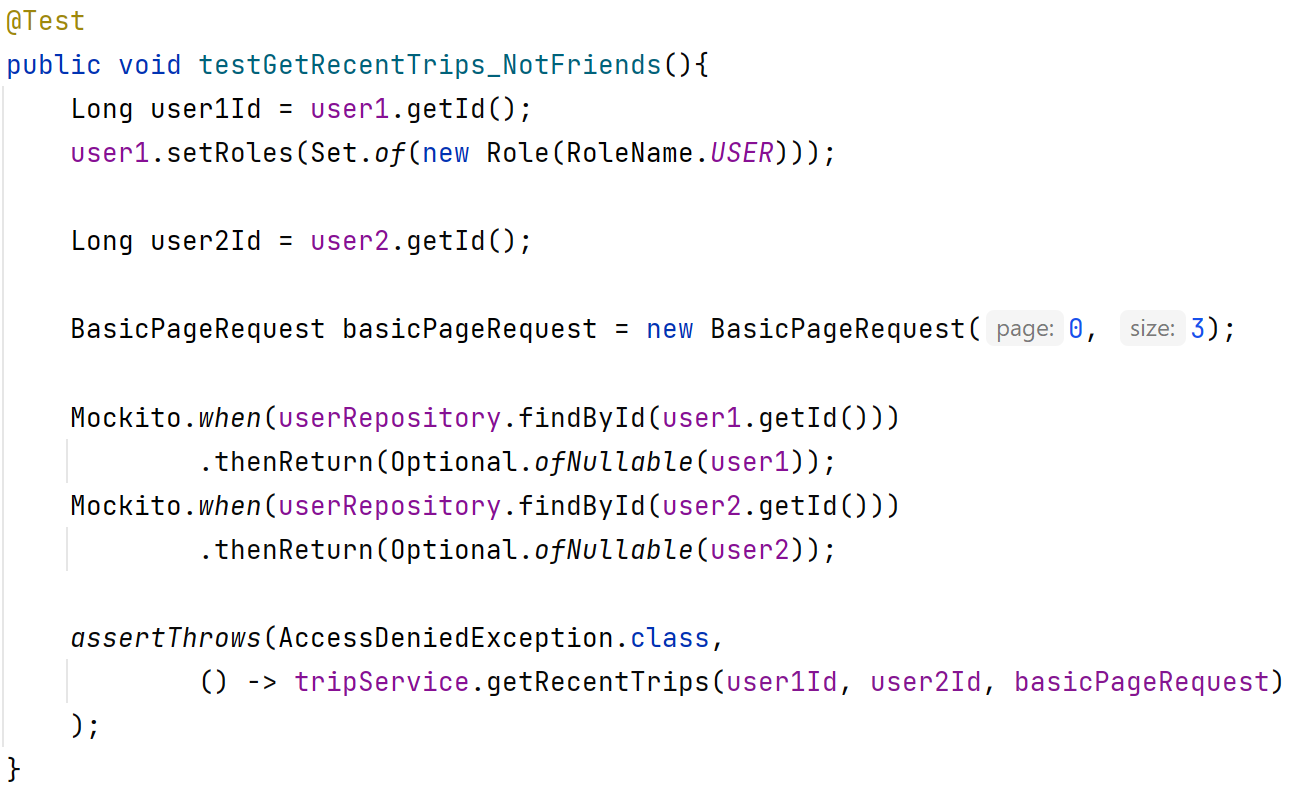
\includegraphics[scale=0.9]{slike/unit_test_trip_not_friends.png} 
              \centering
            \caption{Ispitni slučaj - razred \textit{TripService} - metoda \textit{getRecentTrips} - bacanje iznimke}
        \end{figure}

        \begin{figure}[H]
            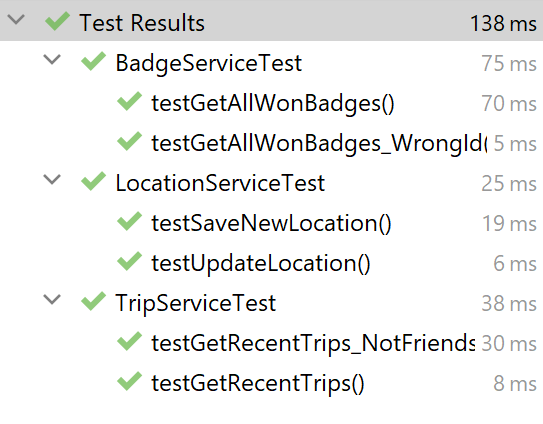
\includegraphics[scale=1]{slike/unit_test_results.png} 
              \centering
            \caption{Rezultati ispitivanja komponenti}
        \end{figure}
        \eject
        
			
			\subsection{Ispitivanje sustava}
			
			 Provedeno je ispitivanje sustava koristeći \underline{\href{https://www.selenium.dev/}{Selenium WebDriver}} (uz Chrome-ov WebDriver) u programskom jeziku Java uz pomoć okvira za jedinično ispitivanje \underline{\href{https://junit.org/junit5/}{JUnit}}. 
            \\
            \\
            Konstante koje završavaju na \textit{XPATH} predstavljaju izravnu putanju do elementa na stranici. Konstanta \textit{{BASE\_URL}} predstavlja URL web stranice. Prije pokretanja testova pokreće se funkcija \textit{initDriver()} koja inicijalizira WebDriver. 
            \\
            \\
            Kako bi se uspješno izvršili ispitni slučajevi u sustavu mora postojati registrirani korisnik s korisničkim imenom "\textit{user}" te lozinkom "\textit{password123}" te ne smije postojati korisnik s korisničkim imenom "\textit{NameSurname}".

                \begin{figure}[H]
        		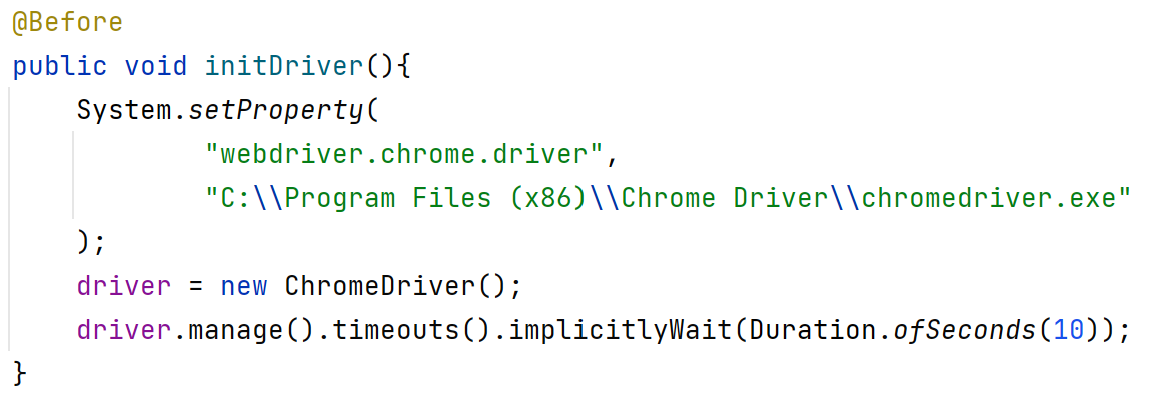
\includegraphics[scale=1]{slike/integration_test_init.png} 
        		  \centering
        		\caption{Inicijalizacija WebDriver-a}
        	\end{figure}

                \begin{figure}[H]
        		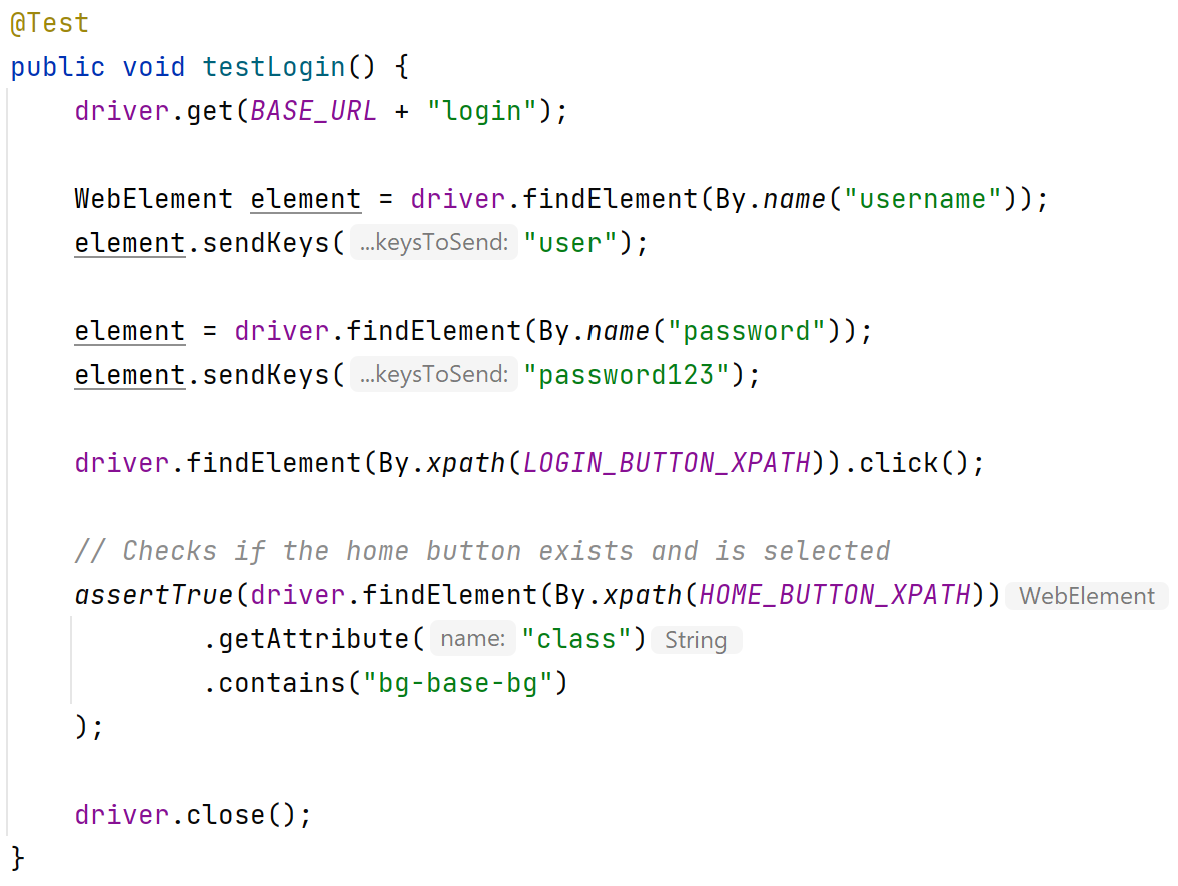
\includegraphics[scale=1]{slike/integration_test_login.png}
        		  \centering
        		\caption{Ispitni slučaj - prijava}
        	\end{figure}
                
                \begin{figure}[H]
        		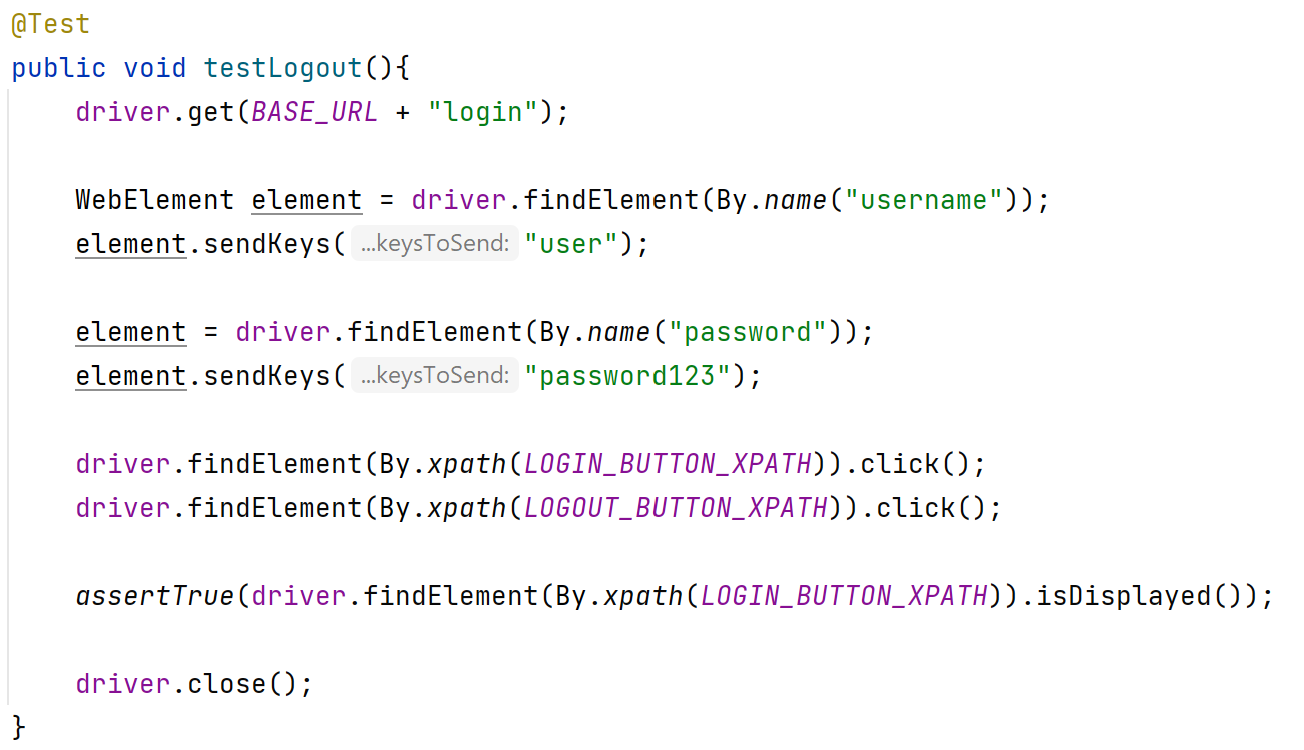
\includegraphics[scale=0.9]{slike/integration_test_logout.png} 
        		  \centering
        		\caption{Ispitni slučaj - odjava}
        	\end{figure}

                \begin{figure}[H]
        		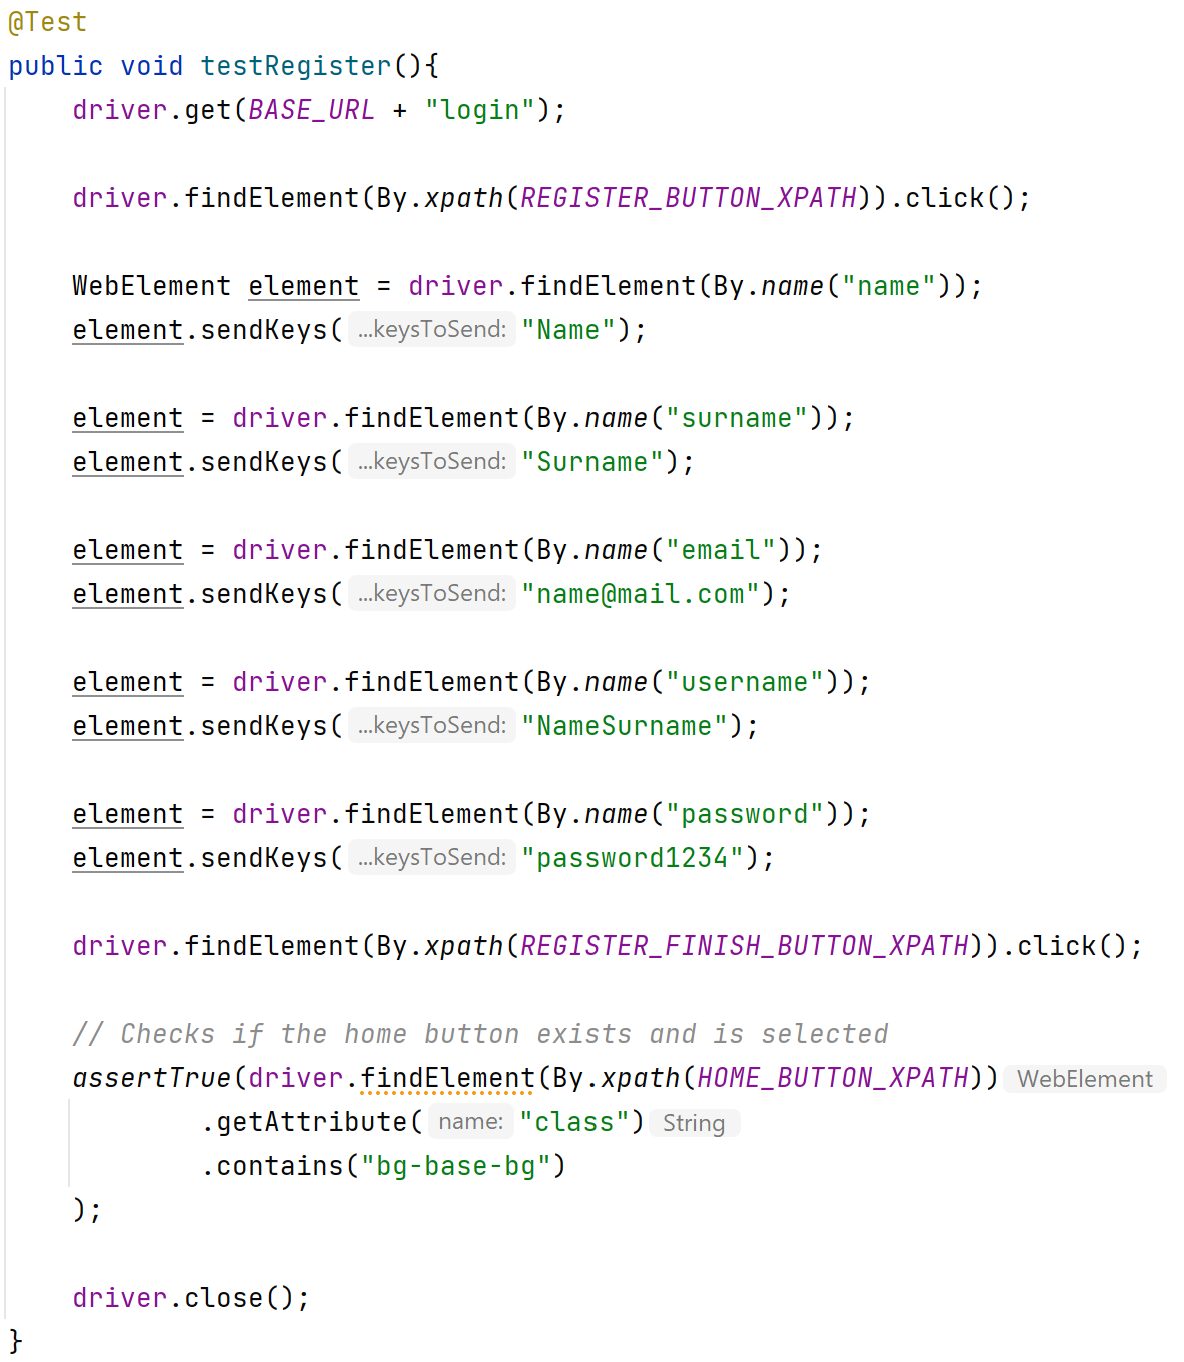
\includegraphics[scale=1]{slike/integration_test_register.png} 
        		  \centering
        		\caption{Ispitni slučaj - registracija}
        	\end{figure}

                \begin{figure}[H]
        		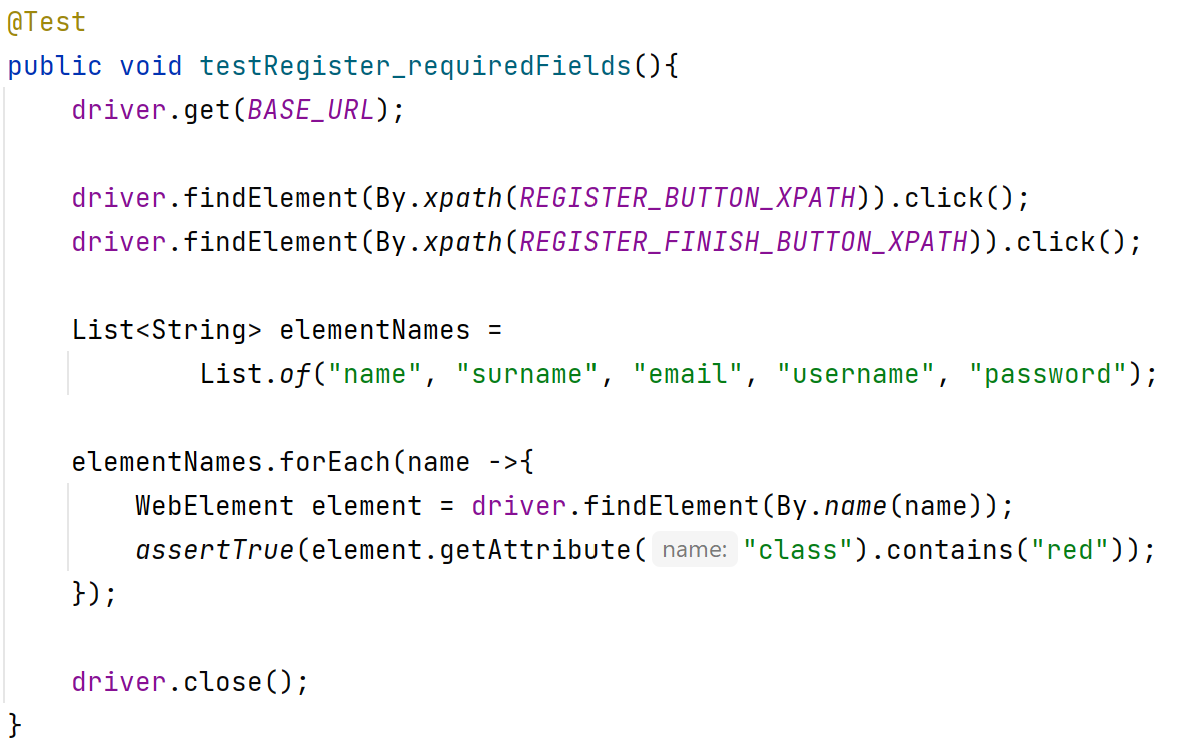
\includegraphics[scale=1]{slike/integration_test_register_required_fields.png} 
        		  \centering
        		\caption{Ispitni slučaj - validacija polja tijekom registracije}
        	\end{figure}
   
                \begin{figure}[H]
        		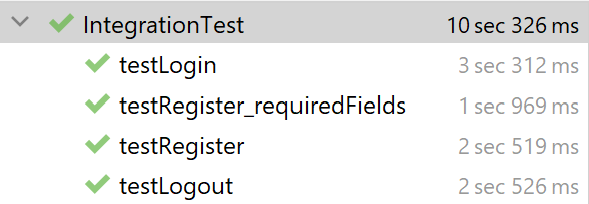
\includegraphics[scale=1]{slike/integration_test_results.png} 
        		  \centering
        		\caption{Rezultati ispitivanja sustava}
        	\end{figure}
		
			\eject 
		
		
		\section{Dijagram razmještaja}
			
			%\textbf{\textit{dio 2. revizije}}
			
			 %\textit{Potrebno je umetnuti \textbf{specifikacijski} dijagram razmještaja i opisati ga. Moguće je umjesto specifikacijskog dijagrama razmještaja umetnuti dijagram razmještaja instanci, pod uvjetom da taj dijagram bolje opisuje neki važniji dio sustava.}

            Dijagram razmještaja opisuje topologiju sklopovlja i programsku potporu koja se koristi u implementaciji. Korisnici koriste web preglednik kako bi pristupili web aplikaciji. Trenutna implementacija koristi dva različita poslužitelja, Heroku kao \textit{backend} poslužitelja i Render kao \textit{frontend} poslužitelja i poslužitelja baze podataka.
			\begin{figure}[H]
        		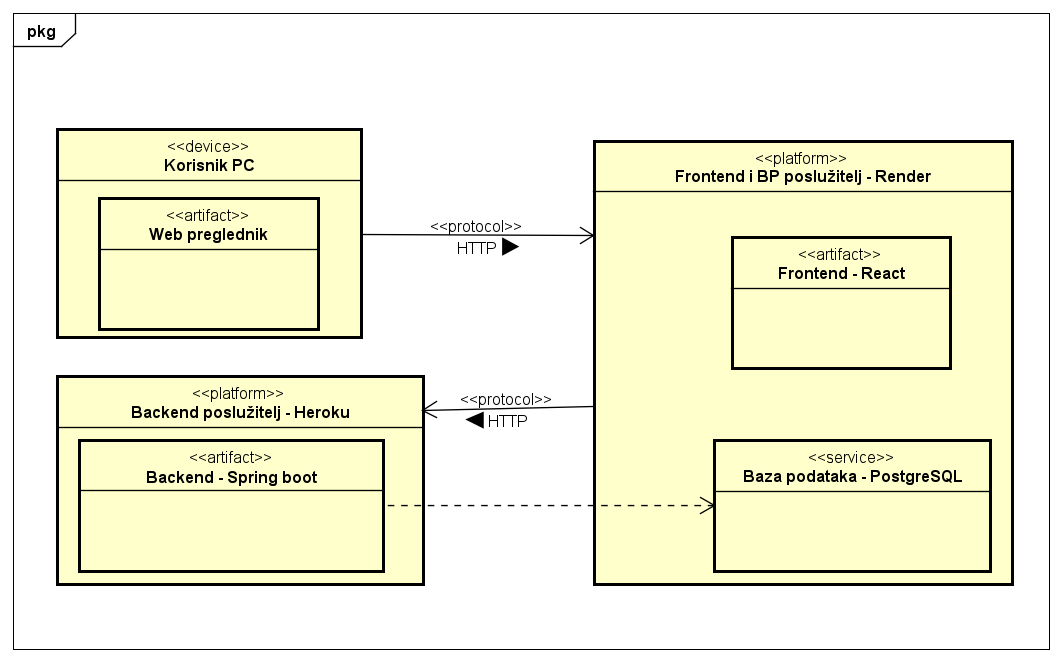
\includegraphics[scale=0.55]{slike/Dijagram razmjeÅ¡taja.png} %veličina slike u odnosu na originalnu datoteku i pozicija slike
        		  \centering
        		\caption{Dijagram razmještaja}

        	\end{figure}
			\eject 
		
		\section{Upute za puštanje u pogon}
		
			%&\textbf{\textit{dio 2. revizije}}\\
		
			% \textit{U ovom poglavlju potrebno je dati upute za puštanje u pogon (engl. deployment) ostvarene aplikacije. Na primjer, za web aplikacije, opisati postupak kojim se od izvornog kôda dolazi do potpuno postavljene baze podataka i poslužitelja koji odgovara na upite korisnika. Za mobilnu aplikaciju, postupak kojim se aplikacija izgradi, te postavi na neku od trgovina. Za stolnu (engl. desktop) aplikaciju, postupak kojim se aplikacija instalira na računalo. Ako mobilne i stolne aplikacije komuniciraju s poslužiteljem i/ili bazom podataka, opisati i postupak njihovog postavljanja. Pri izradi uputa preporučuje se \textbf{naglasiti korake instalacije uporabom natuknica} te koristiti što je više moguće \textbf{slike ekrana} (engl. screenshots) kako bi upute bile jasne i jednostavne za slijediti.}
			
			
			 %\textit{Dovršenu aplikaciju potrebno je pokrenuti na javno dostupnom poslužitelju. Studentima se preporučuje korištenje neke od sljedećih besplatnih usluga: \href{https://aws.amazon.com/}{Amazon AWS}, \href{https://azure.microsoft.com/en-us/}{Microsoft Azure} ili \href{https://www.heroku.com/}{Heroku}. Mobilne aplikacije trebaju biti objavljene na F-Droid, Google Play ili Amazon App trgovini.}

            \textbf{Instalacija poslužitelja baze podataka}
            \\
            Potrebno je preuzeti Docker Desktop aplikaciju. Za operacijski sustav Windows potrebno je instalirati i WSL2 podršku. Provodi se standardna instalacija s postavljanjem korisnika.
            \\
            \\
            \textbf{Pokretanje poslužitelja baze podataka}
            \\
    	Nakon instalacije potrebno je pokrenuti Docker kontejner preko `docker-compose.yaml` datoteke. Pozicionira se u direktorij gdje se datoteka nalazi te se pokreće korištenjem naredbe `docker-compose up`. U datoteci se nalazi potrebna konfiguracija za podizanje PostgreSQL baze podataka, sa postavljenim sučeljima i informacijama za spajanje.
            \\
            \\
            \textbf{Pokretanje poslužiteljske strane aplikacije}
            \\
            Potrebno je instalirati Gradle i Java programsku podršku. Nakon instalacije potrebno se pozicionirati u root direktorij aplikacije te pokrenuti naredbu `gradlew assemble`. Nakon što se aplikacija kompajlira, za pokretanje je potrebno upisati naredbu "`java -jar build/libs/[naziv\_izvršne\_datoteke].jar`.
            \\
            \\
            \textbf{Spajanje sa bazom podataka}
            \\
            Za stvaranje konekcije prema bazi podataka koristi se konfiguracija unutar aplikacije. Za aplikaciju je pri pokretanju potrebno definirati sve varijable okruženja potrebne za konfiguraciju, kao što su varijable za spajanje na bazu podataka. Primjer: `java -jar build/libs/app.jar -Dserver.port=8080 -DB\_URL=jdbc:postgresql://db.url -DB\_USERNAME=username -DB\_PASSWORD=password -DB\_SCHEMA=schema`.
            \\
            \eject
            \\
            \textbf{Pokretanje klijentske strane aplikacije}
            \\
            Za pokretanje klijentske strane potrebno je instalirati Node.js programsku podršku. Nakon instalacije potrebno se pozicionirati u root direktorij poslužiteljske aplikacije te izvršiti naredbu `npm run build`. Nakon izgradnje statičke stranice sa svim potrebnim resursima, poslužiteljska aplikacija za serviranje tih resursa pokreće se naredbom `npm start`.
            \\
            \\
            \textbf{Spajanje klijentske i poslužiteljske strane aplikacije}
            \\
            Isto kao i kod spajanja na bazu podataka, klijentska aplikacija ima konfiguriranog posrednika (eng. "proxy") pomoću kojeg se spaja prema poslužiteljskoj aplikaciji. Potrebno je dodati varijable okruženja pri pokretanju aplikacije. Primjer: `PORT=3000 APP\_BASE\_URL=https://url.do.posluzitelja node app.js
            
			
			\eject 

	\chapter{Zaključak i budući rad}
		
		%\textbf{\textit{dio 2. revizije}}\\
		
		%\textit{U ovom poglavlju potrebno je napisati osvrt na vrijeme izrade projektnog zadatka, koji su tehnički izazovi prepoznati, jesu li riješeni ili kako bi mogli biti riješeni, koja su znanja stečena pri izradi projekta, koja bi znanja bila posebno potrebna za brže i kvalitetnije ostvarenje projekta i koje bi bile perspektive za nastavak rada u projektnoj grupi.}
		
		 %\textit{Potrebno je točno popisati funkcionalnosti koje nisu implementirane u ostvarenoj aplikaciji.}

            Zadatak grupe "DJUNGELSKOG" je bio razvoj web aplikacije za praćenje putovanja po svijetu i dijeljenje istih sa prijateljima. Nakon 17 tjedana rada na aplikaciji ostvaren je cilj i aplikacija "Svjetski putnik" je u potpunosti izrađena.
            \\
            Izradu projekta možemo promatrati u dvije faze, svaka odgovara jednom ciklusu predavanja semestra. U prvoj fazi primaran cilj je bio upoznat se i osmisliti kako ostvariti aplikaciju te postići funkcionalnu alfa inačicu web aplikacije. 
            Česti sastanci tima su omogućili dobru organiziranost i koliko god moguću ravnomjernu raspodijelu posla unutar tima.
            \\
            Druga faza projekta je bila različita od prve, primarno je bilo jako puno intenzivnog rada kako bi se ispunili \textit{deadline}-ovi. Dio tima se prvi put susreo sa određenim tehnologijama te je bilo potrebno uložiti dosta vremena kako bi ih se naučilo koristiti. S obzirom na dobar plan iz prve faze projekta, u drugoj fazi je tim samo trebao pratiti navedeni plan što je u konačnici dovelo do gotovog proizvoda.
            \\
            Kroz obje faze su se izrađivali UML dijagrami koji opisuju funkcionalnost aplikacije iz različitih perspektiva. Osim dijagrama izrađena je dokumentacija koja opisuje velik dio funkcionalnosti projekta i služi budućim korisnicima kao pomoć pri uporabi aplikacije ili izmjenama aplikacije.
            \\
            Moguće proširenje postojeće inačice sustava je izrada mobilne aplikacije te dodavanje 3D modela posjećenih objekata bedževima kako bi se postigla zanimljivija estetika.
            \\
            Sudjelovanje na ovakvom projektu omogućilo je svim članovima tima stjecanje vrijednog iskustva rada u timu te upoznavanja novih tehnologija i dokumentiranja većeg projekta. Kao tim zadovoljni smo postignutim rješenjem i uspjehom jer smo uspjeli ostvariti cilj uz sve druge obaveze koje svaki član tima ima.
            \\
            
		
		\eject  
	\chapter*{Popis literature}
		\addcontentsline{toc}{chapter}{Popis literature}
	 	
 		\textbf{\textit{Kontinuirano osvježavanje}}
	
		
		
		\begin{enumerate}
			
			
			\item  Programsko inženjerstvo, FER ZEMRIS, \url{http://www.fer.hr/predmet/proinz}
			
			\item  I. Sommerville, "Software engineering", 8th ed, Addison Wesley, 2007.
			
			\item  The Unified Modeling Language, \url{https://www.uml-diagrams.org/}
			
			\item  Astah Community, \url{http://astah.net/editions/uml-new}
		\end{enumerate}
		
		 
	
	
	\begingroup
	\renewcommand*\listfigurename{Indeks slika i dijagrama}
	%\renewcommand*\listtablename{Indeks tablica}
	%\let\clearpage\relax
	\listoffigures
	%\vspace{10mm}
	%\listoftables
	\endgroup
	\addcontentsline{toc}{chapter}{Indeks slika i dijagrama}


	
	\eject 
		
	\chapter*{Dodatak: Prikaz aktivnosti grupe}
		\addcontentsline{toc}{chapter}{Dodatak: Prikaz aktivnosti grupe}

		\section*{Dnevnik sastajanja}

		\begin{packed_enum}
			\item  sastanak
			\item[] \begin{packed_item}
				\item Datum: 14. listopada 2022.
				\item Prisustvovali: Svi članovi
				\item Teme sastanka:
				\begin{packed_item}
					\item  upoznavanje članova
					\item  raspravljanje o podjeli posla
					\item  inicijalni "brainstorming"
				\end{packed_item}
			\end{packed_item}

			\item  sastanak
			\item[] \begin{packed_item}
				\item Datum: 23. listopada 2022.
				\item Prisustvovali: Svi članovi
				\item Teme sastanka:
				\begin{packed_item}
					\item  inicijalni oblik baze podataka
					\item  razrađivanje projektnog zadatka
				\end{packed_item}
			\end{packed_item}

			\item  sastanak
			\item[] \begin{packed_item}
				\item Datum: 30. listopada 2022.
				\item Prisustvovali: Svi članovi
				\item Teme sastanka:
				\begin{packed_item}
					\item  raspored posla do idućeg sastanka
					\item  dizajn ekrana aplikacije - funkcionalost i \textit{Frontend} dizajn
				\end{packed_item}
			\end{packed_item}

			\item  sastanak
			\item[] \begin{packed_item}
				\item Datum: 08. studenog 2022.
				\item Prisustvovali: Svi članovi
				\item Teme sastanka:
				\begin{packed_item}
					\item  raspored posla do "laboratorijske vježbe" demonstracije do sad napravljenog posla.
				\end{packed_item}
			\end{packed_item}

			\item  sastanak
			\item[] \begin{packed_item}
				\item Datum: 15. studenog 2022.
				\item Prisustvovali: Svi članovi
				\item Teme sastanka:
				\begin{packed_item}
					\item  pregled do sada napravljenog posla i preostalog posla
					\item raspodjela posla do predaje projekta za kraj 1. ciklusa nastave
				\end{packed_item}
			\end{packed_item}

                \item  sastanak
			\item[] \begin{packed_item}
				\item Datum: 10. prosinca 2022.
				\item Prisustvovali: Svi članovi
				\item Teme sastanka:
				\begin{packed_item}
					\item  pregled i raspodjela glavnog posla za 2. ciklus
					\item  druženje unutar tima pomoću aplikacije Discord
				\end{packed_item}
			\end{packed_item}

                \item  sastanak
			\item[] \begin{packed_item}
				\item Datum: 10. siječnja 2022.
				\item Prisustvovali: Svi članovi
				\item Teme sastanka:
				\begin{packed_item}
					\item  pregled napravljenog posla pred predaju
				\end{packed_item}
			\end{packed_item}

			%

		\end{packed_enum}

		\eject
		\section*{Tablica aktivnosti}


			\begin{longtblr}[
					label=none,
				]{
					vlines,hlines,
					width = \textwidth,
					colspec={X[7, l]X[1, c]X[1, c]X[1, c]X[1, c]X[1, c]X[1, c]X[1, c]},
					vline{1} = {1}{text=\clap{}},
					hline{1} = {1}{text=\clap{}},
					rowhead = 1,
				}
				\multicolumn{1}{c|}{} & \multicolumn{1}{c|}{\rotatebox{90}{\textbf{Ian Golob}}} & \multicolumn{1}{c|}{\rotatebox{90}{\textbf{Matej Košćec }}} &	\multicolumn{1}{c|}{\rotatebox{90}{\textbf{Edi Prodan }}} & \multicolumn{1}{c|}{\rotatebox{90}{\textbf{Zvonimir Žunić }}} &	\multicolumn{1}{c|}{\rotatebox{90}{\textbf{Josip Goluža }}} & \multicolumn{1}{c|}{\rotatebox{90}{\textbf{Adrian Sušec }}} &	\multicolumn{1}{c|}{\rotatebox{90}{\textbf{Ivan Kolar }}} \\
				Upravljanje projektom 		& 4 &  &  &  & &  & \\
				Opis projektnog zadatka 	&  &  &  &  &  & & 2 \\

				Funkcionalni zahtjevi       &  &  &  &  &  & & 2  \\
				Opis pojedinih obrazaca 	&  &  &  &  &  & & 6  \\
				Dijagram obrazaca 			&  &  &  &  &  & & 2  \\
				Sekvencijski dijagrami 		&  &  &  &  &  & & 6  \\
				Opis ostalih zahtjeva 		&  &  &  &  &  & & 1  \\

				Arhitektura i dizajn sustava	 &  &  &  &  & & & 5    \\
				Baza podataka				 & 10  &  &  &  & & & 4   \\
				Dijagram razreda 			 & 3  &  &  &  & & & 1   \\
				Dijagram stanja				&  &  &  &  &  & & 2&   \\
				Dijagram aktivnosti 		&  &  &  &  &  & & 2&  \\
				Dijagram komponenti			&  &  &  &  &  & & 2&  \\
				Korištene tehnologije i alati 		 & 1 & 0.5 & &  &  &  & 2 \\
				Ispitivanje programskog rješenja 	& 12 &  & & &  &  &  &  \\
				Dijagram razmještaja			&  &  &  & & &  & 1 &  \\
				Upute za puštanje u pogon 		&  & 1 &  & & &  &  &  \\
				Dnevnik sastajanja 			&  &  &  &  & & 2 &   \\
				Zaključak i budući rad 		&  &  &  &  & & & 2 &  \\
				Popis literature 			&  &  &  &  & & & 0.5 & \\
				&  &  &  &  &  &  &  \\ \hline
				Izrada baze podataka		 			 & 2 & 1 &  &  &  & \\
				Spajanje s bazom podataka 							& 0.5  &  &  &  &  &  &  \\
				Dizajn stranice 							& 5 & 15  &  10 & 3 &  & 8 & \\
				\textit{Backend} 							 & 58 & 65  & 20 & 9 & 26 & 35 & \\
				\textit{Frontend} 							 & 5 & 60  & 55 & 50 & 40 & 50 & \\
				Puštanje aplikacije u pogon     &  & 25  &  &  &  &  &  & \\
			\end{longtblr}


		\eject

		\section*{Dijagrami pregleda promjena}

		%\textbf{\textit{dio 2. revizije}}\\

		%\textit{Prenijeti dijagram pregleda promjena nad datotekama projekta. Potrebno je na kraju projekta generirane grafove s gitlaba prenijeti u ovo poglavlje dokumentacije. Dijagrami za vlastiti projekt se mogu preuzeti s gitlab.com stranice, u izborniku Repository, pritiskom na stavku Contributors.}
		                  \begin{figure}[H]
                			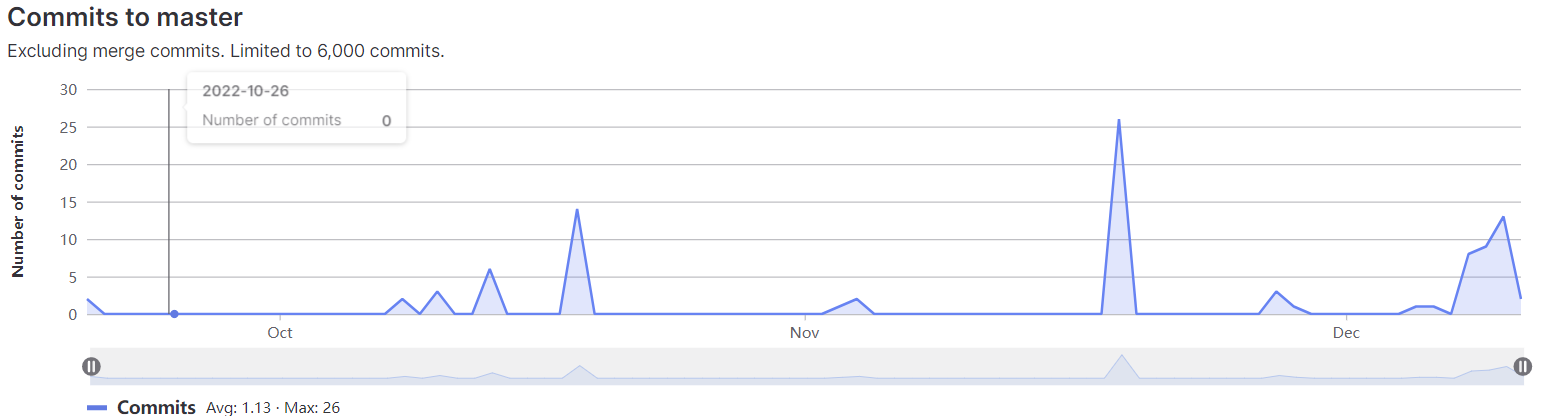
\includegraphics[scale=0.4]{slike/backend_master.PNG} %veličina slike u odnosu na originalnu datoteku i pozicija slike
                			\centering
                			\caption{Pregled promjena - \textit{backend}}
                			
                		\end{figure}

                            \begin{figure}[H]
                			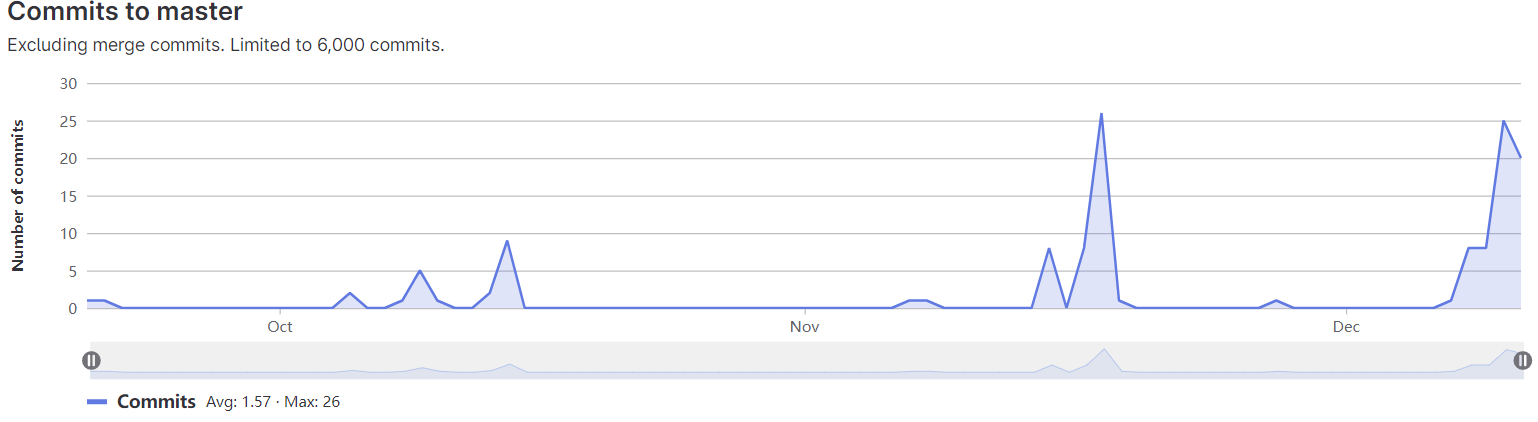
\includegraphics[scale=0.4]{slike/front_master.PNG} %veličina slike u odnosu na originalnu datoteku i pozicija slike
                			\centering
                			\caption{Pregled promjena - \textit{frontend}}
                			
                		\end{figure}
	


\end{document} %naredbe i tekst nakon ove naredbe ne ulaze u izgrađen dokument 


